% ------------------------------------------------------------------------
% Arquivo principal do TCC - Sandro Fadiga
% Template baseado no abnTeX2
% ------------------------------------------------------------------------
\documentclass[
    a4paper,
    12pt,                 % Tamanho da fonte
    oneside, 
    openright,
    english,              % Idioma adicional
    brazilian             % Idioma principal
]{abntex2}
% ------------------------------------------------------------------------
% Pacotes básicos
% ------------------------------------------------------------------------
\usepackage{lmodern}      % Usa a fonte Latin Modern
\usepackage[T1]{fontenc}  % Codificação da fonte
\usepackage[utf8]{inputenc} % Codificação do arquivo
\usepackage{lastpage}     % Contador de páginas
\usepackage{indentfirst}  % Indenta o primeiro parágrafo de cada seção
\usepackage{color}        % Controle das cores
\usepackage{graphicx}     % Inclusão de figuras
\usepackage{microtype}    % Melhora a justificação do texto
\usepackage{amsmath, amssymb, amsfonts}
\usepackage{float}        % Controle de posicionamento de figuras/tabelas
\usepackage{enumitem}     % Personalização de listas
\usepackage{booktabs}     % Tabelas mais profissionais
\usepackage{pdfpages}     % Inserir PDFs
\usepackage{caption}
\usepackage{subcaption}
\usepackage{longtable}    % Tabelas que quebram página
\usepackage{listings}     % Código fonte formatado
\usepackage{url}
\usepackage{hyperref}
\usepackage{epstopdf}
\usepackage{setspace}
\usepackage{textcomp}
\usepackage{array}
\usepackage{multirow}
% \usepackage{titlesec}     % Para controlar a formatação de títulos
\usepackage{listings}

% Pacotes para diagramas UML com TikZ
\usepackage{tikz}
\usepackage{pgf-umlcd}
\usetikzlibrary{positioning, shapes, arrows, calc, decorations.pathmorphing}

% Configurar lstlisting para português
\renewcommand\lstlistingname{Listagem}
\renewcommand\lstlistlistingname{Lista de Listagens}

% ------------------------------------------------------------------------
% CORREÇÃO: Força todos os títulos usarem a mesma fonte do texto
% ------------------------------------------------------------------------
\renewcommand{\ABNTEXchapterfont}{\rmfamily} % Remove itálico e negrito excessivo
\renewcommand{\ABNTEXchapterfontsize}{\normalsize\bfseries} % Tamanho normal com negrito

% ------------------------------------------------------------------------
% Configuração de hiperlinks
% ------------------------------------------------------------------------
\hypersetup{
    pdftitle={TCC - Sandro Fadiga},
    pdfauthor={Sandro Fadiga},
    pdfsubject={Protocolo de Peek/Poke para apoio à certificação de software embarcado},
    pdfcreator={LaTeX com abnTeX2},
    colorlinks=true,
    linkcolor=blue,
    citecolor=blue,
    urlcolor=blue
}
% ------------------------------------------------------------------------
% Informações de capa e folha de rosto
% ------------------------------------------------------------------------
\titulo{Depuração de Sistemas em Tempo Real:\\ Uma Abordagem de
Instrumentação de Código\\ para Testes de Sistemas Críticos.}
\autor{Sandro Fadiga}
\local{São Carlos}
\data{2025}
\instituicao{%
  Escola de Engenharia de São Carlos\\
  Universidade de São Paulo – USP}
\tipotrabalho{Trabalho de Conclusão de Curso (TCC)}

\preambulo{Monografia apresentada ao Curso de
Especialização em Sistemas Aeronáuticos da
Escola de Engenharia de São Carlos da
Universidade de São Paulo, como parte dos
requisitos para obtenção do título de
Especialista em Sistemas Aeronáuticos.
\\[0.5cm]
Orientador: Prof. Dr. Glauco Augusto de Paula Caurin
}

% ------------------------------------------------------------------------
% Início do documento
% ------------------------------------------------------------------------
\begin{document}

% Capa e folha de rosto
\imprimircapa
\imprimirfolhaderosto*

% ------------------------------------------------------------------------
% Elementos pré-textuais
% ------------------------------------------------------------------------
\newpage
% Texto de autorização no topo
{\small
\noindent
AUTORIZO A REPRODUÇÃO TOTAL OU PARCIAL DESTE TRABALHO, \\
POR QUALQUER MEIO CONVENCIONAL OU ELETRÔNICO, PARA FINS \\
DE ESTUDO E PESQUISA, DESDE QUE CITADA A FONTE.
}

\vspace{3cm}

% Linha da instituição
{\small
\noindent
Ficha catalográfica elaborada pela Biblioteca Prof. Dr. Sérgio Rodrigues Fontes da \\
EESC/USP com os dados inseridos pelo(a) autor(a).
}

\vspace{0.5cm}

% Caixa da ficha
\noindent
\begin{tabular}{|p{1.2cm}|p{13.5cm}|}
\hline
\multirow{16}{1.2cm}{F145d} & 
\textbf{Fadiga, Sandro Ferraz Martins} \\
& \quad Depuração de Sistemas em Tempo Real: Uma Abordagem de \\
& \quad Instrumentação de Código para Testes de Sistemas \\
& \quad Críticos.  / Sandro Ferraz Martins Fadiga; orientador \\
& \quad Glauco Augusto de Paula Caurin. São Carlos, 2025. \\
& \\
& \quad Especialização (Especialização em Sistemas \\
& \quad aeronáuticos) -- Escola de Engenharia de São Carlos da \\
& \quad Universidade de São Paulo, 2025. \\
& \\
& \quad 1. Sistemas embarcados. 2. Instrumentação de \\
& \quad código. 3. Injeção de valores. 4. Monitoramento de \\
& \quad variáveis. 5. Testes integrados. 6. Verificação de \\
& \quad software. 7. Software crítico. 8. Software tempo real. \\
& \quad I. Título. \\
\hline
\end{tabular}

\vspace{1cm}

% Rodapé
{\small
\noindent
Eduardo Graziosi Silva - CRB - 8/8907
}


\newpage

\begin{center}
    \textbf{\large FOLHA DE APROVAÇÃO}
\end{center}

\vspace{2.5cm}

\noindent



\newpage
\noindent
\textbf{DEDICATÓRIA}

\vspace{20cm}

\begin{flushright}
    \textit{Aos questionadores, aos inconformados, aos curiosos e aos \\ 
rebeldes, aqueles que movem o mundo para fora de suas \\
convicções e abrem novos caminhos para o conhecimento.}
\end{flushright}

\newpage
\begin{center}
    \textbf{\large AGRADECIMENTOS}
\end{center}

\vspace{1.5cm}

\noindent
Agradeço, primeiramente, à minha família, por me incentivar constantemente na 
busca pelo conhecimento e por acreditar nas minhas capacidades, mesmo nos 
momentos desafiadores.\\ 
Ao meu orientador, Prof. Dr. Glauco Augusto de Paula Caurin, pela dedicação, orientação precisa e valiosas contribuições que foram essenciais para o desenvolvimento deste trabalho. Aos demais professores do curso, pela transmissão de conhecimentos fundamentais e pelo suporte acadêmico fornecido ao longo desta jornada.\\
Aos colegas que tive a oportunidade de conhecer durante o curso, pelas trocas de conhecimentos, discussões enriquecedoras e pelo companheirismo que tornaram essa experiência ainda mais significativa.\\
Por fim, agradeço a todos que, de alguma forma, contribuíram para a realização deste trabalho.
\newpage

\vspace*{20cm}

\begin{flushright}
    \textit{``Program testing can show the presence of bugs} \\
    \textit{but not the absence.''} \\
    \vspace{0.5cm}
    (Edger W. Dijkstra, EWD303)
\end{flushright}

\newpage

\pagestyle{empty}

\chapter*{Resumo}

\noindent
FADIGA, S. F. M. \textbf{Depuração de Sistemas em Tempo Real}: Uma Abordagem de Instrumentação de Código para Testes de Sistemas Críticos. 2025. Monografia (Trabalho de Conclusão de Curso) – Escola de Engenharia de São Carlos, Universidade de São Paulo, São Carlos, 2025.

\vspace*{5mm}

\noindent
O desenvolvimento de sistemas embarcados de tempo real apresenta desafios específicos no que se refere à verificação e validação de requisitos, especialmente em ambientes de testes integrados, onde a capacidade de depuração é limitada. Ferramentas tradicionais de depuração, como probes e interfaces JTAG, não podem ser utilizadas durante a execução normal do software, exigindo abordagens alternativas. Este trabalho propõe o desenvolvimento de uma ferramenta de instrumentação de software embarcado, focada no monitoramento e injeção de valores em variáveis durante a execução dos sistemas. A solução será composta por três módulos principais: um protocolo simples de comunicação com o software embarcado, uma biblioteca em linguagem C para interpretação de comandos e acesso a variáveis internas, e uma interface gráfica no host para interação com o sistema embarcado. A ferramenta será projetada para testes integrados, como em ambientes Hardware-in-the-Loop (HIL), e visa auxiliar engenheiros na validação de sistemas críticos. Como produto final, será entregue uma prova de conceito (PoC) demonstrando o funcionamento da ferramenta, implementando operações de monitoramento (peek) e modificação (poke) de variáveis em tempo real.

\vspace*{5mm}

\noindent
\textbf{Palavras-chave:} Sistemas Embarcados, Instrumentação de Código, Injeção de valores, Monitoramento de Variáveis, Testes Integrados, Verificação de software, Software crítico, Software de tempo real.

\pagestyle{empty}

\chapter*{Abstract}

\noindent
FADIGA, S. F. M. \textbf{Debugging Real-Time Systems}: A Code Instrumentation Approach for
Testing Critical Systems. 2025. Monografia (Trabalho de Conclusão de Curso) –
Escola de Engenharia de São Carlos, Universidade de São Paulo, São Carlos, 2025.

\vspace*{5mm}

\noindent
The development of real-time embedded systems presents specific challenges regarding requirement verification and validation, especially in integrated testing environments where debugging capabilities are limited. Traditional debugging tools, such as probes and JTAG interfaces, cannot be used during normal software execution, requiring alternative approaches. This work proposes the development of an embedded code instrumentation tool, focused on monitoring and injecting values into variables during system execution. The solution comprises three main modules: a simple communication protocol with embedded code, a C language library for command interpretation and internal variable access, and a graphical host interface for interaction with the embedded system. The tool is designed for integrated testing, such as in Hardware-in-the-Loop (HIL) environments, and aims to assist engineers in validating critical systems. As a final product, a proof of concept (PoC) will be delivered demonstrating the tool's functionality, implementing real-time variable monitoring (Peek) and modification (Poke) operations.

\vspace*{5mm}

\noindent
\textbf{Keywords:} Embedded Systems, Code Instrumentation, Value Injection, Variable Monitoring, Integrated Testing, Software Verification, Critical Software, Real-Time Software.

\newpage
\lstlistoflistings
\newpage
\listoffigures*
\newpage
\listoftables*
\newpage
\tableofcontents*

% ------------------------------------------------------------------------
% Elementos textuais
% ------------------------------------------------------------------------
\textual
\chapter{Introdução}

\section{Contextualização}

A depuração de sistemas embarcados críticos de tempo real é de suma importância, pois assegura a segurança, a confiabilidade e a aderência aos requisitos de sistema. No que diz respeito aos requisitos de sistemas que devem ser desdobrados em requisitos de software para sistemas críticos, como os sistemas aeroespaciais aderentes à norma DO-178C, a depender do nível de criticidade do sistema em desenvolvimento é necessário comprovar a rastreabilidade do código associado aos requisitos de software para a devida geração de evidência de cobertura de requisitos.

O desafio, portanto, está associado a como, em testes de caixa preta, comprovar que requisitos estão sendo cumpridos. Para tais testes, usualmente estimula-se o sistema com entradas e coletam-se dados na saída. Este tipo de teste cobre requisitos de sistema no nível de integração de sistemas; porém, estes não são os únicos requisitos a serem verificados em um sistema crítico.

Muitos requisitos detalham estados ou cálculos intermediários de um sistema, de forma que sua aplicação nem sempre é passível de observação na saída do sistema. Existem ainda requisitos emergentes ou derivados, que surgem da necessidade de se criar uma solução no software para resolver um problema gerado pela solução de um requisito de sistema. Para tais requisitos, não é possível realizar medições nem, muitas vezes, estímulos de entrada em um teste de caixa preta.

Em sistemas de tempo real, cálculos e estados internos ao sistema estão associados à dimensão do tempo, usualmente sendo considerado o tempo de execução, ciclo ou de taxa como o tempo máximo permitido para a execução completa do ciclo do software, ou seja:

\begin{enumerate}
    \item Leitura e processamento de entradas;
    \item Cálculos com valores provenientes destas entradas (e valores provenientes de estados anteriores);
    \item Gravação em saída dos valores de cálculo.
\end{enumerate}

Neste modelo de execução, o software está submetido aos requisitos que definem margens de segurança, como o \textit{Worst-Case Execution Time} (WCET), o qual define quanto tempo o software pode ocupar no ciclo de execução total do sistema. Este tipo de requisito reserva um slot de tempo no sistema para o qual o software poderá ocupar na execução do seu ciclo. É necessária uma garantia de que o software em nenhum momento exceda o tempo total alocado, o qual vem acompanhado de uma margem de segurança.

Além da análise de WCET, são empregadas análises de cobertura estrutural do código, como o \textit{Modified Condition/Decision Coverage} (MCDC). Esse critério de cobertura é amplamente adotado em sistemas embarcados críticos, especialmente no contexto da certificação aeronáutica, conforme definido pela norma DO-178C \cite{rtca2011do178c}.

O critério MCDC é considerado um dos métodos mais rigorosos de cobertura estrutural, pois exige a verificação detalhada do impacto de cada condição lógica individual no resultado de uma decisão composta, contribuindo para a detecção de falhas que não seriam identificadas por critérios de cobertura menos restritivos \cite{Rierson2013}.

De forma mais específica, o MCDC impõe que os seguintes requisitos sejam atendidos:

\begin{enumerate}
    \item Cada condição atômica (subexpressão booleana dentro de uma decisão) seja avaliada como verdadeira e falsa ao menos uma vez;
    \item Cada decisão composta seja avaliada como verdadeira e falsa ao menos uma vez;
    \item Cada condição atômica demonstre influência independente sobre o resultado da decisão, exigindo a construção de casos de teste nos quais a alteração isolada de uma condição modifique o resultado final da decisão.
\end{enumerate}

Considerando, por exemplo, a decisão lógica apresentada no Código~\ref{lst:mcdc_exemplo}, composta pelas condições atômicas $A$, $B$ e $C$, a aplicação do critério MCDC requer a definição de casos de teste que demonstrem que cada uma dessas condições influencia de forma independente o resultado da decisão.

\begin{lstlisting}[language=C,
                   caption={Exemplo de decisão lógica para análise de MCDC},
                   label={lst:mcdc_exemplo}]
bool evaluate_decision(bool A, bool B, bool C) {
    if ((A && B) || C) {
        return true;
    } else {
        return false;
    }
}
\end{lstlisting}

Para se obter a cobertura completa de MCDC para as condições definidas no código apresentado na Listagem~\ref{lst:mcdc_exemplo}, é necessário, no mínimo, um conjunto de quatro casos de teste. Esse conjunto deve ser cuidadosamente projetado de forma a demonstrar, de maneira independente, a influência de cada condição atômica (A, B e C) no resultado da expressão booleana avaliada.

Em conformidade com o critério MCDC, cada condição deve assumir os valores verdadeiro e falso pelo menos uma vez, e deve ser possível evidenciar que a variação isolada de uma única condição é suficiente para alterar o resultado da decisão, mantendo-se as demais condições constantes.

\begin{enumerate}
    \item Condição A: Caso de teste quando apenas A difere, e a decisão total muda;
    \item Condição B: Caso de teste quando apenas B difere, e a decisão total muda;
    \item Condição C: Caso de teste quando apenas C difere, e a decisão total muda.
\end{enumerate}

A Tabela~\ref{tab:mcdc_casos_de_testes} apresenta o conjunto mínimo de casos de teste necessário para satisfazer esses critérios de cobertura.

\begin{table}[htbp]
    \centering
    \begin{tabular}{|c|c|c|c|c|}
        \hline
        \textbf{Teste} & \textbf{A} & \textbf{B} & \textbf{C} & \textbf{Resultado} \\
        \hline
        T1 & F & V & F & F \\
        \hline
        T2 & V & V & F & V \\
        \hline
        T3 & V & F & F & F \\
        \hline
        T4 & V & F & V & V \\
        \hline
    \end{tabular}
    \caption{Conjunto mínimo de casos de teste para cobertura MCDC}
    \label{tab:mcdc_casos_de_testes}
\end{table}

Portanto, como podemos verificar se requisitos de sistema, requisitos emergentes e de segurança estão sendo cumpridos pelo software, é necessária a verificação de valores e estados internos do software ao longo do tempo de execução. Assim, a questão central é: Como verificar tais valores sem interferir diretamente nos cálculos de valores e estados do sistema?

Ferramentas tradicionais de \textit{debug} são amplamente utilizadas na indústria de sistemas embarcados, sobretudo nos estágios iniciais do desenvolvimento do software sendo muito úteis para eliminar falhas e detectar erros iniciais de codificação dos requisitos. Ao se escolher a solução de hardware para o sistema, seleciona-se em conjunto, ou mesmo é fornecido pelo fabricante, um kit de desenvolvimento de software composto por:

\begin{itemize}
    \item Compilador para a linguagem de alto nível (normalmente C ou C++) para o hardware alvo;
    \item Algum mecanismo de comunicação entre o computador usado para o desenvolvimento do software e o hardware alvo;
    \item Um sistema de leitura e injeção de valores em memória do hardware;
    \item Alguma ferramenta de software para visualização e \textit{debug} de código, fazendo uso desta infraestrutura de comunicação e leitura/injeção de valores.
\end{itemize}

Contudo, as ferramentas de depuração fornecidas pelos fabricantes de microcontroladores, normalmente baseadas em interfaces como JTAG (Joint Test Action Group), SWD (Serial Wire Debug) ou hardware/sondas proprietárias são utilizadas em sua maioria durante as fases iniciais do desenvolvimento do software e seu uso é voltado para identificar e corrigir erros cometidos na codificação dos requisitos de baixo nível (ou nível de software), durante esta etapa testes formais ainda estão em etapa de desenvolvimento — tanto o software quanto os testes partem de um conjunto de requisitos em comum — que acontece em paralelo entre desenvolvimento e verificação.

Além disso, métodos convencionais de depuração — que pausam a execução ou utilizam single-stepping introduzem interferência no comportamento temporal do sistema, alterando sua dinâmica de execução e dificultando a verificação em tempo real que testes de requisitos e testes de integração com hardware na planta real necessitam manter.

Diante dessas limitações, torna-se evidente a necessidade de uma solução de depuração não intrusiva, padronizada e automatizável — capaz de operar sem dependência de sondas específicas nem de interfaces proprietárias, e que permita a execução de testes em ambientes representativos do sistema final.

\section{Motivação}

A depuração de sistemas embarcados críticos, especialmente aqueles de tempo real, enfrenta limitações quando se utilizam apenas técnicas tradicionais de testes de caixa preta. Muitos requisitos, incluindo requisitos derivados ou emergentes, só podem ser verificados por meio da observação de estados e valores internos do software durante sua execução. Ferramentas de depuração fornecidas pelos fabricantes, embora úteis, são geralmente complexas, custosas e voltadas ao desenvolvimento inicial, não sendo adequadas para fases de integração ou testes finais.

Nesse contexto, torna-se relevante desenvolver soluções específicas que permitam a inspeção controlada de estados internos do sistema sem comprometer sua execução. As operações de inspeção e modificação remota de memória — tradicionalmente conhecidas como \textit{peek} (leitura) e \textit{poke} (escrita) — constituem um dos mecanismos mais antigos e difundidos no contexto da depuração de sistemas computacionais e embarcados. Inicialmente popularizadas em plataformas de microcomputadores e linguagens interpretadas, essas operações foram posteriormente incorporadas ao desenvolvimento de sistemas embarcados como um meio simples e direto de acessar variáveis internas durante a execução \cite{dorfman2008obscurity}. Apesar das evoluções significativas em ferramentas e protocolos ao longo dos anos, o conceito permanece central para arquiteturas de depuração, sendo frequentemente encapsulado em interfaces padronizadas, APIs ou camadas de abstração \cite{singh2020peek}.

Embora a literatura acadêmica apresente limitações quanto à documentação formal de técnicas leves de depuração em plataformas de prototipagem, observa-se na prática que dispositivos amplamente utilizados, como Arduino e ESP32, incorporam utilitários de depuração em tempo real em seus ambientes de desenvolvimento. Tais mecanismos — muitas vezes implementados por meio de operações simples de leitura e escrita em memória (\textit{peek/poke}) ou via interfaces seriais — têm sido empregados por desenvolvedores para acelerar o processo de teste e validação durante o protótipo inicial de aplicações embarcadas. Apesar de não constituírem soluções completas de depuração nem substituírem métodos estruturados, essas ferramentas ilustram a demanda crescente por mecanismos acessíveis de inspeção e interação em tempo de execução, especialmente em projetos de propósito geral.

De maneira análoga, outras indústrias impõem normas específicas, como a ISO 26262 no setor automotivo, a IEC 62304 para dispositivos médicos e a IEC 61508 em sistemas de segurança funcional. Diante dessas exigências, fabricantes de microcontroladores e plataformas comerciais não disponibilizam, em geral, soluções de depuração do tipo peek/poke aptas a serem empregadas diretamente em sistemas críticos.

Ferramentas amplamente difundidas, como o Arduino Serial Monitor, o ESPIDF Monitor ou ambientes de desenvolvimento integrados (IDEs) fornecidos por fornecedores como STMicroelectronics (STM32CubeIDE) e Espressif, não contemplam processos de certificação de software e tampouco oferecem rastreabilidade de requisitos ou cobertura de testes exigida para níveis de criticidade elevados (DAL A e B, conforme o DO-178C).

Dessa forma, torna-se necessária a criação interna (in-house) de soluções de depuração adaptadas (tailored) ao sistema em desenvolvimento, de modo que o protocolo de comunicação, a arquitetura de software embarcado e as ferramentas de suporte sejam especificados, implementados e verificados em conformidade com o nível de garantia de desenvolvimento (Design Assurance Level – DAL) aplicável. Esse processo garante que cada requisito funcional seja rastreado, testado e documentado, permitindo que a ferramenta de depuração não comprometa a conformidade regulatória nem a integridade do sistema em operação.

\section{Objetivos}

\subsection{Objetivo Geral}

Propor, implementar e validar um protocolo simples de peek e poke para observação e modificação controlada de estados internos em sistemas embarcados de tempo real, a fim de apoiar atividades de teste e depuração.

\subsection{Objetivos Específicos}

\begin{itemize}
    \item Estudar os conceitos de depuração em sistemas embarcados e protocolos de comunicação aplicáveis;
    \item Definir os requisitos e a arquitetura de um protocolo de peek e poke;
    \item Implementar o protocolo em um microcontrolador de baixo custo (ex.: Arduino);
    \item Desenvolver uma ferramenta cliente para interação com o protocolo;
    \item Avaliar o funcionamento do protocolo em cenários de teste representativos.
\end{itemize}

\section{Justificativa}

A proposta deste trabalho se justifica pela necessidade de ferramentas acessíveis, específicas e de baixo custo para o teste e depuração de sistemas embarcados críticos. Diferentemente de soluções comerciais, que exigem infraestrutura complexa, o protocolo aqui desenvolvido visa oferecer uma alternativa prática tanto em contextos acadêmicos quanto em aplicações industriais. Assim, contribui para a formação de profissionais em sistemas embarcados, possibilita o aprofundamento em técnicas de teste e depuração, e ainda pode ser expandido em pesquisas futuras, incluindo integração com ambientes de simulação e ferramentas de verificação formal.

\section{Estrutura do Trabalho}

Este trabalho está organizado da seguinte forma:

\begin{itemize}
    \item \textbf{Capítulo 1 -- Introdução:} apresenta a contextualização do tema, a motivação, os objetivos, a justificativa e a organização do trabalho.
    
    \item \textbf{Capítulo 2 -- Fundamentação Teórica:} descreve os conceitos de sistemas embarcados de tempo real, técnicas de depuração e protocolos de comunicação, além de trabalhos relacionados.
    
    \item \textbf{Capítulo 3 -- Desenvolvimento do Protocolo:} detalha a arquitetura, a especificação e a implementação do protocolo proposto, tanto no microcontrolador quanto na ferramenta cliente.
    
    \item \textbf{Capítulo 4 -- Metodologia e Testes:} apresenta o ambiente de experimentação, a metodologia de avaliação e os resultados obtidos.
    
    \item \textbf{Capítulo 5 -- Conclusão e Trabalhos Futuros:} reúne as conclusões do trabalho, suas limitações e as perspectivas de continuidade.
\end{itemize}
      % Capítulo 1
\chapter{Fundamentação}


\section{Software Embarcado e Sistemas Críticos}

Segundo \cite{ieee2000}, software embarcado é aquele projetado para operar em um sistema computacional integrado a um sistema maior, geralmente sujeito a restrições de tempo real, memória e energia, além de interagir diretamente com o ambiente físico por meio de sensores e atuadores.

De forma mais simples, pode-se afirmar que o software embarcado é desenvolvido de maneira conjunta ao hardware no qual será executado. Em contraste com softwares voltados a computadores pessoais — nos quais a portabilidade entre plataformas similares é frequentemente possível, mesmo diante de diferenças de hardware — os sistemas embarcados são projetados para solucionar problemas de engenharia específicos. Consequentemente, o software precisa ser concebido de modo a satisfazer requisitos funcionais, temporais e estruturais definidos pela aplicação final, refletindo a forte dependência entre software e hardware.

\subsection{Características: tempo real, restrições de hardware e determinismo}

Um software embarcado apresenta diversas características fundamentais, entre elas comportamento de \textit{tempo real} e \textit{determinismo}. É comum associar “tempo real” ao tempo cronológico natural (tempo de relógio). Entretanto, em sistemas embarcados, tempo real refere-se à capacidade do software de executar suas funções dentro de limites temporais estritamente definidos durante a fase de projeto. Ou seja, o sistema deve garantir que o tempo necessário para a execução de cada ciclo não ultrapasse o tempo máximo alocado para aquelas operações.

Cada sistema embarcado possui janelas temporais definidas com base em cálculos de desempenho, processamento de entradas e saídas e margens de segurança necessárias para garantir operação confiável.

Uma consequência direta desse aspecto é o conceito de \textit{criticidade}, frequentemente associado a sistemas embarcados de tempo real. A criticidade, contudo, está mais relacionada ao sistema final e ao impacto de seu funcionamento sobre pessoas, bens ou o ambiente, do que ao software isoladamente — visto que o software, enquanto abstração, não é inerentemente perigoso.

\subsection{Software Crítico de Segurança}

Segundo \cite{Rierson2013}, software crítico de segurança (\textit{safety-critical software}) pode ser definido a partir do conceito mais amplo de segurança. Uma definição geral para segurança é a ``ausência de condições que possam causar morte, lesão, enfermidade, dano ou perda de equipamentos ou propriedade, ou prejuízo ao meio ambiente'' \cite{Rierson2013}. Já a definição específica de software crítico de segurança é mais subjetiva.

O Institute of Electrical and Electronic Engineers (IEEE) define software crítico de segurança como:
\begin{quote}
    ``Software cujo uso em um sistema pode resultar em risco inaceitável. Software crítico de segurança inclui software cuja operação, ou falha em operar, pode levar a um estado perigoso, software destinado a recuperar-se de estados perigosos e software destinado a mitigar a severidade de um acidente'' \cite{Rierson2013}.
\end{quote}

O \textit{NASA Software Safety Standard} identifica um software como crítico de segurança quando ao menos um dos seguintes critérios é satisfeito \cite{Rierson2013}:

\begin{itemize}
    \item O software causa ou contribui para uma condição de sistema que, caso não seja controlada, possa resultar em morte, lesão grave ou danos significativos ao equipamento, à propriedade ou ao meio ambiente.
    \item O software é responsável por detectar, monitorar ou controlar estados perigosos, condições anômalas ou situações que envolvam risco para pessoas, equipamentos ou missões.
    \item O software executa funções necessárias para mitigar, isolar ou responder a falhas do sistema ou do hardware, prevenindo que tais falhas se tornem condições inseguras.
    \item O software fornece informações críticas utilizadas para tomada de decisão operacional, segurança de voo, controle de missão ou manobras que, se incorretas, podem provocar um resultado perigoso.
    \item O software é utilizado em sistemas de apoio à missão, simulação, teste ou validação, cujo comportamento incorreto possa induzir erros em sistemas críticos de voo, operação ou segurança.
\end{itemize}

Portanto quando abordado neste texto os termos mais abrangentes como software embarcado ou software de tempo real estarão referindo-se ao termo mais específico e de interesse deste trabalho: software crítico de segurança.

\subsection{Aplicações de Software Embarcado em Setores de Alta Criticidade}

A crescente complexidade dos produtos tecnológicos, associada à pressão por ciclos de desenvolvimento mais curtos e maior capacidade de atualização, tem impulsionado o uso intensivo de software embarcado em diferentes segmentos industriais. O software, por ser mais flexível, reconfigurável e economicamente vantajoso do que soluções puramente baseadas em hardware, tornou-se elemento central no projeto de sistemas modernos. 

Embora diversos setores utilizem software embarcado, três deles se destacam pela elevada dependência de funções automatizadas e pelo impacto direto sobre a segurança humana: o setor aeroespacial, o automotivo e o médico-hospitalar. Esses domínios compartilham um aspecto fundamental: a necessidade de garantir níveis rigorosos de confiabilidade e segurança, o que exige a adoção de normas específicas para desenvolvimento, verificação, validação e certificação de software crítico.

\subsubsection{Setor Aeroespacial}

No setor aeroespacial, especialmente na aviação comercial, o software embarcado está presente em uma ampla gama de sistemas, desde módulos de entretenimento de cabine até sistemas de controle de voo, navegação, freios e gerenciamento de potência. A criticidade de cada função determina o rigor necessário no processo de desenvolvimento, sendo esses níveis formalizados pelo \textit{Design Assurance Level} (DAL), conforme estabelecido pela norma DO-178C.

Os níveis de criticidade variam de DAL~A a DAL~E, onde:
\begin{itemize}
    \item \textbf{DAL A} - \textbf{Catastrófico}: condições de falha que podem resultar em catástrofe.
    \item \textbf{DAL B} - \textbf{Severa}: condições de falha que podem resultar em falha severa do sistema, porém não catastrófica.
    \item \textbf{DAL C} - \textbf{Maior}: condições de falha que podem resultar em degradação importante do desempenho.
    \item \textbf{DAL D} - \textbf{Menor}: falhas que têm efeitos menores sobre a operação, inconveniencias.
    \item \textbf{DAL E} - \textbf{Sem Efeito}: falhas sem impacto na segurança operacional.
\end{itemize}

Sistemas classificados nos níveis A e B exigem evidências extensivas de verificação, rastreabilidade e cobertura estrutural, refletindo a criticidade de suas funções. Eventos recentes na indústria reforçam a importância de processos rigorosos de certificação e verificação de software em sistemas de controle de voo.

\subsubsection{Setor Automotivo}

No setor automotivo, a incorporação de sistemas embarcados evoluiu drasticamente nas últimas décadas, abrangendo desde sistemas de infoentretenimento até algoritmos de controle de estabilidade, freios ABS, \textit{airbags}, direção assistida e funções autônomas. Da mesma forma que na aviação, a segurança dos ocupantes e ambiente em torno ao veículo é o fator determinante para o rigor do processo de desenvolvimento. 

A norma de referência nesse domínio é a ISO~26262, que define os níveis de criticidade do \textit{Automotive Safety Integrity Level} (ASIL), que vão de ASIL~A (menor severidade) até ASIL~D (maior severidade). Os requisitos incluem análise de riscos, definição de métricas de segurança, validação e rastreabilidade de requisitos, e estratégias de teste orientadas a segurança funcional. Casos amplamente documentados na literatura técnica demonstram como falhas de software podem impactar diretamente a segurança veicular, reforçando a importância da conformidade com padrões rigorosos.

\subsubsection{Setor Médico-Hospitalar}

Na indústria médica, dispositivos embarcados tornaram-se essenciais para monitoramento, diagnóstico e tratamento. Equipamentos como bombas de infusão, respiradores, sistemas de radioterapia e equipamentos de imagem utilizam software que deve operar com precisão, confiabilidade e tolerância a falhas. 

As normas IEC~62304 e ISO~14971 regulamentam o ciclo de vida do software e a análise de riscos para dispositivos médicos, estabelecendo requisitos de engenharia, verificação e manutenção. Eventos históricos envolvendo falhas de software em máquinas terapêuticas de alta energia ilustram a gravidade potencial de erros em sistemas deste setor e motivaram o desenvolvimento das normas atualmente vigentes.

\subsubsection{Desafios Comuns: Testes e Certificação}

Apesar das diferenças entre os setores, um desafio comum permeia o desenvolvimento de software crítico de segurança: a necessidade de gerar evidências objetivas de segurança por meio de testes e campanhas de ensaios. Testes não apenas demonstram o atendimento aos requisitos definidos em projeto, mas também fornecem a documentação necessária a autoridades certificadoras para comprovar conformidade com normas de segurança. Em ambientes de alta criticidade, a ausência de testes rigorosos compromete não apenas o produto final, mas a viabilidade de sua certificação e entrada em operação.

\subsection{Importância da Previsibilidade Temporal}

A previsibilidade temporal é um dos pilares fundamentais no desenvolvimento de sistemas embarcados de tempo real, especialmente quando esses sistemas operam em contextos críticos à segurança. Em tais aplicações, não basta que o software produza resultados corretos: é igualmente essencial que esses resultados sejam entregues dentro de limites temporais previamente especificados. Assim, além de requisitos funcionais, sistemas de tempo real possuem requisitos temporais que devem ser rigorosamente atendidos \cite{Laplante2011}.

Em sistemas embarcados determinísticos, cada tarefa deve executar dentro de uma janela de tempo definida durante o projeto, frequentemente denominada \textit{tempo de ciclo} ou \textit{deadline}. O não cumprimento dessas restrições pode resultar em instabilidade, perda de controle, violação de margens de segurança ou até falhas catastróficas, dependendo do contexto operacional. Por essa razão, a análise do \textit{Worst-Case Execution Time} (WCET) é central nesses sistemas, pois fornece limites superiores para a duração de cada tarefa, garantindo que o sistema como um todo permaneça dentro de sua operação segura \cite{wilhelm2008wcet}.

Do ponto de vista da certificação, normas como DO-178C para sistemas aeronáuticos, ISO 26262 para sistemas automotivos e IEC 62304 para dispositivos médicos enfatizam a necessidade de demonstrar que o comportamento temporal do software é previsível e analisável. Embora tais normas não utilizem explicitamente o termo ``previsibilidade temporal'', elas exigem evidências de determinismo, ausência de comportamentos assíncronos não analisados, controle sobre latências internas e conformidade com requisitos temporais definidos. Esses requisitos mostram que a previsibilidade temporal é, de fato, um elemento estruturante do processo de verificação e validação em sistemas críticos.

Garantir previsibilidade temporal implica o monitoramento de métricas como latência, jitter, tempo de resposta e ocupação do ciclo de execução. Variações inesperadas nesses parâmetros podem indicar problemas de implementação, interferências entre tarefas, condições de corrida, priorização inadequada ou fluxo de execução ineficiente. Dessa forma, ferramentas capazes de observar, registrar e analisar esses fenômenos tornam-se essenciais durante o processo de teste e integração.

Nesse contexto, a ferramenta desenvolvida neste trabalho apoia diretamente a análise de previsibilidade temporal, permitindo a inspeção em tempo real de variáveis internas, estados intermediários e comportamento do ciclo de execução. Ao oferecer visibilidade sobre características temporais do software — sem interferir significativamente em sua operação — a ferramenta contribui para a identificação precoce de problemas, para a avaliação de requisitos temporais e para a produção de evidências de conformidade exigidas em processos de certificação.


\section{Testes em Sistemas Embarcados}

Podem-se dividir os testes de software em sistemas embarcados em dois grandes grupos: testes de requisitos de alto nível e testes de requisitos de baixo nível. A execução adequada desses dois grupos é essencial para comprovar a aderência a normas de certificação, como a DO-178C. Embora os testes representem apenas uma parte do esforço total de verificação exigido para a certificação de software crítico, eles constituem uma etapa central e complexa — sobretudo os testes de requisitos de alto nível, os quais derivam dos requisitos de sistema e devem demonstrar a capacidade do software de se integrar corretamente ao sistema do qual fará parte.

O objetivo dos testes de software é identificar erros introduzidos durante a implementação dos requisitos na linguagem de programação de alto nível, incluindo erros lógicos, de uso da linguagem e funcionais. Quanto maior o rigor na definição dos casos de teste, maior será a cobertura obtida e, consequentemente, maior a probabilidade de detectar falhas durante o desenvolvimento.

Os testes são organizados em três fases principais:

\begin{itemize}
\item \textbf{Testes de Desenvolvimento} — Nesta fase, o programador traduz os requisitos de alto e baixo nível para a linguagem de programação adotada. Os testes são executados em plataformas de desenvolvimento, que geralmente possuem baixa representatividade em relação ao sistema final.
\item \textbf{Testes de Requisitos de Software} — Nesta etapa, os testes são elaborados com base nos requisitos utilizados na codificação. Para cada requisito são definidos casos de teste específicos, podendo haver mais de um caso por requisito.
\item \textbf{Testes de Integração} — Os testes de integração são realizados em ambientes representativos do sistema final, abrangendo principalmente os requisitos de alto nível e os requisitos de sistema. Nessa fase, não é permitido o uso de instrumentos ou técnicas que possibilitem a coleta de informações internas do software de forma intrusiva, de modo a não interferir na execução normal do sistema.
\end{itemize}

O presente trabalho tem como objetivo auxiliar as etapas de testes de requisitos e, especialmente, de testes de integração, nas quais o uso de kits de desenvolvimento deixa de ser adequado e o ambiente de testes deve apresentar maior representatividade em relação ao sistema final. Em sistemas aeroespaciais, é comum que a fase final de testes ocorra em um ambiente denominado Iron Bird, que consiste em um laboratório contendo todos os sistemas reais da aeronave conectados e configurados para ensaios de integração. Nesse ambiente, não é possível empregar técnicas de depuração que interrompam a execução do software para inspeção de seu estado interno. Assim, ferramentas de peek/poke tornam-se particularmente valiosas.

\section{Protocolos de Comunicação para Depuração}

A comunicação entre ferramentas de depuração e sistemas embarcados desempenha um papel essencial no processo de verificação e validação, sobretudo em ambientes nos quais o acesso físico aos sinais internos do software é limitado ou inexistente. Para que seja possível realizar operações de inspeção, monitoração ou injeção de valores — como nos mecanismos de peek/poke — é necessário o uso de protocolos de comunicação confiáveis, determinísticos e adequados às restrições do sistema embarcado.

Diversos meios físicos e protocolos são tradicionalmente empregados para esse fim, entre os quais se destacam UART, CAN e Ethernet. Cada um desses protocolos apresenta vantagens e limitações específicas, e normalmente sua escolha também está associada a escolha da arquitetura do sistema no qual o software irá executar, sendo assim uma decisão sistemica e mais abrangente, é comum o protocolo estar associado a uma restrição física imposta por decisões no nível de hardware, sejam elas derivadas de requisitos de custo ou requisitos funcionais ou até mesmo comerciais por imposições advindas da escolha de fornecedores. A caracteristica comum a todas os protocolos escolhidos é que sigam o paradigma de comunicação serial. 

\begin{itemize}
\item \textbf{UART} — A comunicação via UART é simples, de baixo custo e amplamente disponível, porém oferece taxas de transmissão relativamente limitadas e menor robustez contra erros. 
\item \textbf{CAN} — O barramento CAN fornece elevada imunidade a ruído e mecanismos nativos de priorização de mensagens, sendo bastante apropriado para ambientes automotivos e aeroespaciais, mas possui capacidade de carga útil reduzida por quadro. 
\item \textbf{Ethernet} — O protocolo Ethernet apresenta alta velocidade e baixa latência, porém exige uma camada extra que garanta seu uso em sistemas embarcados de tempo real/críticos o que pode introduzir sobrecarga e maior custo de implementação em sistemas embarcados críticos.
\end{itemize}

Independentemente do meio físico adotado, protocolos de depuração geralmente seguem um modelo de comunicação request/response, no qual uma ferramenta externa envia comandos e o dispositivo embarcado responde de forma determinística. Esse paradigma facilita a rastreabilidade das interações e permite que comandos sejam estruturados de forma padronizada, com semântica clara e verificável. Para garantir a correta interpretação das mensagens, é fundamental definir mecanismos de framing, incluindo marcação de início e fim de pacote, numeração de sequência e regras explícitas de encapsulamento dos dados.

A confiabilidade da comunicação depende também da detecção de erros. Por esse motivo, técnicas de checagem de integridade, como checksums ou Cyclic Redundancy Checks (CRC), são amplamente utilizadas. O CRC destaca-se pela capacidade de detectar padrões de erro específicos, sendo adequado para ambientes sujeitos a interferências eletromagnéticas, comuns em sistemas embarcados \cite{koopman2002}. A adoção de CRCs reduz a probabilidade de aceitação de quadros corrompidos e contribui diretamente para a robustez geral do protocolo.

Além das questões relacionadas à integridade dos dados, protocolos de depuração devem lidar com desafios práticos, tais como ruído no canal de comunicação, perda de pacotes, duplicação de mensagens e troca na ordem de chegada. Esses fenômenos podem resultar de limitações físicas, contenção no barramento, falhas temporárias ou restrições de temporização. Por esse motivo, estratégias como retransmissão de quadros, temporização com timeouts, confirmação positiva (ACK) e numeração sequencial são frequentemente adotadas para garantir a operação correta do sistema.

A discussão destes elementos constitui a base técnica necessária para o desenvolvimento de um protocolo personalizado de comunicação para depuração, adaptado às restrições e requisitos de sistemas embarcados críticos. A compreensão das características, limitações e mecanismos de confiabilidade dos protocolos existentes permite projetar soluções mais robustas, adequadas ao contexto aeroespacial e alinhadas às práticas recomendadas de verificação e certificação.

\section{Operações Peek, Poke e Telemetria}

As operações de inspeção e modificação remota de memória - tradicionalmente conhecidas como peek (leitura) e poke (escrita) - constituem um dos mecanismos mais antigos e difundidos no contexto de depuração de sistemas embarcados. Inicialmente popularizadas em plataformas de microcomputadores e linguagens interpretadas, essas operações foram posteriormente incorporadas ao desenvolvimento de sistemas embarcados como um meio simples e direto de acessar variáveis internas durante a execução \cite{dorfman2008obscurity}. No ambiente moderno, apesar de evoluções significativas em ferramentas e protocolos, o conceito permanece central para arquiteturas de debug, sendo frequentemente encapsulado em interfaces padronizadas, APIs ou camadas de abstração \cite{singh2020peek}.

A operação peek consiste na leitura remota de posições de memória, registradores ou variáveis internas do software embarcado, proporcionando visibilidade do estado interno sem interromper a execução. Essa capacidade é fundamental em sistemas de tempo real, nos quais interrupções artificiais podem distorcer o comportamento do software ou mascarar defeitos críticos \cite{Zuberi1999rtdebugging}. Já a operação poke permite a escrita remota de valores nesses mesmos elementos, possibilitando injeção de estados, alteração temporária de parâmetros e verificação de respostas do sistema frente a condições específicas. Ambas as operações se tornaram parte essencial de arquiteticas de depuração on-chip, como JTAG, Nexus e ARM CoreSight, que utilizam conceitos semelhantes para acesso estruturado e controlado ao hardware e ao software durante a execução \cite{hopkins2006debug}.

Complementarmente, a telemetria desempenha um papel distinto e igualmente importante. Diferentemente das operações on-demand de peek e poke, a telemetria consiste no envio assíncrono, periódico ou orientado a eventos de dados internos do software para um sistema externo de monitoramento. Essa estratégia é amplamente empregada em sistemas críticos e de tempo real, pois permite observar o comportamento do sistema ao longo do tempo, sem interferência perceptível no fluxo de execução. A telemetria é essencial para detectar anomalias, verificar tendências e avaliar o cumprimento de requisitos temporais — aspectos particularmente relevantes em sistemas críticos conforme descrito em normas como DO-178C \cite{rtca2011do178c}.

Apesar de sua utilidade, operações remotas de inspeção e escrita introduzem riscos inerentes. O acesso arbitrário à memória pode comprometer a integridade dos dados, violar funções de segurança ou alterar fluxos de controle essenciais ao comportamento correto do software. Esses riscos já são amplamente documentados em literatura de depuração embarcada, que destaca a necessidade de mecanismos de proteção, autenticação e delimitação rigorosa das regiões de memória acessíveis \cite{schneider2004secrets}. Em sistemas críticos, esses controles são ainda mais importantes, dado que falhas induzidas por operações de debug podem gerar violações de requisitos funcionais e de segurança \cite{Rierson2013}. Assim, operações de peek e poke devem ser implementadas de forma atômica, com validação rigorosa e sem possibilidade de interferir em seções de código sensíveis ou temporizações essenciais.

Outro aspecto relevante é que operações contínuas de peek/poke — isto é, a tentativa de monitorar uma variável por meio de leituras repetitivas — não são adequadas para sistemas em tempo real. Além de aumentar a carga no canal de comunicação, leituras frequentes podem introduzir atrasos ou sobrecarga no firmware, comprometendo o determinismo do sistema. Por esse motivo, ferramentas adequadas à instrumentação de sistemas críticos empregam telemetria estruturada e coleta orientada a eventos, em vez de leituras incessantes \cite{christof2013debugging}.

No contexto das ferramentas contemporâneas, diversas arquiteturas implementam mecanismos equivalentes aos descritos. O PX4, por exemplo, utiliza o uORB como middleware de mensagens, disponibilizando mecanismos de depuração baseados em tópicos internos, embora não forneça acesso direto à memória como um peek/poke tradicional. Microcontroladores STM32 oferecem depuração via GDB Server incorporado, permitindo inspeção de registradores e variáveis durante pausa do processador, mas sem capacidade integrada de depuração não intrusiva em execução contínua. Já o Microchip Data Visualizer opera por meio de canais de dados instrumentados, fornecendo telemetria estruturada e escrita remota de parâmetros, aproximando-se de um sistema híbrido entre telemetria e controle.


\section{Ambientes de Testes}

Do ponto de vista metodológico, diferentes abordagens de teste são empregadas conforme o grau de conhecimento interno do sistema. Testes caixa-preta avaliam apenas entradas e saídas, sem acesso ao código ou à lógica interna, sendo úteis para validação funcional e verificação de requisitos. Já os testes caixa-branca exploram a estrutura interna do software, permitindo avaliar caminhos de execução, condições e variáveis internas — abordagem essencial para conformidade com normas como DO-178C e ISO 26262, que exigem cobertura de código em diferentes níveis de certificação. Em sistemas embarcados, a combinação de ambas as abordagens é comum, dado que testes funcionais isolados não são suficientes para capturar anomalias relacionadas a concorrência, temporização ou integração com o hardware.

No contexto de sistemas embarcados modernos, técnicas avançadas como uso de ambientes PIL (Processor-in-the-Loop), SIL (Software-in-the-Loop), HIL (Hardware-in-the-Loop) e Iron Bird (este último mais comumente encontrado na indústria Aeroespacial) ampliam significativamente a capacidade de validação. Testes PIL executam o código no processador real ou simulado, assegurando correção funcional e temporal da implementação final. Testes SIL simulam outros sistemas aos quais so software terá que interagir em ambiente nativo ou emulado, permitindo validações rápidas antes da integração com hardware real. Finalmente, testes HIL permitem avaliar o sistema embarcado interagindo com modelos de planta, sensores simulados e atuadores virtuais, sendo amplamente utilizados na indústria aeronáutica, automotiva e de robótica para validar cenários complexos e dinâmicos com alta fidelidade. Testes em Iron Bird são a última etapa de validação da integração entre sistemas antes de se realizar ensaios em voo (novamente tomando-se a inústria aeroespacial como referência) ensaios no Iron Bird são comumns para testes de release de software antes de serem levados ao veículo final, nestes testes é possível capturar as situações reais de interação entre os sistemas, onde sensores e atuadores reais aumentam a confiabilidade dos testes. 

Portanto é comum que os ambientes sejam utilizados sequencialmente no desenvolvimento do sistema embarcado, de forma que a cada etapa aumenta-se a representatividade final do ambiente de testes, sendo assim, é possível mitigar possíveis erros em etapas de custo mais baixo até que se tenha uma confiança maior no software, a uma ordem natural ao se fazer uso destes ambientes de testes é descrita abaixo:

\begin{center}
    \small
    \texttt{[PIL]} $\rightarrow$ \texttt{[SIL]} $\rightarrow$ \texttt{[HIL]} $\rightarrow$ \texttt{[Iron Bird]}
\end{center}

A ferramenta de depuração proposta neste trabalho tem como finalidade ser empregada em todas as etapas do processo descrito anteriormente, possibilitando a execução de testes baseados no protocolo e permitindo sua portabilidade entre diferentes ambientes de verificação. Essa característica favorece a reutilização sistemática dos testes, contribuindo diretamente para o aumento da confiabilidade do sistema final.

A automação de testes em sistemas embarcados constitui um elemento fundamental para assegurar confiabilidade, repetibilidade e rastreabilidade ao longo do ciclo de desenvolvimento. No contexto do protocolo aqui proposto, tais benefícios são potencializados, uma vez que o conjunto de comandos determinísticos admitido pela ferramenta viabiliza a criação de \textbf{scripts} de teste estruturados. Esses \textbf{scripts} permitem a execução procedural e reprodutível dos ensaios nos diversos ambientes mencionados, favorecendo padronização, auditoria e integração com fluxos modernos de verificação.

\section{Trabalhos Relacionados}

Diversas ferramentas e metodologias têm sido propostas para apoiar o processo de teste, depuração e verificação de software embarcado, especialmente em sistemas críticos, nos quais a previsibilidade temporal, a rastreabilidade e a não intrusividade são requisitos fundamentais. Entre as soluções existentes destacam-se depuradores JTAG/SWD, registradores de eventos (\textit{trace loggers}), analisadores lógicos, barramentos proprietários de depuração e plataformas de teste baseadas em hardware de bancada. Embora amplamente utilizadas nas fases iniciais de desenvolvimento, essas ferramentas apresentam limitações significativas quando aplicadas em ambientes representativos ou integrados, como observado por Rierson \cite{Rierson2013}.

Uma limitação recorrente envolve o caráter intrusivo das técnicas tradicionais de depuração. Métodos como \textit{breakpoints}, \textit{single stepping} e instrumentação direta alteram o comportamento temporal e o fluxo de execução do software, inviabilizando sua aplicação em contextos de certificação e operação real. Essa restrição é particularmente relevante em sistemas embarcados de missão crítica, nos quais a temporização deve ser preservada integralmente \cite{nasa_software_safety_standard}. Além disso, muitas dessas ferramentas dependem de acesso físico ao microcontrolador ou a interfaces disponíveis apenas em protótipos, tornando seu uso inviável em plataformas integradas de grande complexidade, como aeronaves e sistemas aeroespaciais.

Outras abordagens incluem mecanismos proprietários de telemetria, depuração via CAN ou UART e serviços internos de diagnóstico. Contudo, tais soluções geralmente carecem de padronização, são pouco extensíveis e nem sempre são projetadas com foco em segurança, integridade dos dados ou tolerância a falhas. A ausência de protocolos formais de integridade, autenticação e controle de sessão limita sua utilização em ambientes críticos, onde requisitos rigorosos são estabelecidos por normas como a DO-178C \cite{rtca2011do178c}.

Diante dessas limitações, observa-se um \textit{gap} técnico relevante: a falta de uma ferramenta capaz de prover depuração não intrusiva, execução remota de comandos, coleta estruturada de dados e operação em ambientes representativos do sistema final, preservando previsibilidade temporal e confiabilidade operacional. A literatura e padrões industriais recomendam métodos de verificação independentes, rastreáveis e com impacto mínimo no comportamento do software, reforçando essa lacuna \cite{ieee2000}.

A solução proposta neste trabalho busca preencher esse espaço ao fornecer uma ferramenta modular, orientada a comandos remotos, baseada em protocolo estruturado e voltada ao apoio de testes e integração em sistemas críticos. Ao posicionar-se entre depuradores tradicionais e ferramentas proprietárias de telemetria, a abordagem apresentada contribui para o estado da arte ao combinar não intrusividade, padronização e extensibilidade, alinhando-se às melhores práticas recomendadas por normas consolidadas da engenharia de software crítico.
   % Capítulo 2 
\chapter{Desenvolvimento do Protocolo}

Este capítulo descreve o processo de concepção, definição e implementação do protocolo de comunicação \textit{peek/poke}, desenvolvido como solução simplificada para depuração e interação com sistemas embarcados. O objetivo é oferecer uma abordagem padronizada e de baixo custo, permitindo leitura e escrita em variáveis de memória do sistema embarcado de forma controlada e portátil.

\section{Arquitetura do Sistema}

A arquitetura proposta é composta por dois elementos principais:

\begin{itemize}
    \item \textbf{Software embarcado (protocolo C/DESTRA):} responsável por interpretar comandos recebidos via interface serial e executar operações de leitura (\textit{peek}) ou escrita (\textit{poke}) em endereços de memória previamente mapeados.
    \item \textbf{Ferramenta host (cliente Python/DESTRA UI):} responsável por enviar comandos, exibir resultados ao usuário e automatizar sequências de acesso.
\end{itemize}

A comunicação é estabelecida por meio de uma porta serial (UART), amplamente disponível em plataformas de prototipagem, o que garante a portabilidade da solução. O diagrama simplificado da arquitetura pode ser representado como:

\begin{center}
    \small
    \texttt{[Usuário]} $\leftrightarrow$ \texttt{[Cliente Python]} $\stackrel{\text{UART}}{\leftrightarrow}$ \texttt{[Handler Peek-Poke]} $\leftrightarrow$ \texttt{[Memória MCU]}
\end{center}

Para que os comandos sejam transmitidos entre um host, aplicativo manipulado por um usuário, e o sistema embarcado, foi especificado um protocolo que estabelece comandos de \textit{peek} e \textit{poke}. Estes comandos são codificados de acordo com as regras estabelecidas pelo protocolo e transmitidos via interface serial para o sistema embarcado, que por sua vez faz uso de uma máquina de estados para decodificar o protocolo e processar os comandos.

\section{Especificação do Protocolo}

O protocolo foi projetado para ser mínimo e determinístico, a fim de reduzir o \textit{overhead} de comunicação e facilitar implementações em ambientes de recursos restritos. Cada pacote é composto por:

\begin{table}[H]
    \centering
    \begin{tabular}{|l|c|l|}
    \hline
    \textbf{Campo} & \textbf{Tamanho (bytes)} & \textbf{Descrição} \\
    \hline
    Palavra Mágica & 2 & Conjunto de bytes usados para identificar um comando \\
    \hline
    Comando & 1 & Identificação do tipo de operação \\
    \hline
    Endereço & 2--4 & Posição de memória da variável \\
    \hline
    Tamanho & 1 & Tamanho (em bytes) do tipo da variável \\
    \hline
    Valor & N & Dados (no caso de comando poke) \\
    \hline
    \end{tabular}
    \caption{Estrutura do pacote do protocolo peek/poke}
    \label{tab:protocolo_pacote}
\end{table}

As duas operações básicas são:

\begin{itemize}
    \item \textbf{PEEK:} leitura de N bytes a partir de um endereço definido.
    \item \textbf{POKE:} escrita de N bytes em um endereço definido.
\end{itemize}

Esse formato reduz a ambiguidade e facilita a interpretação tanto no sistema embarcado quanto na ferramenta cliente. O protocolo funciona em um sistema de Requisição e Resposta (Request/Response), onde a ferramenta host realiza requisições para o sistema embarcado, e este responde às requisições de acordo com o comando contido na requisição. As respostas são um echo do cabeçalho inicial da requisição (Palavra Mágica, Comando) adicionado um byte de Status (sucesso ou falha). No caso do comando peek, o valor da variável em memória é retornado. No caso do comando poke, um echo do valor recebido é retornado para certificar que os dados recebidos pelo sistema embarcado estão de acordo. Desta forma, a ferramenta host consegue identificar que seu comando foi aceito e processado pelo sistema embarcado.

\subsection{Definições de Campos}

O protocolo utiliza algumas definições padrão para poder identificar os bytes e a estrutura dos comandos recebidos:

\begin{description}
    \item[Palavra Mágica:] Os 2 bytes são definidos como uma constante com dois tokens em hexadecimal que em conjunto recriam a palavra ``Café'': \texttt{0xCA}, \texttt{0xFE}. O sistema embarcado espera esta sequência e ao recebê-la avança a máquina de estados para a espera do Comando.
    
    \item[Comando:] Definido em apenas um byte: \texttt{0xF1} para o comando de peek e \texttt{0xF2} para o comando de poke.
    
    \item[Endereço:] Dividido em dois bytes para a transmissão de valores multi-byte, mantendo compatibilidade nativa com a arquitetura AVR do Arduino UNO (little-endian). Esta escolha elimina overhead de conversão no sistema embarcado, otimizando o desempenho.
    
    \item[Tamanho:] 1 byte para descrever o tamanho do tipo da variável contida no endereço especificado pelo comando (1, 2, 4 ou 8 bytes).
    
    \item[Valor:] Este campo só é necessário no comando de poke, pois é nele que é transmitido o valor a ser sobrescrito no endereço especificado no comando.
\end{description}

\subsection{Exemplos de Pacotes}

\textbf{Exemplo de pacote para comando PEEK:}

Considerando uma variável com endereço \texttt{0x0104}, tipo \texttt{int16} e tamanho 2 bytes:

\begin{center}
    \texttt{CA FE F1 04 01 02}
\end{center}

Decomposição:

\begin{itemize}
    \item \texttt{CA FE}: Palavras mágicas
    \item \texttt{F1}: Comando PEEK
    \item \texttt{04}: Byte baixo do endereço (LSB)
    \item \texttt{01}: Byte alto do endereço (MSB)
    \item \texttt{02}: Tamanho (2 bytes)
\end{itemize}

Nota: o endereço \texttt{0x0104} é transmitido como \texttt{04 01} (little-endian).

\textbf{Exemplo de pacote para comando POKE:}

Considerando a mesma variável com endereço \texttt{0x0104}, tipo \texttt{int16}, tamanho 2 bytes e escrevendo o valor 4 (\texttt{0x0004}):

\begin{center}
    \texttt{CA FE F2 04 01 02 04 00}
\end{center}

Decomposição:

\begin{itemize}
    \item \texttt{CA FE}: Palavras mágicas
    \item \texttt{F2}: Comando POKE
    \item \texttt{04}: Byte baixo do endereço (LSB)
    \item \texttt{01}: Byte alto do endereço (MSB)
    \item \texttt{02}: Tamanho (2 bytes)
    \item \texttt{04 00}: Valor \texttt{0x0004} em little-endian
\end{itemize}

Com estas definições, temos um protocolo simples, porém eficaz, para o processamento de requisições e envio de respostas.

\section{Implementação no Microcontrolador}

No software embarcado, o protocolo foi implementado com uma função que é executada no laço principal do microcontrolador (Arduino Uno, na versão de referência). O fluxo básico segue as seguintes etapas:

\begin{enumerate}
    \item Aguardar bytes recebidos pela interface Serial/UART.
    \item Interpretar a sequência de bytes recebidas de forma a detectar o início do cabeçalho e determinar se trata-se de uma operação \textit{peek} ou \textit{poke}.
    \item Executar a leitura no caso de \textit{peek} no endereço de memória recebido, ou escrita, no caso de \textit{poke}, do valor recebido no endereço especificado.
    \item Retornar uma resposta estruturada ao cliente, confirmando o resultado da operação.
\end{enumerate}

A implementação foi concebida de forma modular, permitindo que novos comandos sejam adicionados sem impacto significativo no desempenho. Uma máquina de estados realiza a interpretação dos dados recebidos pela porta serial. O mecanismo de leitura e escrita da serial não faz parte do escopo deste trabalho, sendo utilizado o mecanismo já disponibilizado pelo sistema embarcado (Arduino UNO).

A máquina de estados criada é capaz de processar tanto os comandos de \textit{peek} quanto os de \textit{poke}. O processamento é feito por meio da tokenização dos bytes recebidos pela porta serial. Cada transição é um ponto de verificação para o próximo byte a ser recebido. A máquina de estados fica em um modo de espera, comparando os bytes recebidos com o que está definido para a transição ao próximo estado. Em caso positivo (o byte esperado corresponde ao byte codificado para a transição), a máquina avança ao próximo estado e assim sucessivamente. Ao final do processamento de um cabeçalho completo, faz-se a chamada para o processamento do comando, e a máquina de estados volta à condição inicial de espera.

Por meio da Figura \ref{fig:destra_diagrama_estados}, é possível observar o comportamento 
determinístico da máquina de estados, onde cada estado aguarda um byte específico para 
avançar à etapa subsequente.

\begin{figure}[H]
    \centering
    \includegraphics[width=0.9\textwidth]{recursos/figuras/destra_diagrama_estados.png}
    \caption{Diagrama de estados para a implementação do protocolo DESTRA}
    \label{fig:destra_diagrama_estados}
\end{figure}

\subsection{Pseudocódigo da Máquina de Estados}

O mecanismo é implementado dentro de uma rotina chamada \texttt{destraHandler} em um arquivo a ser incluído no projeto Arduino (\texttt{destra\_protocol.ino}), cuja implementação está apresentada em \autoref{lst:destra_protocol}. Esta função é um loop que tem como regra de parada a entrada de dados da Serial e o estado atual da máquina de estados sendo diferente de \texttt{PROCESS\_REQUEST}.

\begin{lstlisting}[language=C, caption={Pseudocódigo da máquina de estados do protocolo}, label=lst:fsm_pseudocode, extendedchars=false, basicstyle=\ttfamily]
Funcao destraHandler():
    Enquanto houver bytes disponiveis na Serial
        e destraState != PROCESS_REQUEST:
        Ler proximo byte -> inByte
        Se destraState == WAIT_START_HIGH:
            Se inByte == 0xCA:
                destraState = WAIT_START_LOW
            Senao:
                destraState = WAIT_START_HIGH
        Senao se destraState == WAIT_START_LOW:
            Se inByte == 0xFE:
                destraState = WAIT_COMMAND
            Senao:
                destraState = WAIT_START_HIGH
        Senao se destraState == WAIT_COMMAND:
            destraCommand = inByte
            Se destraCommand == CMD_PEEK ou
               destraCommand == CMD_POKE:
                destraState = WAIT_ADDRESS_LOW
            Senao:
                destraState = WAIT_START_HIGH
        Senao se destraState == WAIT_ADDRESS_LOW:
            addressLow = inByte
            destraState = WAIT_ADDRESS_HIGH
        Senao se destraState == WAIT_ADDRESS_HIGH:
            addressHigh = inByte
            Combinar addressLow e addressHigh ->
                destraAddress (little-endian)
            destraState = WAIT_SIZE
        Senao se destraState == WAIT_SIZE:
            destraSize = inByte
            Se destraCommand == CMD_PEEK:
                destraState = PROCESS_REQUEST
            Senao se destraCommand == CMD_POKE:
                destraValueIndex = 0
                destraState = WAIT_VALUE
            Senao:
                destraState = WAIT_START_HIGH
        Senao se destraState == WAIT_VALUE:
            Se destraValueIndex < 8 e
               destraValueIndex < destraSize:
                destraValueBuffer[destraValueIndex]
                    = inByte
                destraValueIndex++
                Se destraValueIndex >= destraSize:
                    destraState = PROCESS_REQUEST
\end{lstlisting}

\subsection{Variáveis da Máquina de Estados}

A Tabela \ref{tab:fsm_vars} apresenta as variáveis utilizadas na implementação da máquina de estados:

\begin{table}[H]
    \centering
    \begin{tabular}{|l|l|}
    \hline
    \textbf{Variável} & \textbf{Descrição} \\
    \hline
    \texttt{destraState} & Estado atual. Inicializada com \texttt{WAIT\_START\_HIGH} \\
    \hline
    \texttt{destraCommand} & Comando recebido (\texttt{CMD\_PEEK} ou \texttt{CMD\_POKE}) \\
    \hline
    \texttt{addressLow} & Byte menos significativo (LSB) do endereço \\
    \hline
    \texttt{addressHigh} & Byte mais significativo (MSB) do endereço \\
    \hline
    \texttt{destraAddress} & Endereço de 16 bits combinado (little-endian) \\
    \hline
    \texttt{destraSize} & Tamanho da operação em bytes (1 a 8) \\
    \hline
    \texttt{destraValueBuffer[8]} & Buffer temporário para armazenar bytes de valor \\
    \hline
    \texttt{destraValueIndex} & Índice de controle do buffer de valores \\
    \hline
    \end{tabular}
    \caption{Variáveis da máquina de estados}
    \label{tab:fsm_vars}
\end{table}

\subsection{Processamento do Comando PEEK}

O processamento do comando de peek é feito em uma rotina chamada \texttt{processPeekRequest}. Esta rotina, assim que chamada, faz a gravação de volta na serial do echo do cabeçalho recebido, realiza uma checagem de validação para o endereço de memória e o tamanho recebidos, em seguida grava o status da operação. Em caso de sucesso, grava o valor do endereço requisitado na serial.

\begin{lstlisting}[language=C, caption={Pseudocódigo do processamento de PEEK}, label=lst:peek_pseudocode]
Funcao processPeekRequest():
    // Enviar cabecalho da resposta
    Enviar 0xCA via serial
    Enviar 0xFE via serial
    Enviar CMD_PEEK via serial
    
    // Validar faixa de endereco
    Se destraAddress < 0x0100 ou 
       destraAddress > 0x08FF:
        Enviar STATUS_ADDRESS_RANGE_ERROR via serial
        Retornar
    
    // Validar tamanho da operacao
    Se destraSize <= 0 ou destraSize > 8:
        Enviar STATUS_SIZE_ERROR via serial
        Retornar
    
    // Enviar status de sucesso
    Enviar STATUS_SUCCESS via serial
    
    // Ler dados da memoria e enviar
    Para i de 0 ate destraSize - 1:
        Ler byte da memoria em 
            destraAddress + i -> valor
        Enviar valor via serial
\end{lstlisting}

A Figura \ref{fig:destra_diagrama_sequencia_peek} apresenta o diagrama de sequência das operações 
envolvidas na execução de um comando peek, desde o envio da requisição pela ferramenta 
host até o retorno da resposta pelo sistema embarcado, detalhando as etapas de 
processamento intermediárias.

\begin{figure}[H]
    \centering
    \includegraphics[width=0.9\textwidth]{recursos/figuras/destra_diagrama_sequencia_peek.png}
    \caption{Diagrama de sequencia de um comando peek a partir da ferramenta host}
    \label{fig:destra_diagrama_sequencia_peek}
\end{figure}

\subsection{Processamento do Comando POKE}

O processamento do comando poke é realizado em uma rotina chamada \texttt{processPokeRequest}. Nesta rotina, temos um processamento do cabeçalho, validação e status de resposta análogo ao processamento do peek. 
Em seguida, a rotina faz a sobrescrita dos bytes de valor recebidos no endereço de memória especificado pelo comando recebido.

\begin{lstlisting}[language=C, caption={Pseudocódigo do processamento de POKE}, label=lst:poke_pseudocode]
Funcao processPokeRequest():
    // Enviar cabecalho da resposta
    Enviar 0xCA via serial
    Enviar 0xFE via serial
    Enviar CMD_POKE via serial
    
    // Validar faixa de endereco
    Se destraAddress < 0x0100 ou 
       destraAddress > 0x08FF:
        Enviar STATUS_ADDRESS_RANGE_ERROR via serial
        Retornar
    
    // Validar tamanho da operacao
    Se destraSize <= 0 ou destraSize > 8:
        Enviar STATUS_SIZE_ERROR via serial
        Retornar
    
    // Escrever dados na memoria
    Para i de 0 ate destraSize - 1:
        Escrever destraValueBuffer[i] 
            em memoria no endereco destraAddress + i
    
    // Enviar status de sucesso
    Enviar STATUS_SUCCESS via serial
    
    // Ecoar de volta os dados escritos
    Para i de 0 ate destraSize - 1:
        Ler byte da memoria em 
            destraAddress + i -> valor
        Enviar valor via serial
\end{lstlisting}

A Figura \ref{fig:destra_diagrama_sequencia_poke} apresenta o diagrama de sequência das operações envolvidas na execução de um comando poke, desde o envio da requisição pela ferramenta host até o retorno da resposta pelo sistema embarcado, detalhando as etapas de 
validação, escrita em memória e confirmação.

\begin{figure}[H]
    \centering
    \includegraphics[width=0.9\textwidth]{recursos/figuras/destra_diagrama_sequencia_poke.png}
    \caption{Diagrama de sequencia de um comando poke a partir da ferramenta host}
    \label{fig:destra_diagrama_sequencia_poke}
\end{figure}

\section{Implementação no Cliente Host}

A ferramenta host foi desenvolvida em Python, aproveitando bibliotecas de suporte a comunicação serial (como \textit{pyserial}). Para simplificar a interação, foi criada uma interface gráfica denominada DESTRA UI, que oferece:

\begin{itemize}
    \item Conexão automática à porta serial.
    \item Carregamento de símbolos a partir de arquivos ELF/DWARF, permitindo ao usuário trabalhar com nomes de variáveis em vez de endereços.
    \item Seleção interativa de variáveis para operações de leitura e escrita.
    \item Seleção de variáveis para o comando peek.
    \item Seleção de variáveis e valor para o comando poke.
    \item Um mecanismo simples de \textit{continuous peek} (leitura automática a cada ciclo do valor das variáveis selecionadas). Onde é possível escolher a frequencia de envio de comandos peek para o microntrolador.
    \item Histórico de comandos e registro de logs para análise.
\end{itemize}

Essa abordagem facilita o uso por profissionais que não possuem familiaridade com ferramentas de baixo nível, ao mesmo tempo em que garante flexibilidade para desenvolvedores avançados.

A Figura \ref{fig:destra_diagrama_sequencia_ferramenta_host} fornece uma representação esquemática das interações temporais entre os componentes do sistema durante a execução de uma operação peek. O diagrama de sequência permite uma compreensão clara e precisa do protocolo de comunicação implementado, evidenciando: (a) o ponto de iniciação no módulo de interface do usuário, (b) o processamento de decodificação e transmissão, (c) o 
tratamento e execução no microcontrolador, e (d) a retransmissão e decodificação dos 
dados na ferramenta host. Esta estrutura hierarquizada garante a rastreabilidade 
completa da operação e facilita a validação e verificação do protocolo.

\begin{figure}[H]
    \centering
    \includegraphics[width=0.85\textwidth]{recursos/figuras/destra_diagrama_sequencia_ferramenta_host.png}
    \caption{Diagrama de sequência da operação peek. O fluxo ilustra as interações 
    temporais entre a interface DESTRA UI, o módulo de protocolo Python, a comunicação 
    serial UART, e a máquina de estados do sistema embarcado, demonstrando o ciclo 
    completo request/response desde a requisição do usuário até a exibição dos dados 
    recuperados da memória.}
    \label{fig:destra_diagrama_sequencia_ferramenta_host}
\end{figure}

Este diagrama é fundamental para compreender a arquitetura em camadas do sistema, 
evidenciando como a separação de responsabilidades entre componentes garante uma 
solução modular, testável e facilmente extensível.

\subsection{Arquitetura da Ferramenta Host}

A implementação da ferramenta é feita em três scripts Python:

\begin{description}
    \item[\texttt{destra.py}:] Contém a implementação do protocolo proposto neste trabalho, análogo ao que foi apresentado anteriormente. A listagem deste script é apresentada em \autoref{lst:destra_py}.
    
    \item[\texttt{destra\_ui.py}:] Implementa a interface gráfica da aplicação juntamente com suas ações. A listagem deste script é apresentada em \autoref{lst:destra_ui_py}.
    
    \item[\texttt{data\_dictionary.py}:] Implementa um parser do formato ELF/DWARF que cria um dicionário de dados relacionando os nomes de variáveis declarados no código fonte embarcado com seus atributos: endereço em memória, tipo de dado, tamanho. A listagem deste script é apresentada em \autoref{lst:data_dictionary_py}.
\end{description}

\subsection{Procedimento Operacional}

Para realizar a operação de um comando peek, são necessários os seguintes passos:

\begin{enumerate}
    \item Conectar fisicamente o host (PC) onde a ferramenta é executada ao Arduino UNO via cabo USB.
    \item Compilar para o Arduino UNO o código ao qual se deseja instrumentar, contendo a implementação embarcada do protocolo destra.
    \item Utilizando a IDE do Arduino, exporte o arquivo ELF/DWARF.
    \item Em sequência, abrir a ferramenta e selecionar a porta de comunicação correta (a ferramenta implementa um script interno que detecta a porta serial associada ao Arduino).
    \item Carregar o arquivo ELF/DWARF associado ao código fonte.
    \item Selecionar as variáveis de interesse na lista de variáveis à esquerda.
    \item Realizar o comando de peek.
    \item Realizar o comando de poke (opcional), preenchendo a célula poke disponível na tabela de monitoramento com o valor desejado.
\end{enumerate}

A Figura \ref{fig:destra_ferramenta_host} apresenta a interface gráfica da ferramenta DESTRA UI, evidenciando os principais componentes: o painel de seleção de porta serial, o carregador de arquivo ELF/DWARF, a lista de variáveis disponíveis e a tabela de monitoramento onde é possível realizar operações de peek e poke de forma intuitiva.

\begin{figure}[H]
    \centering
    \includegraphics[width=0.95\textwidth]{recursos/figuras/destra_ferramenta_host.png}
    \caption{Interface gráfica da ferramenta DESTRA UI. A tela apresenta os elementos 
    principais para operação da ferramenta: (a) seleção de porta serial, (b) carregamento 
    de arquivo ELF/DWARF, (c) painel de busca e seleção de variáveis, (d) tabela de 
    monitoramento com operações de peek e poke, e (e) console de log para diagnóstico.}
    \label{fig:destra_ferramenta_host}
\end{figure}

\subsection{Formatos ELF e DWARF}

O formato \textbf{Executable and Linkable Format} (ELF) é um padrão amplamente utilizado em sistemas Unix e em arquiteturas embarcadas para representar executáveis, bibliotecas compartilhadas e arquivos objeto. Desenvolvido inicialmente pela Unix System Laboratories e posteriormente adotado pelo projeto System V Release 4 \cite{tis1995elf, sco1997abi}, o ELF tornou-se o formato predominante devido à sua portabilidade e flexibilidade.

Estruturalmente, um arquivo ELF organiza-se em seções e segmentos. As seções contêm informações como código executável, dados estáticos e tabelas de símbolos, enquanto os segmentos representam as partes efetivamente carregadas em memória durante a execução. Essa separação permite que o ELF seja utilizado tanto no processo de compilação e linkagem quanto em tempo de execução.

Complementarmente, o \textbf{Debugging With Attributed Record Formats} (DWARF) é um padrão de descrição de informações de depuração que pode ser incorporado em arquivos ELF \cite{dwarf2017standard, eager2012dwarf}. Trata-se de um formato independente da arquitetura e da linguagem de programação, projetado para prover uma representação detalhada da estrutura interna do programa. O DWARF descreve elementos como tipos de dados, variáveis globais, estruturas, classes, funções, escopos léxicos e até mapeamentos entre instruções de máquina e linhas do código-fonte.

Essas informações são fundamentais para ferramentas de depuração, como debuggers (por exemplo, GDB), que dependem de uma correlação precisa entre o código binário executável e sua representação em alto nível.

Na prática, o ELF atua como o contêiner que organiza e armazena o binário, enquanto o DWARF fornece o conjunto de metadados necessários para inspecionar a execução e o estado do programa. Essa combinação é de particular importância em sistemas embarcados críticos, nos quais o rastreamento de execução, a análise de memória e a validação de fluxos de controle são atividades essenciais para o processo de verificação e certificação.

Portanto, ELF e DWARF podem ser compreendidos como elementos centrais da infraestrutura de desenvolvimento moderno, que oferecem suporte avançado à depuração e análise estática, mas cuja aplicação em sistemas críticos requer adaptação cuidadosa. Sua relevância ultrapassa o ambiente acadêmico e de prototipagem, consolidando-se como referência técnica na indústria de software embarcado.

A Figura \ref{fig:destra_diagrama_sequencia_parser_elf} descreve a sequência do fluxo de carregamento do dicionário de dados na aplicação ferramenta host.

\begin{figure}[H]
    \centering
    \includegraphics[width=0.85\textwidth]{recursos/figuras/destra_diagrama_sequencia_parser_elf.png}
    \caption{Diagrama de sequência da operação de leitura do arquivo ELF/DWARF.}
    \label{fig:destra_diagrama_sequencia_parser_elf}
\end{figure}

\section{Considerações sobre Extensibilidade}

Embora o protocolo atual implemente apenas as operações básicas de peek e poke, sua estrutura foi concebida com extensibilidade em mente. Entre as funcionalidades previstas para evolução estão:

\begin{itemize}
    \item Suporte a múltiplas arquiteturas através da implementação de uma camada de abstração de hardware HAL (\textit{hardware abstraction layer}).
    \item Inclusão de uma fila de comandos para processamento otimizado em casos de vários comandos chegarem ao mesmo tempo sem risco de perda de comandos.
    \item Inclusão de um número de sequência no cabeçalho (se a opção acima for implementada).
    \item Inclusão de mecanismos de integridade (CRC, checksums).
    \item Extensão para comandos de \textit{continuous peek} e \textit{continuous poke}.
    \item Suporte a tipos de dados complexos como structs, unions e arrays.
    \item Comandos de consulta de outras informações relativas ao sistema embarcado, como CRC do software carregado (muito útil para verificação em testes).
\end{itemize}

Essas perspectivas reforçam o caráter modular e aberto da solução, permitindo sua adoção em diferentes cenários industriais e acadêmicos.

\section{Resumo do Capítulo}

A concepção e implementação do protocolo de comunicação peek/poke mostraram-se eficazes como solução de baixo custo e alta portabilidade para depuração em sistemas embarcados. O uso de uma máquina de estados simples, aliada a comandos minimamente estruturados, garante determinismo na interpretação das mensagens e confiabilidade na execução das operações de leitura e escrita em memória.

Essa abordagem reduz a complexidade de integração, ao mesmo tempo em que mantém a robustez necessária para cenários de prototipagem e análise em tempo real. A modularidade da solução permite a expansão do protocolo com novos comandos ou mecanismos de segurança sem comprometer o desempenho ou exigir modificações estruturais profundas.

A distinção clara entre software embarcado e ferramenta host garante separação de responsabilidades, facilitando a manutenção, evolução e adaptação para diferentes plataformas de hardware. Por fim, a integração com a ferramenta host em Python e a interface DESTRA UI evidencia a preocupação em tornar a solução acessível tanto para desenvolvedores experientes quanto para usuários com menor familiaridade com ambientes de baixo nível.

Assim, o protocolo consolidou-se como um recurso que une praticidade, eficiência e potencial de evolução, estabelecendo a base para futuras melhorias no contexto de depuração e instrumentação de sistemas críticos.
 % Capítulo 3
\chapter{Metodologia e Testes}

\section{Ambiente de Testes}

O protocolo desenvolvido neste trabalho foi implementado sobre uma plataforma de hardware específica, o Arduino Uno, escolhido por sua simplicidade arquitetural e previsibilidade de execução. Trata-se de um sistema embarcado que não possui um Sistema Operacional de Tempo Real (RTOS – Real-Time Operating System), operando em modo bare-metal, ou seja, com execução direta sobre o hardware sem a intermediação de camadas de abstração complexas.

Essa característica permite o controle total do fluxo de execução e a implementação direta do protocolo em linguagem C, utilizando a adaptação fornecida pelo ambiente Arduino. Embora o Arduino Uno não disponha de recursos típicos de um RTOS, sua biblioteca padrão oferece um conjunto abrangente de funções de baixo nível que simplificam o desenvolvimento e a manipulação de periféricos.

No contexto desta pesquisa, destaca-se a utilização da interface UART (Universal Asynchronous Receiver-Transmitter), fundamental para a comunicação serial entre o host e o sistema embarcado. Por meio dessa interface, o protocolo DESTRA é transmitido e processado, possibilitando o envio e recebimento de comandos de leitura e escrita de memória de forma estruturada e determinística.

\subsection{Hardware - Arduino UNO}

\subsection{Arduino UNO}

O Arduino UNO é uma plataforma de prototipagem eletrônica de código aberto baseada no 
microcontrolador ATmega328P. Desenvolvido para facilitar o aprendizado e a prototipagem 
rápida, o Arduino UNO é amplamente utilizado em projetos educacionais, hobbistas e 
aplicações embarcadas de baixa complexidade. Sua facilidade de programação, combinada 
com uma comunidade ativa e extensa documentação, o torna uma escolha popular para 
sistemas embarcados de prototipagem.

A placa possui 14 pinos digitais de entrada/saída (dos quais 6 podem ser usados como 
saídas PWM), 6 entradas analógicas, um cristal oscilador de 16 MHz, uma conexão USB para 
programação e comunicação serial, um botão de reset e um regulador de tensão. A memória 
Flash de 32 KB (com 0,5 KB reservado para o bootloader), combinada com 2 KB de SRAM e 
1 KB de EEPROM, fornece espaço suficiente para aplicações embarcadas moderadamente 
complexas.

A Figura \ref{fig:arduino_uno} apresenta a placa Arduino UNO com destaque para 
seus componentes principais.

\begin{figure}[H]
    \centering
    \includegraphics[width=0.7\textwidth]{recursos/figuras/arduino_uno.png}
    \caption{Placa Arduino UNO. A imagem destaca os principais componentes: 
    (a) microcontrolador ATmega328P, (b) conexão USB, (c) pinos digitais de I/O, 
    (d) entradas analógicas, (e) botão de reset, (f) regulador de tensão, 
    e (g) cristal oscilador de 16 MHz.}
    \label{fig:arduino_uno}
\end{figure}

O Arduino UNO é programado através do Arduino IDE (Integrated Development Environment), 
uma plataforma open-source baseada em Java que simplifica o processo de escrita, compilação 
e upload de código. A linguagem de programação é uma variante simplificada de C, o que 
torna o aprendizado acessível mesmo para usuários sem experiência prévia em programação 
embarcada.

Para o desenvolvimento deste trabalho, o Arduino UNO foi escolhido como plataforma de 
implementação do protocolo DESTRA devido à sua ampla disponibilidade, baixo custo, 
documentação abundante e capacidade de comunicação serial via USB, que permite a integração 
eficiente com ferramentas host em Python.


\subsubsection{Especificações do Arduino UNO}

\begin{table}[H]
    \centering
    \begin{tabular}{|l|l|}
    \hline
    \textbf{Componente} & \textbf{Especificação} \\
    \hline
    Microcontrolador & ATmega328P \\
    \hline
    Memória Flash & 32 KB (0,5 KB usados pelo bootloader) \\
    \hline
    SRAM & 2 KB \\
    \hline
    EEPROM & 1 KB (não-volátil) \\
    \hline
    Tensão de Operação & 5V \\
    \hline
    Tensão de Entrada (recomendada) & 7V a 12V \\
    \hline
    Tensão de Entrada (limites) & 6V a 20V \\
    \hline
    Pinos Digitais de I/O & 14 (6 podem ser usados como saídas PWM) \\
    \hline
    Entradas Analógicas & 6 \\
    \hline
    Corrente por Pino de I/O & 20 mA \\
    \hline
    Corrente para Pino de 3.3V & 50 mA \\
    \hline
    Frequência de Clock & 16 MHz \\
    \hline
    Conexão USB & Para programação e alimentação \\
    \hline
    Protocolos de Comunicação & UART (TX/RX), I2C (SDA/SCL), SPI \\
    \hline
    Dimensões Físicas & 68,6 mm × 53,4 mm \\
    \hline
    Peso & 25 g \\
    \hline
    \end{tabular}
    \caption{Especificações técnicas do Arduino UNO}
    \label{tab:arduino_specs}
\end{table}

\subsection{Software Embarcado}

As versões de software utilizadas no desenvolvimento do protocolo DESTRA e da aplicação de testes foram:

\begin{itemize}
    \item Arduino IDE 2.3.6
    \item Firmware: avr-gcc@7.3.0-atmel3.6.1-arduino
    \item Otimização para Debugging ativada
\end{itemize}

Para a validação do protocolo DESTRA, foi implementado um código simples em Arduino (linguagem similar a C). As variáveis de interesse foram declaradas com o modificador \texttt{volatile}, o que em C garante que o compilador não realizará otimizações sobre suas atribuições. Dessa forma, assegura-se que essas variáveis permaneçam acessíveis e devidamente representadas no arquivo ELF/DWARF.

A implementação segue a estrutura padrão da plataforma Arduino, composta pelas funções principais \texttt{setup()} e \texttt{loop()}. No processo de inicialização, a função \texttt{setup()} realiza a configuração do protocolo por meio da chamada a \texttt{destraSetup()}, que também é responsável pela inicialização da porta serial do hardware. Em sequência, a função \texttt{loop()} inicia com a chamada a \texttt{destraHandler()}, encarregada de processar os comandos do protocolo DESTRA.

\subsubsection{Código de Teste}

Após essa etapa, o código executa algoritmos simples cujo propósito é fornecer um cenário de demonstração para leitura (comando peek) e escrita (comando poke) de variáveis:

\begin{lstlisting}[language=C, caption={Código de teste com variáveis para monitoramento}, label=lst:test_code, extendedchars=false, basicstyle=\ttfamily\small, breaklines=true]
// TEST DATA (usamos variaveis como volatile 
// para assegurar que estarao no arquivo .elf)
volatile unsigned long rtc = 0;
volatile float k_pi = 3.14f;
volatile uint8_t k_radius = 3;
volatile float result_circle_area;
volatile unsigned long result_rtc_x_radius;

void calculation() {
    // Exemplos de calculos com variaveis a 
    // serem monitoradas / alteradas
    result_circle_area = k_pi * 
        (k_radius * k_radius);
    result_rtc_x_radius = k_radius * rtc;
    rtc += 1;
}
\end{lstlisting}

A integração entre o código embarcado e o ambiente de testes ocorre por meio da comunicação serial UART, utilizando a porta USB do Arduino UNO. Durante a execução dos testes, a ferramenta realiza o carregamento automático das variáveis presentes no arquivo ELF, utilizando as informações de depuração DWARF para mapear nomes, tipos e endereços de memória.

Esse arranjo experimental permite verificar o funcionamento correto do protocolo DESTRA, avaliando sua capacidade de manipular dados de forma confiável, dentro dos limites de tempo e integridade esperados. Além disso, a comunicação direta com o hardware, sem a intervenção de um sistema operacional, torna o ambiente altamente determinístico, o que facilita a análise de latência, confiabilidade e robustez.

\subsection{Ferramentas Auxiliares}

\subsubsection{Osciloscópio Digital FNIRSI® DSO-153}

Foi utilizado um osciloscópio digital de um canal FNIRSI® DSO-153 2-em-1 Mini 1MHz 5MS/s para monitorar pinos digitais do Arduino, permitindo a geração de formas de onda e medições de tempo/frequência.

A Figura \ref{fig:fnirsi_dso153} apresenta o osciloscópio FNIRSI® DSO-153 conectado ao 
Arduino UNO durante uma sessão de medição.

\begin{figure}[H]
    \centering
    \includegraphics[width=0.65\textwidth]{recursos/figuras/fnirsi_dso153.png}
    \caption{Osciloscópio digital FNIRSI® DSO-153 2-em-1}
    \label{fig:fnirsi_dso153}
\end{figure}

O osciloscópio digital FNIRSI® DSO-153 é um instrumento de medição portátil e compacto, 
projetado para aplicações de prototipagem, depuração e análise de circuitos eletrônicos. 
Seu design 2-em-1 oferece funcionalidades de osciloscópio e gerador de forma de onda 
(waveform generator) integradas em um único dispositivo, tornando-o uma ferramenta versátil 
para engenheiros e desenvolvedores.

Com uma largura de banda máxima de 1 MHz e taxa de amostragem de 5 MS/s (milhões de amostras 
por segundo), o DSO-153 é adequado para análise de sinais em frequências baixas a médias, 
tipicamente encontradas em aplicações embarcadas, circuitos digitais de lógica, comunicação 
serial e controle de tempo real. A tela colorida TFT de alta resolução proporciona visualização 
clara de formas de onda, facilitando a identificação de padrões, anomalias e transições de 
sinal.

O aparelho oferece um único canal de entrada, permitindo monitoramento simultâneo de uma 
linha de sinal por vez. Apesar dessa limitação, é possível realizar medições sequenciais em 
diferentes pontos do circuito, rotacionando a sonda entre as posições de teste. A bateria 
integrada proporciona portabilidade, permitindo seu uso em campo sem necessidade de 
alimentação externa contínua.

Para o contexto deste trabalho, o osciloscópio DSO-153 foi utilizado para validação física 
das métricas temporais do protocolo DESTRA, em especial: (i) medição da frequência do loop 
principal (100 Hz), (ii) quantificação do jitter temporal entre ciclos de execução, e (iii) 
determinação do tempo de processamento de comandos (command\_process\_time). As medições 
realizadas via osciloscópio complementam as dados coletados internamente pelo firmware, 
fornecendo uma validação independente e confiável do desempenho temporal do sistema.


\subsubsection{Especificações Técnicas do DSO-153}

\begin{table}[H]
    \centering
    \begin{tabular}{|l|l|}
    \hline
    \textbf{Parâmetro} & \textbf{Valor} \\
    \hline
    Largura de Banda & 1 MHz \\
    \hline
    Taxa de Amostragem Máxima & 5 MS/s (Mega amostras por segundo) \\
    \hline
    Canais de Entrada & 1 (monofásico) \\
    \hline
    Impedancia de Entrada & 1 M$\Omega$ \\
    \hline
    Acoplamento & AC/DC selecionável \\
    \hline
    Tela & TFT colorida, alta resolução \\
    \hline
    Tensão de Entrada (Máxima) & ±50V (com atenuação) \\
    \hline
    Funcionamento & Osciloscópio + Gerador de forma de onda \\
    \hline
    Alimentação & Bateria integrada ou USB \\
    \hline
    Portabilidade & Compacta e leve (~200g) \\
    \hline
    \end{tabular}
    \caption{Especificações técnicas do osciloscópio digital FNIRSI® DSO-153}
    \label{tab:fnirsi_dso153_specs}
\end{table}


\subsubsection{Ferramenta Host}

As versões de software utilizadas para o desenvolvimento e execução da ferramenta host foram:

\begin{itemize}
    \item SO: Windows 11
    \item Python 3.13.5
    \item PySerial 3.5
    \item PySide6 6.9.2
\end{itemize}

A ferramenta host DESTRA UI foi desenvolvida em Python, utilizando o framework PySide6 (Qt for Python) para a criação da interface gráfica. A configuração da conexão serial é realizada de forma automática através da detecção das portas associadas a dispositivos Arduino, ou manual, caso múltiplos dispositivos sejam identificados. O parâmetro de baud rate utilizado é 115200 bps (8N1), valor que deve ser idêntico ao configurado no código embarcado.

O carregamento do dicionário de dados é realizado a partir do arquivo ELF gerado durante a compilação do código embarcado. A ferramenta executa automaticamente o parsing das informações de depuração (DWARF debug info), permitindo que as variáveis sejam apresentadas de forma estruturada e pesquisáveis.

As operações principais da ferramenta compreendem:

\begin{itemize}
    \item \textbf{PEEK:} leitura instantânea do valor atual da variável selecionada.
    \item \textbf{POKE:} escrita de um novo valor, acionada por duplo clique na célula correspondente.
    \item \textbf{Auto PEEK:} monitoramento contínuo das variáveis selecionadas, com frequência configurável entre 1 e 100 Hz.
\end{itemize}

O recurso Auto PEEK implementa um mecanismo semelhante a um \textit{continuous peek}, no qual a ferramenta envia comandos de leitura em intervalos regulares. O gerenciamento das variáveis pode ser feito de forma interativa, possibilitando a remoção de itens da lista ou a edição direta dos valores para sobrescrita.

Além disso, a ferramenta dispõe de configuração de níveis de log — DEBUG, INFO, WARNING e ERROR — que permitem ajustar a verbosidade das mensagens exibidas no console durante a execução.

A integração dessas funcionalidades na ferramenta DESTRA UI representa um avanço significativo na observabilidade e controle de sistemas embarcados durante as fases de teste e validação. Ao abstrair a complexidade inerente à comunicação de baixo nível, a interface permite que o pesquisador ou engenheiro concentre seus esforços na análise do comportamento funcional do sistema.

\section{Cenários de Teste}

Os testes realizados têm como objetivo avaliar o comportamento do protocolo DESTRA sob diferentes condições de operação, com foco em dois cenários: ferramenta host e embarcado. Cada um desses cenários visa levantar as características de performance do protocolo, avaliando diferentes dimensões sob a perspectiva de testes.

A escolha destas dimensões está diretamente relacionada à viabilidade do uso do protocolo em sistemas embarcados de maior criticidade, nos quais a previsibilidade temporal, a integridade dos dados e a capacidade de recuperação frente a falhas são requisitos essenciais.

\subsection{Cenário Host}

Nos testes a partir do cenário da ferramenta host desenvolvemos um script Python (\texttt{performance\_tests.py}) complementar à ferramenta host que faz uso do protocolo DESTRA. 

O script realiza sequências de comando peek em uma variável inteira de tamanho 4 bytes. A listagem deste script é apresentada em \autoref{lst:performance_tests_py}.

Os testes criados no script rodam com sua chamada em linha de comando, realizando as operações automaticamente e gerando arquivos de relatório no formato markdown e gráficos. A Tabela \ref{tab:cenarios_teste} detalha os objetivos de cada um dos testes do script:

\begin{table}[H]
    \centering
    \begin{tabular}{|p{3cm}|p{5cm}|p{4cm}|}
    \hline
    \textbf{Cenário de Teste} & \textbf{Descrição / Objetivo} & \textbf{Métricas Coletadas} \\
    \hline
    Latência & Mede o tempo de ida e volta (round-trip) entre envio de comando e resposta & Latência média, mínima e máxima; desvio padrão; jitter \\
    \hline
    Estresse & Mede a estabilidade sob carga contínua durante intervalo prolongado & Throughput de comandos; latência média; número de erros \\
    \hline
    Rajada & Simula envio rápido e consecutivo de comandos & Tempo médio; jitter; throughput máximo; detecção de perdas \\
    \hline
    \end{tabular}
    \caption{Cenários de teste da ferramenta host}
    \label{tab:cenarios_teste}
\end{table}

\subsection{Cenário Embarcado}

Para este cenário, o protocolo DESTRA implementado para o sistema embarcado foi instrumentado para coletar e armazenar dados de performance. O protocolo recebeu um novo comando, \texttt{0xF3}, para suportar o envio dos dados de performance mediante uma requisição realizada pela ferramenta host/script de testes.

Além da coleta de dados de performance, foram inseridas no protocolo chamadas de ativações de pinos digitais do Arduino em determinados pontos para serem realizadas medições com o osciloscópio.

\subsubsection{Variáveis de Performance}

A Listagem \ref{lst:perf_vars} apresenta as variáveis criadas para o monitoramento e armazenamento dos dados de performance:

\begin{lstlisting}[language=C, caption={Variáveis de instrumentação do protocolo}, label=lst:perf_vars, extendedchars=false, basicstyle=\ttfamily\small, breaklines=true]
// Comando especial para recuperar logs
#define CMD_GET_PERF_LOG 0xF3

volatile unsigned long frameCounter = 0;
volatile uint16_t frameRate = 0;
volatile uint16_t frameJitter = 0;
volatile uint16_t commandSequence = 0;
volatile unsigned long commandStartCounter = 0;
volatile unsigned long commandEndCounter = 0;
volatile unsigned long lastFrameTime = 0;
volatile unsigned long commandReceiveTime = 0;
volatile unsigned long commandProcessTime = 0;
volatile unsigned long lastDeltaTime = 0;

#define PERF_BUFFER_SIZE 100
struct PerfLog {
    unsigned long frameCounter;
    uint16_t frameRate;
    uint16_t frameJitter;
    uint16_t commandSequence;
    uint16_t commandFrameCounterDelta;
    unsigned long commandProcessTime;
};

PerfLog perfBuffer[PERF_BUFFER_SIZE];
uint8_t perfIndex = 0;
\end{lstlisting}

\subsubsection{Pinos de Debug para Osciloscópio}

Os seguintes pinos foram configurados para medições com osciloscópio:

\begin{lstlisting}[language=C, caption={Pinos de debug para osciloscópio}, label=lst:debug_pins, extendedchars=false, basicstyle=\ttfamily\small, breaklines=true]
#define PIN_TRIGGER_RX 2  // Pulso ao receber
#define PIN_TRIGGER_TX 3  // Pulso ao enviar
#define PIN_FRAME_TOGGLE 4 // Toggle cada loop
#define PIN_BUSY 5        // Alto durante proc.

#define PULSE_RX() { digitalWrite(PIN_TRIGGER_RX, \
    HIGH); delayMicroseconds(10); \
    digitalWrite(PIN_TRIGGER_RX, LOW); }
#define PULSE_TX() { digitalWrite(PIN_TRIGGER_TX, \
    HIGH); delayMicroseconds(10); \
    digitalWrite(PIN_TRIGGER_TX, LOW); }
#define TOGGLE_FRAME() { \
    digitalWrite(PIN_FRAME_TOGGLE, \
    !digitalRead(PIN_FRAME_TOGGLE)); }
#define SET_BUSY(state) { \
    digitalWrite(PIN_BUSY, state); }
\end{lstlisting}

\subsubsection{Métricas Coletadas}

A Tabela \ref{tab:metricas_performance} apresenta as métricas coletadas durante os testes:

\begin{table}[H]
    \centering
    \begin{tabular}{|p{5.5cm}|p{6.5cm}|p{2.5cm}|}
    \hline
    \textbf{Campo} & \textbf{Descrição} & \textbf{Unidade} \\
    \hline
    \texttt{frameCounter} & Contador absoluto de frames (incrementado a cada iteração do \texttt{loop}) & contagem \\
    \hline
    \texttt{frameRate} & Frequência de execução do loop principal & Hz \\
    \hline
    \texttt{frameJitter} & Diferença entre durações consecutivas de frames & µs \\
    \hline
    \texttt{commandSequence} & Número sequencial do comando recebido & — \\
    \hline
    \texttt{commandFrameCounterDelta} & Número de frames entre início e fim do comando & contagem \\
    \hline
    \texttt{commandProcessTime} & Tempo total de processamento de um comando & µs \\
    \hline
    \end{tabular}
    \caption{Métricas de performance coletadas}
    \label{tab:metricas_performance}
\end{table}

\subsubsection{Programa Principal}

O programa principal (\texttt{loop}) do protocolo DESTRA foi modificado para operar em 100 Hz, de forma a executar sob um tempo pré-definido e com determinismo:

\begin{lstlisting}[language=C, caption={Loop principal do protocolo DESTRA}, label=lst:loop_main, extendedchars=false, basicstyle=\ttfamily\small, breaklines=true]
void loop() {
    unsigned long currentFrameTime = micros();
    unsigned long deltaTime = 
        currentFrameTime - lastFrameTime;
    
    // Calcular framerate (Hz)
    if (deltaTime > 0) {
        frameRate = 1000000.0 / deltaTime;
    }
    
    // Calcular jitter
    frameJitter = abs((long)deltaTime - 
        (long)lastDeltaTime);
    lastDeltaTime = deltaTime;
    
    // Toggle pino de frame
    TOGGLE_FRAME();
    frameCounter++;
    
    // Processar comandos DESTRA
    destraHandler();
    
    // Executar calculos de exemplo
    calculation();
    
    // Ajustar para ~100Hz (10ms)
    unsigned long elapsed = 
        micros() - currentFrameTime;
    if (elapsed < 10000) {
        delayMicroseconds(10000 - elapsed);
    }
    lastFrameTime = currentFrameTime;
}
\end{lstlisting}

\section{Resultados Obtidos}

A execução dos testes foi realizada conectando-se o Arduino ao host e utilizando as ferrametnas descritas nas seções anteriores. Os cenários foram montados da seguinte forma:

\begin{itemize}
    \item \textbf{Cenário 1:} Scrpit Python \texttt{performance\_tests.py} + código Arduino instrumentado.
    \item \textbf{Cenário 2:} Ferramenta Host (DESTRA UI) + Osciloscópio + código Arduino instrumentado.
\end{itemize}

\subsection{Resultados para o Cenário 1}

Para capturar os dados para o Cenário de testes 1 o script Python \texttt{performance\_tests.py} foi executado através do seguinte comando em um "shell":

\begin{verbatim}
> python .\performance_tests.py COM5
\end{verbatim}

Este comando executou automaticamente a sequência dos três testes (Latência, Estresse e Rajada), coletando dados de performance internos e gerando relatórios conforme a saída do script exibida em \ref{lst:performance_tests_output}. 

\begin{lstlisting}[language=bash, 
    caption={Saída do programa performance\_tests.py durante execução dos testes},
    label=lst:performance_tests_output,
    basicstyle=\ttfamily\tiny,
    breaklines=false,
    extendedchars=true,
    inputencoding=utf8,
    literate={á}{{\'a}}1 {é}{{\'e}}1 {í}{{\'i}}1 {ó}{{\'o}}1 {ú}{{\'u}}1
             {ê}{{\^e}}1 {ã}{{\~a}}1 {õ}{{\~o}}1 {ç}{{\c{c}}}1,
    postbreak=\mbox{\textcolor{red}{$\hookrightarrow$}\space}]
2025-10-22 21:13:04 - DESTRA.Protocol - INFO - Conectando
2025-10-22 21:13:06 - DESTRA.Protocol - INFO - Conectado com sucesso!
2025-10-22 21:13:06 - DESTRA.Tester - INFO - Iniciando teste de latência: 100 amostras
2025-10-22 21:13:07 - DESTRA.Tester - INFO - Teste de latência concluído
2025-10-22 21:13:07 - DESTRA.Tester - INFO - Iniciando download de performance
2025-10-22 21:13:07 - DESTRA.Protocol - INFO - === DUMP DE LOGS (Arduino) ===
2025-10-22 21:13:07 - DESTRA.Protocol - INFO - Processando 99 entradas
2025-10-22 21:13:07 - DESTRA.Protocol - INFO - === FIM DO DUMP ===
2025-10-22 21:13:11 - DESTRA.Performance - INFO - Gráficos salvos
2025-10-22 21:38:00 - DESTRA.Tester - INFO - Iniciando teste de stress: 60s @ 100Hz
2025-10-22 21:39:00 - DESTRA.Tester - INFO - Teste de stress concluído
2025-10-22 21:39:00 - DESTRA.Tester - INFO - Iniciando download de performance
2025-10-22 21:39:00 - DESTRA.Performance - INFO - Gráficos salvos
2025-10-22 21:57:58 - DESTRA.Tester - INFO - Iniciando teste de burst: 10x1000 cmds
2025-10-22 21:59:48 - DESTRA.Tester - INFO - Teste de burst concluído
2025-10-22 21:59:48 - DESTRA.Tester - INFO - Iniciando download de performance
2025-10-22 21:59:48 - DESTRA.Protocol - INFO - === DUMP DE LOGS (Arduino) ===
2025-10-22 21:59:48 - DESTRA.Protocol - INFO - Processando 99 entradas
2025-10-22 21:59:48 - DESTRA.Protocol - INFO - === FIM DO DUMP ===
2025-10-22 21:59:49 - DESTRA.Performance - INFO - Gráficos salvos
2025-10-22 21:59:49 - DESTRA.Protocol - INFO - Desconectado do Arduino
\end{lstlisting}

\textbf{Nota:} Porém é preciso ressaltar que a limitação de memória do Arduino permite guardar somente 100 registros de dados de performance. Logo para os testes mais longos como Estresse e Burst os dados internos são limitados a apenas 100 amostras.

\subsection{Arquivos de Relatório Gerados}

Ao término da execução, o script gerou automaticamente os seguintes arquivos de relatório:

\begin{table}[H]
    \centering
    \begin{tabular}{|l|p{7cm}|}
    \hline
    \textbf{Arquivo} & \textbf{Descrição} \\
    \hline
    \texttt{Latencia\_*.md} & Relatório em Markdown contendo métricas detalhadas 
    do teste de latência (média, mediana, desvio padrão, percentis) \\
    \hline
    \texttt{Latencia\_*.png} & Gráfico visual dos dados de latência e jitter, 
    facilitando análise visual de distribuição e outliers \\
    \hline
    \texttt{Estresse\_*.md} & Relatório em Markdown com resultados do teste de 
    estresse de 60 segundos contínuos \\
    \hline
    \texttt{Estresse\_*.png} & Gráfico de desempenho sob carga contínua, 
    evidenciando estabilidade temporal \\
    \hline
    \texttt{Burst\_*.md} & Relatório em Markdown com análise de 10.000 comandos 
    em modo rajada \\
    \hline
    \texttt{Burst\_*.png} & Gráfico de throughput e latência durante picos 
    de alta frequência de requisições \\
    \hline
    \end{tabular}
    \caption{Arquivos de relatório gerados automaticamente pelo script de testes}
    \label{tab:arquivos_relatorio}
\end{table}

Os timestamps nos nomes dos arquivos (ex: \texttt{20251022\_211307}) permitem identificar 
rapidamente quando cada teste foi executado, facilitando o controle de versão e rastreabilidade dos resultados.

A seguir apresenta-se um resumo detalhado e análise crítica dos dados obtidos em cada cenário de teste.

\subsection{Teste de Latência}

\begin{figure}[H]
    \centering
    \includegraphics[width=0.90\textwidth]{recursos/figuras/teste_latencia_grafico.png}
    \caption{Gráfico de resultados do teste de latência - insira a figura aqui}
    \label{fig:teste_latencia_grafico}
\end{figure}

Para o teste de latência, foi configurado um número de amostras (operações de peek) igual a 100. Os resultados foram:

\begin{table}[H]
    \centering
    \begin{tabular}{|l|r|}
    \hline
    \textbf{Métrica} & \textbf{Valor} \\
    \hline
    Total de Medidas & 100 \\
    \hline
    Medições Bem-Sucedidas & 100 \\
    \hline
    Taxa de Erro (\%) & 0.0 \\
    \hline
    Latência Média (ms) & 10.016 \\
    \hline
    Latência Mediana (ms) & 10.064 \\
    \hline
    Desvio Padrão (ms) & 0.647 \\
    \hline
    Latência Mínima (ms) & 3.665 \\
    \hline
    Latência Máxima (ms) & 10.476 \\
    \hline
    P95 (ms) & 10.276 \\
    \hline
    P99 (ms) & 10.367 \\
    \hline
    Jitter Médio (ms) & 0.201 \\
    \hline
    \end{tabular}
    \caption{Dados de performance do teste de latência (host)}
    \label{tab:latencia_host}
\end{table}

Para os resultados de latência e jitter, a média de frame rate observada foi de aproximadamente 98 a 100 Hz, conforme esperado. O jitter médio permaneceu dentro da faixa de 0,20 ms, indicando estabilidade temporal adequada. O tempo médio de processamento de comando foi inferior a 0,25 ms, mostrando que o protocolo possui sobrecarga mínima.

\begin{table}[H]
    \centering
    \begin{tabular}{|l|r|}
    \hline
    \textbf{Métrica (Firmware)} & \textbf{Valor} \\
    \hline
    Total de Amostras & 99 \\
    \hline
    Frame Jitter Médio (ms) & 0.0022 \\
    \hline
    Frame Jitter Mediana (ms) & 0.0000 \\
    \hline
    Desvio Padrão (ms) & 0.0035 \\
    \hline
    Tempo de Comando Médio (ms) & 0.732 \\
    \hline
    Gaps no Frame Counter & 0 \\
    \hline
    Gaps na Sequência de Comandos & 0 \\
    \hline
    \end{tabular}
    \caption{Dados de performance embarcada (teste de latência)}
    \label{tab:latencia_embarcada}
\end{table}

\subsubsection{Análise de resultados do teste de latência}

A latência média de 10,016 ms indica um tempo de resposta estável e previsível. O desvio padrão de apenas 0,64 ms demonstra baixa variabilidade temporal. A inexistência de gaps confirma ausência de perda de pacotes. Essa estabilidade sugere que o protocolo DESTRA introduz mínimo overhead de comunicação.

\begin{table}[H]
    \centering
    \begin{tabular}{|l|l|}
    \hline
    \textbf{Aspecto} & \textbf{Observação} \\
    \hline
    Latência média (host) & $\sim$10.016 ms — consistente, com baixa dispersão \\
    \hline
    Jitter médio (host) & $\sim$0.2 ms — boa estabilidade temporal \\
    \hline
    Frame rate médio (firmware) & $\sim$99 fps — ciclo estável \\
    \hline
    Tempo médio de comando & $\sim$0.731 ms — processamento rápido \\
    \hline
    Anomalias detectadas & Nenhuma — sequência íntegra \\
    \hline
    \end{tabular}
    \caption{Resumo da análise do teste de latência}
    \label{tab:resumo_latencia}
\end{table}

\subsection{Teste de Estresse}

\begin{figure}[H]
    \centering
    \includegraphics[width=0.90\textwidth]{recursos/figuras/teste_estresse_grafico.png}
    \caption{Gráfico de resultados do teste de estresse.}
    \label{fig:teste_estresse_grafico}
\end{figure}

Para o teste de estresse, foi configurada uma duração de 60 segundos realizando operações de peek contínuas. Os resultados foram:

\begin{table}[H]
    \centering
    \begin{tabular}{|l|r|}
    \hline
    \textbf{Métrica} & \textbf{Valor} \\
    \hline
    Total de Medições & 5.897 \\
    \hline
    Medições Bem-Sucedidas & 5.897 \\
    \hline
    Taxa de Erro (\%) & 0.0 \\
    \hline
    Latência Média (ms) & 6.628 \\
    \hline
    Latência Mediana (ms) & 6.352 \\
    \hline
    Desvio Padrão (ms) & 2.213 \\
    \hline
    Latência Mínima (ms) & 2.750 \\
    \hline
    Latência Máxima (ms) & 13.215 \\
    \hline
    P95 (ms) & 10.027 \\
    \hline
    P99 (ms) & 10.272 \\
    \hline
    Jitter Médio (ms) & 0.236 \\
    \hline
    \end{tabular}
    \caption{Dados de performance do teste de estresse (host)}
    \label{tab:estresse_host}
\end{table}

\begin{table}[H]
    \centering
    \begin{tabular}{|l|r|}
    \hline
    \textbf{Métrica (Firmware)} & \textbf{Valor} \\
    \hline
    Total de Medições & 5.905 \\
    \hline
    Taxa de Erro (\%) & 0.0 \\
    \hline
    Frame Jitter Médio (ms) & 0.0023 \\
    \hline
    Frame Rate (fps) & 99.0 \\
    \hline
    Comando Process Time Médio (ms) & 0.833 \\
    \hline
    Gaps de Frame Counter & 90 \\
    \hline
    Gaps de Command Sequence & 0 \\
    \hline
    \end{tabular}
    \caption{Dados de performance embarcada (teste de estresse)}
    \label{tab:estresse_embarcada}
\end{table}

\subsubsection{Análise dos resultados do teste de estresse}

Durante 60 segundos de operação contínua, o sistema manteve taxa de erro zero. A pequena variação observada pode ser atribuída a interferências no buffer serial. Apesar desses picos, o frame rate médio permaneceu estável. Nenhum gap de sequência de comandos foi identificado, confirmando integridade lógica do protocolo sob estresse.

\begin{table}[H]
    \centering
    \begin{tabular}{|l|l|}
    \hline
    \textbf{Aspecto} & \textbf{Observação} \\
    \hline
    Latência média (host) & $\sim$6,63 ms — dentro do esperado sob carga \\
    \hline
    Jitter médio (host) & $\sim$0.23 ms — boa estabilidade \\
    \hline
    Frame rate médio (firmware) & $\sim$99 fps — ciclo estável \\
    \hline
    Tempo médio de comando & $\sim$0.832 ms — processamento uniforme \\
    \hline
    Anomalias detectadas & Pequenos gaps pontuais, sem impacto crítico \\
    \hline
    \end{tabular}
    \caption{Resumo da análise do teste de estresse}
    \label{tab:resumo_estresse}
\end{table}

\subsection{Teste de Rajada (Burst)}

\begin{figure}[H]
    \centering
    \includegraphics[width=0.90\textwidth]{recursos/figuras/teste_rajada_grafico.png}
    \caption{Gráfico de resultados do teste de rajada.}
    \label{fig:teste_rajada_grafico}
\end{figure}

O teste de rajada foi executado disparando um total de 10.000 comandos (1.000 em sequências de 10 chamadas). Os resultados foram:

\begin{table}[H]
    \centering
    \begin{tabular}{|l|r|}
    \hline
    \textbf{Métrica} & \textbf{Valor} \\
    \hline
    Total de Medições & 10.000 \\
    \hline
    Medições Bem-Sucedidas & 10.000 \\
    \hline
    Taxa de Erro (\%) & 0.0 \\
    \hline
    Latência Média (ms) & 10.081 \\
    \hline
    Latência Mediana (ms) & 10.069 \\
    \hline
    Desvio Padrão (ms) & 0.158 \\
    \hline
    Latência Mínima (ms) & 5.448 \\
    \hline
    Latência Máxima (ms) & 10.811 \\
    \hline
    P95 (ms) & 10.262 \\
    \hline
    P99 (ms) & 10.374 \\
    \hline
    Jitter Médio (ms) & 0.122 \\
    \hline
    \end{tabular}
    \caption{Dados de performance do teste de rajada (host)}
    \label{tab:rajada_host}
\end{table}

\begin{table}[H]
    \centering
    \begin{tabular}{|l|r|}
    \hline
    \textbf{Métrica (Firmware)} & \textbf{Valor} \\
    \hline
    Total de Amostras & 99 \\
    \hline
    Frame Jitter Médio (ms) & 0.0021 \\
    \hline
    Frame Rate (fps) & 99.0 \\
    \hline
    Comando Process Time Médio (ms) & 2.089 \\
    \hline
    Gaps no Frame Counter & 0 \\
    \hline
    Gaps na Command Sequence & 0 \\
    \hline
    \end{tabular}
    \caption{Dados de performance embarcada (teste de rajada)}
    \label{tab:rajada_embarcada}
\end{table}

\subsubsection{Análise dos resultados do teste de rajada}

No cenário de rajada, o protocolo processou 10.000 operações sem erros, mantendo latência média de 10,08 ms e jitter inferior a 0,12 ms. Esse comportamento demonstra excelente estabilidade sob alta taxa de requisições.

\begin{table}[H]
    \centering
    \begin{tabular}{|l|l|}
    \hline
    \textbf{Aspecto} & \textbf{Observação} \\
    \hline
    Latência média (host) & 10,08 ms — dentro do esperado \\
    \hline
    Jitter médio (host) & 0,12 ms — estabilidade excelente \\
    \hline
    Jitter embarcado & 0,002 ms — precisão excelente \\
    \hline
    Tempo de processamento & Média 2,09 ms, eventos até 135 ms \\
    \hline
    Taxa de erro & 0,0 \% — nenhuma falha \\
    \hline
    Integridade de sequência & Total — sem perdas detectadas \\
    \hline
    \end{tabular}
    \caption{Resumo da análise do teste de rajada}
    \label{tab:resumo_rajada}
\end{table}


\subsection{Resultados para o Cenário 2}

A execução do Cenário 2 foi feita com o osciloscópio conectado com a sonda as portas do Arduino e para cada teste a sonda foi movida para o pino alvo do teste,
a ferramenta host (DESTRA UI) foi utilizada para estimular as saídas dos pinos enviando comandos de peek a taxas variadas entre 10hz, 100hz e 1khz.


\begin{figure}[H]
    \centering
    \includegraphics[width=0.75\textwidth, angle=90]{recursos/figuras/osciloscopio_setup.jpg}
    \caption{Setup do osciloscópio conectado ao Arduino é mostrado durante medição de sinais do Arduino, com a sonda conectada a um dos pinos de debug. A tela colorida TFT exibe a forma de onda capturada em tempo real, permitindo análise de frequência, jitter e tempo de processamento de comandos}
    \label{fig:osciloscopio_setup}
\end{figure}

Devido ao osciloscópio possuir apenas um canal, foi possível monitorar dois aspectos principais:

\begin{table}[H]
    \centering
    \begin{tabular}{|l|l|l|}
    \hline
    \textbf{Métrica} & \textbf{Fonte (pinos)} & \textbf{Descrição} \\
    \hline
    $t_{BUSY}$ & PIN\_BUSY & Duração da execução interna do comando \\
    \hline
    $f_{LOOP}$ & PIN\_FRAME\_TOGGLE & Frequência do loop (deve ser 100 Hz) \\
    \hline
    $\Delta f_{LOOP}$ & PIN\_FRAME\_TOGGLE & Jitter percentual no ciclo do loop \\
    \hline
    \end{tabular}
    \caption{Métricas medidas com osciloscópio}
    \label{tab:metricas_osciloscópio}
\end{table}

\subsubsection{Testes de Tempo de Comando}

\subsubsection{Medição a 10 Hz}

Para os envios de comandos a 10 Hz, a frequência de detecção de comandos (14,81 Hz) 
é próxima à frequência de envio e substancialmente inferior à frequência de execução do 
loop principal (100 Hz). Temos um comando peek sendo processado a cada 10 frames 
aproximadamente.

\begin{figure}[H]
    \centering
    \includegraphics[width=0.90\textwidth, angle=180]{recursos/figuras/osciloscopio_tempo_comando_10hz.jpg}
    \caption{Medição de tempo de comando a 10 Hz.}
    \label{fig:osciloscopio_tempo_comando_10hz}
\end{figure}


A Tabela \ref{tab:osc_medicao_10hz} apresenta os parâmetros de temporização medidos 
pelo osciloscópio durante este teste:

\begin{table}[H]
    \centering
    \begin{tabular}{|p{3.5cm}|p{3cm}|p{4cm}|}
    \hline
    \textbf{Parâmetro} & \textbf{Valor} & \textbf{Interpretação} \\
    \hline
    Frequência (Freq) & 14.81 Hz & Frequência de detecção dos pulsos de comando (PIN\_BUSY) \\
    \hline
    Período (Peri) & 43.34 ms & Intervalo de tempo entre detecções de comandos consecutivos \\
    \hline
    Duty Cycle & 98.24\% & Percentual de tempo que o sinal permanece em nível alto \\
    \hline
    Duty+ & 1.76\% & Percentual de tempo que o pulso fica ativo (comando processando) \\
    \hline
    Largura do Pulso (Widt) & 720.00 µs & Duração do pulso de processamento do comando \\
    \hline
    Vmax & 4.88 V & Tensão máxima do sinal capturado \\
    \hline
    Vmin & -80.00 mV & Tensão mínima do sinal (ruído de linha) \\
    \hline
    Vp-p (Pico a Pico) & 5.00 V & Amplitude total da forma de onda \\
    \hline
    Vrms & 400.93 mV & Valor RMS (raiz quadrada média) do sinal \\
    \hline
    Amplitude (Amp) & 4.96 V & Amplitude média do sinal \\
    \hline
    \end{tabular}
    \caption{Parâmetros de temporização medidos a 10 Hz — Teste de tempo de comando}
    \label{tab:osc_medicao_10hz}
\end{table}

\subsubsection{Análise dos Resultados a 10 Hz}

Os resultados da medição permitem as seguintes observações:

\begin{itemize}
    \item A frequência medida de 14.81 Hz está próxima à taxa esperada de envio de 
    comandos (10 Hz), com a diferença explicada pela variabilidade de timing e jitter 
    inerente ao Arduino.
    
    \item O período de 43.34 ms corresponde aproximadamente a 4,3 ciclos do loop de 100 Hz 
    (período teórico de 10 ms), indicando que um comando é processado a cada 4-5 iterações 
    do loop.
    
    \item A largura do pulso de 720 µs (0,72 ms) representa o tempo de processamento 
    efetivo de um comando, alinhado com os dados coletados internamente pelo firmware 
    (command\_process\_time $\approx$ 0,73 ms).
    
    \item O duty cycle de 98.24\% indica que o sistema permanece em espera entre comandos, 
    com apenas 1.76\% do tempo dedicado ao processamento ativo, refletindo a eficiência 
    do protocolo em cenários de baixa frequência.
    
    \item A amplitude de 5 V confirma que o sinal está dentro dos limites esperados para 
    lógica digital de 5V do Arduino.
\end{itemize}


\subsubsection{Medição a 100 Hz}

Aumentando a frequência de envios de comandos para 100 Hz, a forma de onda permite a 
leitura da frequência próxima à execução do loop, indicando pelo menos 1 comando peek 
por ciclo. Os resultados da medição são apresentados na Tabela \ref{tab:osc_medicao_100hz}:

\begin{figure}[H]
    \centering
    \includegraphics[width=0.90\textwidth]{recursos/figuras/osciloscopio_tempo_comando_100hz.jpg}
    \caption{Medição de tempo de comando a 100 Hz.}
    \label{fig:osciloscopio_tempo_comando_100hz}
\end{figure}

\begin{table}[H]
    \centering
    \begin{tabular}{|p{3.5cm}|p{3cm}|p{4cm}|}
    \hline
    \textbf{Parâmetro} & \textbf{Valor} & \textbf{Interpretação} \\
    \hline
    Frequência (Freq) & 99.13 Hz & Frequência de detecção dos pulsos de comando (próxima aos 100 Hz esperados) \\
    \hline
    Período (Peri) & 10.09 ms & Intervalo de tempo entre detecções de comandos consecutivos \\
    \hline
    Duty Cycle & 92.74\% & Percentual de tempo que o sinal permanece em nível alto \\
    \hline
    Duty+ & 7.26\% & Percentual de tempo que o pulso fica ativo (comando processando) \\
    \hline
    Largura do Pulso (Widt) & 732.00 µs & Duração do pulso de processamento do comando \\
    \hline
    Vmax & 5.12 V & Tensão máxima do sinal capturado \\
    \hline
    Vmin & -80.00 mV & Tensão mínima do sinal (ruído de linha) \\
    \hline
    Vp-p (Pico a Pico) & 5.20 V & Amplitude total da forma de onda \\
    \hline
    Vrms & 1.34 V & Valor RMS (raiz quadrada média) do sinal \\
    \hline
    Amplitude (Amp) & 5.20 V & Amplitude média do sinal \\
    \hline
    \end{tabular}
    \caption{Parâmetros de temporização medidos a 100 Hz — Teste de tempo de comando}
    \label{tab:osc_medicao_100hz}
\end{table}

\subsubsection{Análise dos Resultados a 100 Hz}

Os resultados da medição a 100 Hz permitem as seguintes observações:

\begin{itemize}
    \item A frequência medida de 99.13 Hz está extremamente próxima aos 100 Hz esperados 
    pela taxa de envio de comandos, demonstrando excelente alinhamento temporal entre o 
    host e o firmware.
    
    \item O período de 10.09 ms corresponde praticamente a um ciclo completo do loop de 
    100 Hz (período esperado de 10 ms), indicando que em média um comando é processado 
    por iteração do loop.
    
    \item A largura do pulso de 732 µs (0,732 ms) permanece praticamente constante em 
    relação à medição a 10 Hz (720 µs), reforçando a consistência do tempo de processamento 
    de comandos (command\_process\_time).
    
    \item O duty cycle de 7.26\% indica que sob carga de 100 Hz, o sistema dedica 
    aproximadamente 7,26\% do tempo ao processamento ativo, deixando margem de segurança 
    para outras operações.
    
    \item A amplitude de 5.20 V confirma níveis de sinal saudáveis e sem distorção, 
    mesmo sob taxa de comandos 10x maior que a primeira medição.
    
    \item O valor de Vrms de 1.34 V (comparado a 400.93 mV no teste a 10 Hz) reflete o 
    aumento do duty cycle, confirmando que mais tempo está sendo gasto em processamento.
\end{itemize}

\subsubsection{Medição a 1 kHz}

Para o envio de comandos peek a 1 kHz, o resultado mostra capacidade do protocolo DESTRA 
de processar um volume relativamente alto de comandos, aproximadamente 10 comandos a cada 
tick do programa embarcado. Os parâmetros medidos são apresentados na Tabela 
\ref{tab:osc_medicao_1khz}:

\begin{figure}[H]
    \centering
    \includegraphics[width=0.75\textwidth, angle=270]{recursos/figuras/osciloscopio_tempo_comando_1khz.jpg}
    \caption{Medição de tempo de comando a 1 kHz.}
    \label{fig:osciloscopio_tempo_comando_1khz}
\end{figure}

\begin{table}[H]
    \centering
    \begin{tabular}{|p{3.5cm}|p{3cm}|p{4cm}|}
    \hline
    \textbf{Parâmetro} & \textbf{Valor} & \textbf{Interpretação} \\
    \hline
    Frequência (Freq) & 99.13 Hz & Frequência de detecção dos pulsos de comando agrupados \\
    \hline
    Período (Peri) & 10.09 ms & Intervalo entre grupos de comandos processados \\
    \hline
    Duty Cycle & 92.76\% & Percentual de tempo que o sinal permanece em nível alto \\
    \hline
    Duty+ & 7.24\% & Percentual de tempo que os pulsos ficam ativos \\
    \hline
    Largura do Pulso (Widt) & 730.00 µs & Duração do pulso de processamento (por comando individual) \\
    \hline
    Vmax & 4.96 V & Tensão máxima do sinal capturado \\
    \hline
    Vmin & -80.00 mV & Tensão mínima do sinal (ruído de linha) \\
    \hline
    Vp-p (Pico a Pico) & 5.04 V & Amplitude total da forma de onda \\
    \hline
    Vrms & 1.26 V & Valor RMS (raiz quadrada média) do sinal \\
    \hline
    Amplitude (Amp) & 4.96 V & Amplitude média do sinal \\
    \hline
    \end{tabular}
    \caption{Parâmetros de temporização medidos a 1 kHz — Teste de tempo de comando}
    \label{tab:osc_medicao_1khz}
\end{table}

\subsubsection{Análise dos Resultados a 1 kHz}

Os resultados da medição a 1 kHz permitem as seguintes observações:

\begin{itemize}
    \item A frequência medida permanece em 99.13 Hz, refletindo que o osciloscópio está 
    capturando a frequência de agrupamento dos pulsos (10 comandos por ciclo de 10 ms = 
    1000 comandos/s). A forma de onda mostra pulsos próximos entre si, indicando 
    processamento sequencial rápido.
    
    \item O período de 10.09 ms permanece praticamente idêntico às medições anteriores, 
    confirmando que o loop principal mantém sua frequência de 100 Hz mesmo sob carga 
    extrema de 1 kHz.
    
    \item A largura do pulso de 730 µs mantém-se estável em relação às medições anteriores, 
    demonstrando que cada comando individual requer aproximadamente o mesmo tempo de 
    processamento, independentemente da frequência de chegada.
    
    \item O duty cycle de 7.24\% é praticamente idêntico ao da medição a 100 Hz, sugerindo 
    que o sistema está processando os comandos em forma de rajadas (burst), com períodos 
    de inatividade entre os grupos.
    
    \item A forma de onda em dente-de-serra observada na tela reflete exatamente esse 
    comportamento: múltiplos pulsos de comando chegam quase simultaneamente (devido à 
    comunicação serial em 115200 bps), e o firmware os processa sequencialmente dentro 
    de cada ciclo de 10 ms.
    
    \item A amplitude de 5.04 V permanece dentro dos limites esperados, confirmando que 
    não há degradação de sinal mesmo sob essa taxa extrema de processamento.
\end{itemize}

\subsubsection{Síntese Comparativa das Três Medições}

A Tabela \ref{tab:osc_comparativo_todas} apresenta uma comparação consolidada dos 
três cenários de teste:

\begin{table}[H]
    \centering
    \begin{tabular}{|p{2.5cm}|p{2cm}|p{2cm}|p{2cm}|}
    \hline
    \textbf{Parâmetro} & \textbf{10 Hz} & \textbf{100 Hz} & \textbf{1 kHz} \\
    \hline
    Frequência Medida & 14.81 Hz & 99.13 Hz & 99.13 Hz \\
    \hline
    Período & 43.34 ms & 10.09 ms & 10.09 ms \\
    \hline
    Largura Pulso & 720 µs & 732 µs & 730 µs \\
    \hline
    Duty Cycle & 1.76\% & 7.26\% & 7.24\% \\
    \hline
    Vp-p & 5.00 V & 5.20 V & 5.04 V \\
    \hline
    Vrms & 400.93 mV & 1.34 V & 1.26 V \\
    \hline
    \end{tabular}
    \caption{Comparação dos parâmetros de temporização nas três taxas de envio de comando}
    \label{tab:osc_comparativo_todas}
\end{table}

Outra importante observação sobre os gráficos extraídos das medidas de tempo de comando 
é que a largura da forma de onda, que indica o tempo em que o pino PIN\_BUSY ficou ativo 
(tempo de execução de um comando), permaneceu praticamente constante durante as três 
medidas, com valor aproximadamente igual ao das medidas instrumentadas do software 
embarcado, na faixa de 730 microssegundos. Este resultado corrobora a precisão e 
confiabilidade da instrumentação interna do firmware, validando que as métricas coletadas 
refletem fielmente o comportamento temporal real do sistema.

\subsubsection{Testes de Frame Rate}

O pino \texttt{PIN\_FRAME\_TOGGLE} é alternado a cada ciclo do loop principal, permitindo medir a frequência de execução e o jitter temporal da aplicação. Esta medida visa detectar o frame rate da aplicação durante a execução dos comandos sob diferentes cargas.

\subsubsection{Medição de Frame Rate a 10 Hz}

A 10 Hz de envio de comandos, o tempo de frame é de 10 ms, refletindo um período baseado 
na execução do loop principal. Os parâmetros medidos são apresentados na Tabela 
\ref{tab:osc_frame_10hz}:

\begin{figure}[H]
    \centering
    \includegraphics[width=0.90\textwidth, angle=180]{recursos/figuras/osciloscopio_frame_10hz.jpg}
    \caption{\protect{Medição de frame rate a 10 Hz. A forma de onda quadrada mostra a alternância do pino \texttt{PIN\_FRAME\_TOGGLE} a cada ciclo do loop. O período medido de 20.18 ms corresponde a dois ciclos completos (uma subida e uma descida).}}
    \label{fig:osciloscopio_frame_10hz}
\end{figure}

\begin{table}[H]
    \centering
    \begin{tabular}{|p{3.5cm}|p{3cm}|p{4cm}|}
    \hline
    \textbf{Parâmetro} & \textbf{Valor} & \textbf{Interpretação} \\
    \hline
    Frequência (Freq) & 49.55 Hz & Frequência de alternância do pino (metade da frequência do loop, pois cada ciclo tem uma subida e uma descida) \\
    \hline
    Período (Peri) & 20.18 ms & Intervalo total entre duas transições completas (subida + descida) \\
    \hline
    Duty Cycle & 50.02\% & Percentual de tempo em nível alto (sinal simétrico, como esperado) \\
    \hline
    Largura de Pulso Alto (Widt+) & 10.09 ms & Tempo de um ciclo do loop (metade do período total) \\
    \hline
    Largura de Pulso Baixo (Widt-) & 10.09 ms & Tempo de um ciclo do loop (metade do período total) \\
    \hline
    Vmax & 5.00 V & Tensão máxima do sinal \\
    \hline
    Vmin & -80.00 mV & Tensão mínima do sinal (ruído de linha) \\
    \hline
    Vp-p (Pico a Pico) & 5.08 V & Amplitude total da forma de onda \\
    \hline
    Vrms & 3.45 V & Valor RMS (raiz quadrada média) do sinal \\
    \hline
    Amplitude (Amp) & 5.04 V & Amplitude média do sinal \\
    \hline
    \end{tabular}
    \caption{Parâmetros de frame rate medidos a 10 Hz}
    \label{tab:osc_frame_10hz}
\end{table}

\subsubsection{Medição de Frame Rate a 100 Hz}

Para 100 Hz, obtemos praticamente a mesma medida, demonstrando que o loop principal mantém 
sua frequência de execução independentemente da taxa de envio de comandos. A Tabela 
\ref{tab:osc_frame_100hz} apresenta os parâmetros:

\begin{figure}[H]
    \centering
    \includegraphics[width=0.90\textwidth, angle=180]{recursos/figuras/osciloscopio_frame_100hz.jpg}
    \caption{Medição de frame rate a 100 Hz. A forma de onda mantém a mesma periodicidade 
    observada a 10 Hz, confirmando que o loop principal não é afetado pela taxa de envio 
    de comandos.}
    \label{fig:osciloscopio_frame_100hz}
\end{figure}

\begin{table}[H]
    \centering
    \begin{tabular}{|p{3.5cm}|p{3cm}|p{4cm}|}
    \hline
    \textbf{Parâmetro} & \textbf{Valor} & \textbf{Interpretação} \\
    \hline
    Frequência (Freq) & 49.55 Hz & Frequência de alternância do pino (mesma que a medição a 10 Hz) \\
    \hline
    Período (Peri) & 20.18 ms & Intervalo total entre duas transições completas \\
    \hline
    Duty Cycle & 50.00\% & Percentual de tempo em nível alto (sinal perfeitamente simétrico) \\
    \hline
    Largura de Pulso Alto (Widt+) & 10.09 ms & Tempo de um ciclo do loop \\
    \hline
    Largura de Pulso Baixo (Widt-) & 10.09 ms & Tempo de um ciclo do loop \\
    \hline
    Vmax & 4.96 V & Tensão máxima do sinal \\
    \hline
    Vmin & -80.00 mV & Tensão mínima do sinal \\
    \hline
    Vp-p (Pico a Pico) & 5.04 V & Amplitude total da forma de onda \\
    \hline
    Vrms & 3.45 V & Valor RMS do sinal \\
    \hline
    Amplitude (Amp) & 5.04 V & Amplitude média do sinal \\
    \hline
    \end{tabular}
    \caption{Parâmetros de frame rate medidos a 100 Hz}
    \label{tab:osc_frame_100hz}
\end{table}

\subsubsection{Medição de Frame Rate a 1 kHz}

A 1 kHz, confirmamos novamente a estabilidade do frame rate, reforçando que o sistema 
mantém seu clock de 100 Hz mesmo sob carga extrema. A Tabela \ref{tab:osc_frame_1khz} 
apresenta os parâmetros:

\begin{figure}[H]
    \centering
    \includegraphics[width=0.90\textwidth]{recursos/figuras/osciloscopio_frame_1khz.jpg}
    \caption{Medição de frame rate a 1 kHz. A forma de onda permanece idêntica às medições 
    anteriores, demonstrando que o protocolo DESTRA não introduz degradação temporal 
    no loop principal, mesmo sob taxa extrema de comandos.}
    \label{fig:osciloscopio_frame_1khz}
\end{figure}

\begin{table}[H]
    \centering
    \begin{tabular}{|p{3.5cm}|p{3cm}|p{4cm}|}
    \hline
    \textbf{Parâmetro} & \textbf{Valor} & \textbf{Interpretação} \\
    \hline
    Frequência (Freq) & 49.70 Hz & Frequência de alternância do pino (praticamente idêntica) \\
    \hline
    Período (Peri) & 20.12 ms & Intervalo total entre duas transições completas \\
    \hline
    Duty Cycle & 50.00\% & Percentual de tempo em nível alto (sinal perfeitamente simétrico) \\
    \hline
    Largura de Pulso Alto (Widt+) & 10.06 ms & Tempo de um ciclo do loop \\
    \hline
    Largura de Pulso Baixo (Widt-) & 10.06 ms & Tempo de um ciclo do loop \\
    \hline
    Vmax & 4.96 V & Tensão máxima do sinal \\
    \hline
    Vmin & -80.00 mV & Tensão mínima do sinal \\
    \hline
    Vp-p (Pico a Pico) & 5.08 V & Amplitude total da forma de onda \\
    \hline
    Vrms & 3.45 V & Valor RMS do sinal \\
    \hline
    Amplitude (Amp) & 5.04 V & Amplitude média do sinal \\
    \hline
    \end{tabular}
    \caption{Parâmetros de frame rate medidos a 1 kHz}
    \label{tab:osc_frame_1khz}
\end{table}

\subsubsection{Análise Consolidada dos Testes de Frame Rate}

As medições de frame rate complementam as análises de tempo de comando, fornecendo 
evidência independente da estabilidade temporal do sistema. A Tabela 
\ref{tab:osc_frame_comparativo} apresenta uma comparação consolidada:

\begin{table}[H]
    \centering
    \begin{tabular}{|p{2.8cm}|p{2.2cm}|p{2.2cm}|p{2.2cm}|}
    \hline
    \textbf{Parâmetro} & \textbf{10 Hz} & \textbf{100 Hz} & \textbf{1 kHz} \\
    \hline
    Frequência & 49.55 Hz & 49.55 Hz & 49.70 Hz \\
    \hline
    Período Total & 20.18 ms & 20.18 ms & 20.12 ms \\
    \hline
    Período Loop & 10.09 ms & 10.09 ms & 10.06 ms \\
    \hline
    Duty Cycle & 50.02\% & 50.00\% & 50.00\% \\
    \hline
    Vp-p & 5.08 V & 5.04 V & 5.08 V \\
    \hline
    \end{tabular}
    \caption{Comparação consolidada dos parâmetros de frame rate nas três taxas de comando}
    \label{tab:osc_frame_comparativo}
\end{table}

\subsubsection{Observações Críticas}

\begin{itemize}
    \item A frequência medida de aproximadamente 49.6 Hz (em vez de 50 Hz teórico) reflete 
    que o osciloscópio está capturando a frequência de alternância do pino, que é metade 
    da frequência do loop (100 Hz ÷ 2 = 50 Hz). A pequena variação (~0,3 Hz) é atribuível 
    à precisão do cristal e ao jitter inerente.
    
    \item O período de aproximadamente 10.08 ms por ciclo confirma que o loop está sendo 
    executado em 100 Hz, exatamente como programado. A variação máxima observada é de 
    apenas 0,12 ms entre as medições (10.06 ms a 10.09 ms), representando um jitter 
    relativo de aproximadamente 1,2\%, dentro do esperado para cristais de 16 MHz.
    
    \item O duty cycle de praticamente 50\% indica que o sinal está perfeitamente simétrico 
    (tempo alto $\approx$ tempo baixo), confirmando que o \texttt{TOGGLE\_FRAME()} está funcionando corretamente sem distorções.
    
    \item A amplitude de sinal de 5.04-5.08 V permanece estável em todas as três medições, 
    confirmando que não há degradação de sinal mesmo sob carga extrema de 1 kHz.
    
    \item A extraordinária estabilidade do frame rate (variação máxima de 0,18 ms em 10 ms, 
    ou ~1,8\%) valida o mecanismo de controle temporal implementado no firmware, que força 
    o loop a executar a cada 10 ms através de \texttt{delayMicroseconds()}.
\end{itemize}

\section{Análise Geral dos Testes com Osciloscópio}

As medições realizadas com o osciloscópio confirmaram integralmente a periodicidade 
observada via instrumentação de software. A captura do sinal de alternância de frame 
apresentou uma frequência média de 99.4 Hz (medida direta do loop = 2 × 49.6 Hz de 
alternância), com variação máxima de apenas 1.8\%, bem dentro do limite esperado para 
osciladores de cristal de 16 MHz em microcontroladores.

Essa medição física corrobora a precisão temporal do sistema e valida completamente a 
confiabilidade da instrumentação interna do firmware. As variações de jitter registradas 
pelo software refletem flutuações reais no tempo de execução do loop, não artefatos de 
medição.

Adicionalmente, a consistência observada entre as três cenários de teste (10 Hz, 100 Hz e 
1 kHz) demonstra que o protocolo DESTRA é completamente não-intrusivo quanto ao 
comportamento temporal do sistema. O loop principal continua executando em sua frequência 
programada de 100 Hz, independentemente da carga de comandos, confirmando a viabilidade 
da solução como ferramenta de depuração para sistemas embarcados críticos que exigem 
determinismo temporal rigoroso.

\section{Conclusões dos Testes}

Os testes realizados demonstram que o protocolo DESTRA funciona de forma estável e 
previsível em diferentes cenários de carga e frequência. A ausência total de erros de 
transmissão, combinada com latências consistentes e jitter baixo, evidencia a adequação 
da solução para aplicações embarcadas de prototipagem e depuração.

Os resultados suportam a viabilidade da extensão do protocolo para ambientes críticos, 
desde que sejam implementados mecanismos adicionais de segurança e integridade conforme 
discutido no Capítulo \ref{chap:conclusao}.
          % Capítulo 4
\chapter{Conclusão e Trabalhos Futuros}

\label{chap:conclusao}

\section{Considerações Finais}

A depuração e a verificação de sistemas embarcados críticos de tempo real representam esafios contínuos, especialmente quando há a necessidade de comprovar requisitos funcionais e temporais sem interferir diretamente na execução do software. Este trabalho apresentou o desenvolvimento e validação de um protocolo simples de peek/poke, voltado para observação e modificação controlada de variáveis internas, aplicado a um microcontrolador de baixo custo e com foco em apoio às atividades de teste e certificação conforme os princípios estabelecidos pela DO-178C.

A proposta demonstrou que é possível projetar uma ferramenta de depuração modular, rastreável e de baixo custo, com impacto mínimo sobre o comportamento temporal do sistema embarcado. O uso de comandos estruturados e medições internas de desempenho (via \texttt{CMD\_GET\_PERF\_LOG}) permitiu validar a integridade da execução e quantificar a sobrecarga introduzida pela comunicação, confirmando a viabilidade da solução como mecanismo auxiliar em campanhas de teste e integração de software crítico.

\section{Conclusões sobre o Protocolo Desenvolvido}

Os resultados obtidos nos testes de desempenho e estresse mostraram que o protocolo mantém latência média inferior a 10 ms e jitter reduzido, mesmo sob alta carga de comandos, o que evidencia sua estabilidade temporal e robustez de comunicação. A análise embarcada revelou ainda que o tempo de processamento de comandos (\texttt{command\_process\_time}) manteve-se estável, em torno de 0,73 ms, com desvio padrão inferior a 0,003 ms, confirmando a previsibilidade exigida para sistemas de tempo real.

Além de cumprir seu objetivo principal — prover leitura e escrita em variáveis internas de forma segura e controlada —, o protocolo mostrou-se útil como instrumento de coleta de dados para verificação de requisitos temporais, permitindo correlacionar métricas internas (como frame rate e process time) com medições externas via osciloscópio. Essa correlação fornece uma camada adicional de rastreabilidade entre o comportamento observado e o comportamento esperado, o que é fundamental em atividades de verificação e validação sob normas de certificação.

\section{Relevância para o Contexto de Certificação}

No contexto da certificação de software embarcado, a rastreabilidade entre requisitos, código e evidências de teste é um elemento essencial. O protocolo desenvolvido contribui diretamente para esse processo ao permitir a observação controlada de estados internos sem necessidade de instrumentação invasiva nem dependência de ferramentas proprietárias.

Conforme previsto nas normas \cite{rtca2011do178c} e \cite{rtca2012do330}, a qualificação de ferramentas de apoio depende de seu impacto sobre as atividades de verificação. Nesse sentido, a solução proposta se enquadra como uma ferramenta de suporte não intrusiva, podendo ser utilizada em fases de integração e ensaio funcional para coleta de evidências objetivas de execução de requisitos temporais, análise de desempenho e confirmação de margens de WCET (\textit{Worst Case Execution Time}).

A principal contribuição está em demonstrar que é possível implementar, de forma independente e rastreável, uma ferramenta simples, de arquitetura aberta e documentação completa, capaz de apoiar testes de conformidade e verificação de requisitos em sistemas embarcados críticos, mesmo quando não se dispõe de ferramentas comerciais qualificadas. Isso torna o framework aplicável tanto em ambientes acadêmicos (para ensino de práticas de verificação embarcada) quanto em contextos industriais, como protótipo de infraestrutura de depuração aderente aos processos de certificação.

\section{Limitações Observadas}

Durante a execução dos testes e da validação funcional do protocolo, algumas limitações foram identificadas e são consideradas oportunidades de evolução.

\subsection{Ausência de Operações Contínuas}

A primeira limitação diz respeito à ausência de suporte a operações contínuas de leitura ou escrita (\textit{continuous peek e poke}). Atualmente, cada requisição precisa ser iniciada de forma individual, o que limita o uso do protocolo em medições de alta frequência ou em observações contínuas de variáveis dinâmicas. A inclusão de um modo de operação contínua permitiria capturar séries temporais de forma mais eficiente, reduzindo a sobrecarga de comandos e ampliando o potencial de análise temporal.

\subsection{Falta de Mecanismos de Integridade}

Outra limitação está relacionada à robustez da camada de verificação de integridade de dados. Embora a comunicação se mostre estável nas condições atuais, o protocolo ainda não implementa mecanismos de verificação de redundância cíclica (CRC) ou checagem de erro robusta nos pacotes trocados. A ausência de um CRC dedicado pode, em cenários de ruído eletromagnético ou baud rates mais elevadas, introduzir risco de corrupção silenciosa de dados. A adoção de um CRC-16 ou CRC-32, associado à confirmação de sequência de comandos, representaria um avanço importante na confiabilidade e na segurança da comunicação.

\subsection{Limitações de Arquitetura}

Por fim, destaca-se que o framework, em sua forma atual, foi projetado para ambientes monothread e de comunicação serial simples, o que limita seu uso direto em plataformas com sistemas operacionais de tempo real (RTOS) ou múltiplas tarefas concorrentes. Apesar disso, sua estrutura modular permite fácil extensão para suportar filas de mensagens, buffers circulares e mecanismos de sincronização adequados para tais contextos.

\section{Trabalhos Futuros}

Dando continuidade ao trabalho, propõem-se as seguintes evoluções e aprimoramentos:

\begin{enumerate}
    \item \textbf{Implementação de Operações Contínuas:} Suporte a \textit{continuous peek e poke}, permitindo leitura e escrita contínua em variáveis selecionadas com temporização configurável.
    \item \textbf{Mecanismos de Integridade de Dados:} Inclusão de verificação de redundância cíclica (CRC) nos pacotes de comunicação, garantindo detecção de erros de transmissão e validação completa dos dados trocados.
    \item \textbf{Suporte a RTOS e Multitarefa:} Extensão do protocolo para ambientes com sistemas operacionais de tempo real, de forma a permitir sua aplicação em sistemas mais complexos e próximos de aplicações aeronáuticas reais.
    \item \textbf{Integração com Ferramentas de Teste:} Integração com ferramentas de teste automatizado e bancos de requisitos, permitindo o registro automático de medições como evidências de verificação.
    \item \textbf{Interface Gráfica Avançada:} Desenvolvimento de interface gráfica (GUI) aprimorada para facilitar a configuração, monitoramento e registro de sessões de depuração, com suporte a exportação de relatórios e visualização de históricos.
    \item \textbf{Qualificação conforme DO-330:} Estudo de qualificação da ferramenta conforme os critérios do DO-330 \cite{rtca2012do330}, avaliando seu enquadramento como ferramenta de apoio à verificação.
    \item \textbf{Suporte a Interfaces de Alta Velocidade:} Adaptação do protocolo para interfaces mais rápidas (CAN, SPI, Ethernet), de modo a ampliar o alcance e a taxa de atualização para cenários de teste em tempo real.
    \item \textbf{Validação em Plataformas Adicionais:} Portabilidade do protocolo para outras arquiteturas de microcontroladores (ARM Cortex-M, RISC-V) e sistemas operacionais embarcados.
    \item \textbf{Documentação e Padronização:} Elaboração de especificação formal do protocolo e publicação de guidelines para implementação em diferentes plataformas, facilitando adoção e contribuições da comunidade.
\end{enumerate}

\section{Perspectivas Finais}

As melhorias propostas fortaleceriam ainda mais o protocolo como instrumento de apoio aos testes de certificação, tornando-o um componente efetivo na geração de evidências rastreáveis e no monitoramento controlado de software crítico em execução.

A consolidação dessas evoluções permitiria ao framework DESTRA ser adotado não apenas como ferramenta de prototipagem e desenvolvimento, mas também como componente qualificado em processos formais de verificação e validação de sistemas embarcados críticos.

Espera-se que este trabalho estimule futuras pesquisas e desenvolvimentos na área de depuração e monitoramento de sistemas embarcados, contribuindo para uma indústria mais segura, rastreável e aderente aos mais rigorosos padrões de certificação internacional.

\section{Resumo das Contribuições}

As principais contribuições deste trabalho podem ser assim resumidas:

\begin{itemize}
    \item Desenvolvimento de um protocolo simples, determinístico e modular para operações \textit{peek} e \textit{poke} em sistemas embarcados de baixo custo.
    \item Implementação completa do protocolo em Arduino UNO com instrumentação para coleta de métricas de desempenho.
    \item Desenvolvimento de ferramenta host em Python com interface gráfica intuitiva, suportando carregamento de símbolos ELF/DWARF e operações de monitoramento em tempo real.
    \item Validação experimental abrangente através de testes de latência, estresse e rajada, com medições correlacionadas por osciloscópio.
    \item Demonstração de viabilidade da solução para contextos de certificação de software crítico de segurança, conforme normas DO-178C e DO-330.
    \item Disponibilização de solução de código aberto e documentação completa para apoio a pesquisa e desenvolvimento acadêmico e industrial.
\end{itemize}
       % Capítulo 5
% cap6_referencias.tex

% Inicia elementos pós-textuais
\postextual

% Bibliografia - força aparição no sumário
\phantomsection
\addcontentsline{toc}{chapter}{\bibname}
\bibliographystyle{abntex2-alf}
\bibliography{referencias}
     % Referências bibliográficas
% ------------------------------------------------------------------------
% Elementos pós-textuais
% ------------------------------------------------------------------------
\apendices
% ============================================================================
% APÊNDICE A - CÓDIGO FONTE DO PROTOCOLO DESTRA PARA ARDUINO
% ============================================================================
\chapter{Protocolo DESTRA Arduino}

\section{Implementação Base do Protocolo}

Este apêndice apresenta a implementação completa do protocolo DESTRA para Arduino, incluindo toda a lógica de comunicação serial para operações peek/poke.

\subsection{Implementação Completa - destra\_protocol.ino}

\begin{lstlisting}[language=C++, caption={Código completo do protocolo DESTRA para Arduino}, label=lst:destra_protocol, basicstyle=\small\ttfamily, breaklines=true, numbers=left, numberstyle=\tiny, stepnumber=1, showstringspaces=false]
/*
 * ============================================================================
 * Arquivo: destra_protocol.ino
 * Autor: Sandro Fadiga
 * Instituicao: EESC - USP (Escola de Engenharia de Sao Carlos)
 * Projeto: DESTRA - DEpurador de Sistemas em Tempo ReAl
 * Data de Criacao: 09/01/2025
 * Versao: 1.0
 * 
 * Descricao:
 *   Implementacao do protocolo DESTRA para Arduino.
 *   Este arquivo contem toda a logica de comunicacao serial para
 *   operacoes peek/poke, permitindo leitura e escrita de memoria
 *   em tempo real para depuracao de sistemas embarcados.
 * 
 * Protocolo:
 *   - Palavras magicas: 0xCA 0xFE
 *   - Comandos: PEEK (0xF1), POKE (0xF2)
 *   - Enderecamento: 16 bits (0x0100 - 0x08FF para Arduino Uno)
 *   - Tamanho de dados: 1-8 bytes por operacao
 *   - Comunicacao: Serial 115200 baud, 8N1
 * 
 * Funcionalidades:
 *   - destraSetup(): Inicializa a comunicacao serial
 *   - destraHandler(): Processa comandos recebidos (nao bloqueante)
 *   - processPeekRequest(): Le dados da memoria
 *   - processPokeRequest(): Escreve dados na memoria
 *   - Maquina de estados para parsing de comandos
 *   - Validacao de enderecos e tamanhos
 *   - Echo de confirmacao para todos os bytes recebidos
 * 
 * Formato dos Pacotes:
 *   PEEK: [0xCA][0xFE][0xF1][ADDR_L][ADDR_H][SIZE]
 *   POKE: [0xCA][0xFE][0xF2][ADDR_L][ADDR_H][SIZE][DATA...]
 * 
 * Codigos de Status:
 *   - 0x00: Sucesso
 *   - 0x01: Erro de faixa de endereco
 *   - 0x02: Erro de tamanho
 * 
 * Requisitos:
 *   - Arduino Uno ou compativel
 *   - Memoria RAM acessivel: 0x0100 - 0x08FF
 * 
 * Uso:
 *   1. Incluir este arquivo no projeto Arduino
 *   2. Chamar destraSetup() no setup()
 *   3. Chamar destraHandler() no loop()
 * 
 * Licenca: MIT
 * ============================================================================
 */

#include <Arduino.h>

// Constantes de comunicacao serial
#define SERIAL_START_MARKER 0xCAFE
#define CMD_PEEK 0xF1
#define CMD_POKE 0xF2
#define STATUS_SUCCESS 0x00
#define STATUS_ADDRESS_RANGE_ERROR 0x01
#define STATUS_SIZE_ERROR 0x02
#define BAUD_RATE 115200
#define BUFFER_SIZE 64 // Buffer para dados recebidos

// Estados da maquina de estados serial
enum DestraState {
  WAIT_START_HIGH,
  WAIT_START_LOW,
  WAIT_COMMAND,
  WAIT_ADDRESS_LOW,
  WAIT_ADDRESS_HIGH,
  WAIT_SIZE,
  WAIT_VALUE,
  PROCESS_REQUEST
};

// Variaveis de comunicacao serial
DestraState destraState = WAIT_START_HIGH;
uint8_t destraCommand = 0;
uint16_t destraAddress = 0;  // Endereco de 16 bits
uint8_t destraSize = 0;
uint8_t addressLow = 0;
uint8_t addressHigh = 0;
uint8_t destraValueBuffer[8];  // Buffer para bytes de valor do POKE
uint8_t destraValueIndex = 0;   // Indice para buffer de valor

// Coloque-me no inicio do seu setup()
void destraSetup() {
  // Inicializar comunicacao serial
  Serial.begin(BAUD_RATE);
  // Aguardar conexao da porta serial (necessario para placas USB nativas)
  while (!Serial) {
    ; // Aguardar conexao da porta serial
  }
  destraState = WAIT_START_HIGH;
}

// Coloque-me no inicio do seu loop()
void destraHandler() {
// Funcao para lidar com comunicacao serial destra (nao bloqueante)
  while (Serial.available() > 0 && destraState != PROCESS_REQUEST) {
    uint8_t inByte = Serial.read();
  
    // Maquina de Estados do Pacote/Requisicao     
    switch (destraState) {
      // Pacote PEEK/POKE comeca com 0xCAFE
      case WAIT_START_HIGH:
        if (inByte == 0xCA) {
          int bytesAvailable = Serial.availableForWrite();
          destraState = WAIT_START_LOW;
        }
        break;
        
      case WAIT_START_LOW:
        if (inByte == 0xFE) {
          destraState = WAIT_COMMAND;
        } else {
          destraState = WAIT_START_HIGH;
        }
        break;
        
      case WAIT_COMMAND:
        destraCommand = inByte;
        if (inByte == CMD_PEEK || inByte == CMD_POKE) {
          destraState = WAIT_ADDRESS_LOW;
        } 
        else {
          destraState = WAIT_START_HIGH;
        }
        break;
        
      case WAIT_ADDRESS_LOW:
        addressLow = inByte;
        destraState = WAIT_ADDRESS_HIGH;
        break;
        
      case WAIT_ADDRESS_HIGH:
        addressHigh = inByte;
        // Combinar para endereco de 16 bits (little endian)
        destraAddress = addressLow | (addressHigh << 8);
        destraState = WAIT_SIZE;
        break;
        
      case WAIT_SIZE:
        destraSize = inByte;
        if (destraCommand == CMD_PEEK) {
          destraState = PROCESS_REQUEST;
        }
        else if (destraCommand == CMD_POKE) {
          destraValueIndex = 0;  // Resetar indice do buffer de valor
          destraState = WAIT_VALUE;
        }
        else {
          destraState = WAIT_START_HIGH;
        }
        break;

      case WAIT_VALUE:
        // Verificar se o indice esta dentro dos limites do buffer
        if (destraValueIndex < 8 && destraValueIndex < destraSize) {
          // Armazenar o byte de valor
          destraValueBuffer[destraValueIndex] = inByte;
          destraValueIndex++;
        }
        // Verificar se recebemos todos os bytes de valor
        if (destraValueIndex >= destraSize) {
          destraState = PROCESS_REQUEST;
        }
        // Caso contrario, permanecer em WAIT_VALUE para coletar mais bytes
        break;
    }
  }
  
  // Processar a requisicao se tivermos uma mensagem completa
  if (destraState == PROCESS_REQUEST) {
    if (destraCommand == CMD_PEEK) {
      processPeekRequest();
    } else if (destraCommand == CMD_POKE) {
      processPokeRequest();
    }
    destraCommand = 0;
    destraState = WAIT_START_HIGH;  // Resetar para proxima requisicao
  }
}


// Funcao para processar requisicao peek e enviar resposta
void processPeekRequest() {
  // Enviar cabecalho da resposta
  Serial.write(0xCA);
  Serial.write(0xFE);
  Serial.write(CMD_PEEK);
  
  // Validar faixa de endereco (verificacao de seguranca opcional)
  if (destraAddress < 0x100 || destraAddress > 0x8FF) {  // Faixa de RAM do Arduino Uno
    Serial.write(STATUS_ADDRESS_RANGE_ERROR);
    return;
  }

  // Validar tamanho
  if (destraSize == 0 || destraSize > 8) {
    Serial.write(STATUS_SIZE_ERROR);
    return;
  }
  
  Serial.write(STATUS_SUCCESS);
  
  // Ler e enviar os dados solicitados
  uint8_t* ptr = (uint8_t*)destraAddress;
  for (uint8_t i = 0; i < destraSize; i++) {
    Serial.write(ptr[i]);
  }
}


// Funcao para processar requisicao poke e enviar resposta
void processPokeRequest() {
  // Enviar cabecalho da resposta
  Serial.write(0xCA);
  Serial.write(0xFE);
  Serial.write(CMD_POKE);
  
  // Validar faixa de endereco
  if (destraAddress < 0x100 || destraAddress > 0x8FF) {  // Faixa de RAM do Arduino Uno
    Serial.write(STATUS_ADDRESS_RANGE_ERROR);
    return;
  }

  // Validar tamanho (ja verificado na maquina de estados, mas dupla verificacao)
  if (destraSize == 0 || destraSize > 8) {
    Serial.write(STATUS_SIZE_ERROR);
    return;
  }
  
  // Escrever os dados na memoria
  uint8_t* ptr = (uint8_t*)destraAddress;
  for (uint8_t i = 0; i < destraSize; i++) {
    ptr[i] = destraValueBuffer[i];
  }
  
  // Enviar status de sucesso
  Serial.write(STATUS_SUCCESS);
  
  // Opcionalmente, ecoar de volta os dados escritos para verificacao
  // Isso ajuda a confirmar que a escrita foi bem-sucedida
  for (uint8_t i = 0; i < destraSize; i++) {
    Serial.write(ptr[i]);  // Ler de volta da memoria e enviar
  }
}
\end{lstlisting}

\section{Uso do Protocolo}

Para utilizar o protocolo DESTRA em um projeto Arduino, siga estes passos:

\begin{enumerate}
    \item Inclua o código acima no seu projeto Arduino (pode ser em um arquivo separado ou no sketch principal)
    \item No \texttt{setup()}, adicione: \texttt{destraSetup();}
    \item No \texttt{loop()}, adicione: \texttt{destraHandler();}
    \item Compile e envie o código para o Arduino
    \item Use a ferramenta DESTRA UI para conectar e interagir com o sistema
\end{enumerate}

\section{Exemplo de Integração}

\begin{lstlisting}[language=C++, caption={Exemplo de uso do protocolo DESTRA em um projeto}, label=lst:destra_exemplo, basicstyle=\small\ttfamily, breaklines=true]
// Exemplo de sketch Arduino usando o protocolo DESTRA
#include "destra_protocol.ino"  // Incluir o protocolo

// Variaveis do seu projeto
int sensorValue = 0;
float temperature = 25.5;
bool ledState = false;

void setup() {
  // Inicializar protocolo DESTRA
  destraSetup();
  
  // Suas inicializacoes do projeto
  pinMode(LED_BUILTIN, OUTPUT);
  pinMode(A0, INPUT);
}

void loop() {
  // Processar comandos DESTRA (nao bloqueante)
  destraHandler();
  
  // Sua logica principal do projeto
  sensorValue = analogRead(A0);
  temperature = sensorValue * 0.48828125; // Conversao para temperatura
  
  digitalWrite(LED_BUILTIN, ledState);
  
  delay(100);
}
\end{lstlisting}

\section{Especificações Técnicas}

\subsection{Parâmetros de Comunicação}
\begin{itemize}
    \item \textbf{Velocidade:} 115200 baud
    \item \textbf{Configuração:} 8N1 (8 bits, sem paridade, 1 stop bit)
    \item \textbf{Palavras mágicas:} 0xCA 0xFE
    \item \textbf{Timeout:} 2 segundos
\end{itemize}

\subsection{Faixa de Endereços}
\begin{itemize}
    \item \textbf{RAM Arduino Uno:} 0x0100 - 0x08FF
    \item \textbf{Tamanho máximo por operação:} 8 bytes
    \item \textbf{Endereçamento:} 16 bits (little-endian)
\end{itemize}

\subsection{Códigos de Status}
\begin{itemize}
    \item \textbf{0x00:} Operação bem-sucedida
    \item \textbf{0x01:} Erro de faixa de endereço
    \item \textbf{0x02:} Erro de tamanho inválido
\end{itemize}

% ============================================================================
% APÊNDICE B - FERRAMENTA HOST DESTRA UI
% ============================================================================
\chapter{Ferramenta Host DESTRA UI}

\section{Módulo de Protocolo - destra.py}

Este apêndice apresenta a implementação completa da ferramenta host DESTRA UI, desenvolvida em Python para comunicação com o protocolo Arduino e analise de arquivos ELF.

\subsection{Protocolo de Comunicação}

\begin{lstlisting}[language=Python, caption={Módulo destra.py - Protocolo de comunicação DESTRA}, label=lst:destra_py, basicstyle=\tiny\ttfamily, breaklines=true, numbers=left, numberstyle=\tiny, stepnumber=1, showstringspaces=false]
#!/usr/bin/env python3
# -*- coding: utf-8 -*-
"""
Arquivo: destra.py
Autor: Sandro Fadiga
Instituicao: EESC - USP (Escola de Engenharia de Sao Carlos)
Projeto: DESTRA - DEpurador de Sistemas em Tempo ReAl
Data de Criacao: 09/01/2025
Versao: 1.0

Descricao:
    Implementacao do protocolo de comunicacao DESTRA para depuracao em tempo real
    de sistemas embarcados Arduino. Este modulo fornece as funcionalidades de
    peek/poke para leitura e escrita de memoria via comunicacao serial.

Funcionalidades:
    - Auto-deteccao de portas Arduino
    - Comunicacao serial com protocolo customizado
    - Operacoes peek (leitura de memoria)
    - Operacoes poke (escrita de memoria)
    - Decodificacao de tipos de dados (int, float, string, etc.)
    - Verificacao de integridade com palavras magicas

Protocolo:
    - Palavras magicas: 0xCA 0xFE
    - Comandos: PEEK (0xF1), POKE (0xF2)
    - Suporte para enderecos de 16 bits
    - Transferencia de 1-8 bytes por operacao

Dependencias:
    - pyserial: Para comunicacao serial

Licenca: MIT
"""
from dataclasses import dataclass
import time
from typing import Optional, Union, List
import struct

import serial
import serial.tools.list_ports

from logger_config import DestraLogger

from data_dictionary import DecodedTypes

@dataclass
class PerformanceData:
    frame_counter: int
    frame_rate: int
    frame_jitter_us: int
    command_sequence: int
    command_counter_delta: int
    command_process_time_us: int

    def __str__(self) -> str:
        return f"frame_counter: {self.frame_counter}, frame_rate:{self.frame_rate}, frame_jitter_us:{self.frame_jitter_us}, command_sequence:{self.command_sequence}, command_counter_delta:{self.command_counter_delta}, command_process_time_us:{self.command_process_time_us}"

class DestraProtocol:
    """DEpurador de Sistemas em Tempo ReAl - Protocolo"""

    # PROTOCOLO
    # PALAVRA MAGICA
    MAGIC_CA = bytes.fromhex("CA")
    MAGIC_FE = bytes.fromhex("FE")
    PEEK_CMD = bytes.fromhex("F1")
    POKE_CMD = bytes.fromhex("F2")
    PERF_CMD = bytes.fromhex("F3") 

    # Codigos de status
    STATUS_SUCCESS = 0x00
    STATUS_ADDRESS_RANGE_ERROR = 0x01
    STATUS_SIZE_ERROR = 0x02

    def __init__(self, port: Optional[str] = None, baudrate: int = 115200):
        # Usar configuracao serial padrao 8N1 (sem paridade)
        self.ser = None
        self.baudrate = baudrate
        self.port = port
        self.ser = None

        # Configurar logger
        logger_manager = DestraLogger()
        self.logger = logger_manager.logger.getChild("Protocol")

    def auto_detect_arduino(self) -> tuple[List, List]:
        """Auto-detectar porta COM do Arduino"""
        self.logger.info("Auto-detectando porta do Arduino...")
        ports = serial.tools.list_ports.comports()

        arduino_ports = []
        other_ports = []
        for port in ports:
            # Verificar identificadores comuns do Arduino
            if any(
                x in port.description.lower()
                for x in ["arduino", "ch340", "ft232", "cp210"]
            ):
                arduino_ports.append(port)
                self.logger.debug(
                    f"Arduino potencial encontrado: {port.device} - {port.description}"
                )

        if not arduino_ports:
            self.logger.warning("Nenhum Arduino detectado. Portas disponiveis:")
            for port in ports:
                other_ports.append(port)
                self.logger.debug(f"  {port.device} - {port.description}")

        if len(arduino_ports) > 1:
            self.logger.info(
                f"Multiplos Arduinos encontrados. Usando o primeiro: {arduino_ports[0]}"
            )

        return arduino_ports, other_ports

    def connect(self) -> bool:
        """Conectar ao Arduino"""
        try:
            self.logger.info(f"Conectando a {self.port} em {self.baudrate} baud...")

            # Abrir conexao serial com configuracoes padrao 8N1
            self.ser = serial.Serial(
                port=self.port,
                baudrate=self.baudrate,
                bytesize=serial.EIGHTBITS,
                parity=serial.PARITY_NONE,
                stopbits=serial.STOPBITS_ONE,
                timeout=2.0,
                write_timeout=2.0,
            )

            # Limpar qualquer dado pendente
            self.ser.reset_input_buffer()
            self.ser.reset_output_buffer()

            # Aguardar o Arduino reiniciar (se ele reinicia na conexao serial)
            time.sleep(2)

            # Verificar mensagem de inicializacao
            if self.ser.in_waiting > 0:
                startup_msg = self.ser.readline().decode("utf-8").strip()
                self.logger.debug(f"Arduino diz: {startup_msg}")
                if "ECHO_TEST_READY" in startup_msg:
                    self.logger.info("Arduino esta pronto!")
                    return True

            self.logger.info("Conectado com sucesso!")
            return True

        except serial.SerialException as e:
            self.logger.error(f"Falha ao conectar: {e}")
            return False

    def disconnect(self):
        """Desconectar do Arduino"""
        if self.ser and self.ser.is_open:
            self.ser.close()
            self.logger.info("Desconectado do Arduino")

    def _common_protocol_payload(
        self, command: bytes, address: int, size: int
    ) -> bytes:
        """
        Constroi a parte comum ao pacote serial para ser enviado nos comandos
        """
        # Constroi a palavra magica, comando, endereco e tamanho, tansfere tudo num so write
        message: bytes = struct.pack(">c", self.MAGIC_CA)
        message += struct.pack(">c", self.MAGIC_FE)
        message += struct.pack(">c", command)
        addr_low = address & 0xFF  # extrai os 8 bits
        addr_high = (address >> 8) & 0xFF  # extrai os 8 bits
        message += struct.pack(">B", addr_low)
        message += struct.pack(">B", addr_high)
        message += struct.pack(">B", size)
        return message

    def _common_protocol_response(
        self, command: bytes, address: int = 0, size: int = 0
    ) -> tuple[bool, bytes | None]:
        if not self.ser:
            return False, None

        # Ler cabecalho da resposta
        response_header = self.ser.read(4)  # CA FE F2 STATUS
        if len(response_header) < 4:
            self.logger.error(
                f"Cabecalho de resposta incompleto: {response_header.hex()}"
            )
            return False, None

        # Verificar cabecalho da resposta
        if response_header[0:3] != b"\xca\xfe" + command: 
            self.logger.error(
                f"Cabecalho de resposta invalido: {response_header.hex()}"
            )
            return False, None

        # Verificar status
        status = response_header[3]
        if status == self.STATUS_ADDRESS_RANGE_ERROR:
            self.logger.error(f"Erro de faixa de endereco: {address:#06x}")
            return False, None
        if status == self.STATUS_SIZE_ERROR:
            self.logger.error(f"Erro de tamanho: {size}")
            return False, None
        if status != self.STATUS_SUCCESS:
            self.logger.error(f"Status desconhecido: {status:#04x}")
            return False, None

        # Ler os dados
        data = self.ser.read(size)
        if len(data) != size:
            self.logger.error(
                f"Dados incompletos: esperado {size} bytes, recebido {len(data)}"
            )
            return False, data

        return True, data

    def peek(self, address: int, size: int) -> Optional[bytes]:
        """
        Enviar uma requisicao peek e retornar o conteudo da memoria no endereco especificado.

        Args:
            address: Endereco de memoria para ler (16-bit)
            size: Numero de bytes para ler (1-8)

        Returns:
            objeto bytes com o conteudo da memoria, ou None se falhou
        """
        if not self.ser or not self.ser.is_open:
            self.logger.error("Nao conectado!")
            return None

        # Validar parametros
        if not 0 <= address <= 0xFFFF:
            self.logger.error(f"Endereco invalido: {address:#06x} (deve ser 0-0xFFFF)")
            return None

        if not 1 <= size <= 8:
            self.logger.error(f"Tamanho invalido: {size} (deve ser 1-8)")
            return None

        try:
            message: bytes = self._common_protocol_payload(self.PEEK_CMD, address, size)
            self.logger.debug(f"Pacote Peek a ser enviado: {message.hex().upper()}")
            self.ser.write(message)

            status, data = self._common_protocol_response(self.PEEK_CMD, address, size)
            if status and data:
                # Sucesso! Retornar os dados
                self.logger.debug(
                    f"Peek bem-sucedido: endereco={address:#06x}, tamanho={size}"
                )
                self.logger.debug(f"Dados (hex): {' '.join(f'{b:02x}' for b in data)}")
            return data
        except serial.SerialTimeoutException:
            self.logger.error("Timeout serial!")
            return None
        except Exception as e:
            self.logger.error(f"Erro durante peek: {e}", exc_info=True)
            return None

    def decode_peek_data(
        self, data: Optional[bytes], data_type: str
    ) -> Union[float, int, bytes, str, None]:
        """
        Decodificar os bytes brutos do peek em varios tipos de dados.

        Args:
            data: Bytes brutos da operacao peek
            data_type: Tipo para decodificar, disponiveis em Data Dictionary / Decode Types

        Returns:
            Valor decodificado no tipo especificado
        """
        try:
            if not data:
                raise ValueError("Dados invalidos para decodificar peek")

            decoded = DecodedTypes.decode_type(data_type)
            if not decoded:
                raise ValueError(f"Tipo de dados desconhecido: {data_type}")

            fmt, size = decoded

            if len(data) < size:
                raise ValueError(f"Precisa de pelo menos {size} byte para {data_type}")

            return struct.unpack(fmt, data[:size])[0]

        except struct.error as e:
            self.logger.error(f"Erro de desempacotamento de struct: {e}")
            return None
        except Exception as e:
            self.logger.error(f"Erro de decodificacao: {e}")
            return None

    def poke(
        self, address: int, size: Optional[int], value: Union[float, int, bytes]
    ) -> bool:
        """
        Escrever dados na memoria do Arduino no endereco especificado.

        Args:
            address: Endereco de memoria para escrever (16-bit)
            value: Dados para escrever. Pode ser:
                - objeto bytes
                - int (sera convertido baseado no tamanho)
                - float (sera convertido para 4 bytes)
            size: Numero de bytes para escrever (1-8). Se None, usa len(value)

        Returns:
            True se bem-sucedido, False caso contrario
        """
        if not self.ser or not self.ser.is_open:
            self.logger.error("Nao conectado!")
            return False

        # Converter valor para bytes se necessario
        if isinstance(value, int):
            if size is None:
                # Determinar tamanho baseado no valor
                if -128 <= value <= 255:
                    size = 1
                elif -32768 <= value <= 65535:
                    size = 2
                else:
                    size = 4

            # Converter para bytes (little-endian para Arduino)
            if size == 1:
                value_bytes = struct.pack("<B" if value >= 0 else "<b", value)
            elif size == 2:
                value_bytes = struct.pack("<H" if value >= 0 else "<h", value)
            elif size == 4:
                value_bytes = struct.pack("<I" if value >= 0 else "<i", value)
            else:
                self.logger.error(f"Tamanho invalido {size} para valor inteiro")
                return False

        elif isinstance(value, float):
            value_bytes = struct.pack("<f", value)  # 4 bytes, little-endian
            if size is None:
                size = 4

        elif isinstance(value, bytes):
            value_bytes = value
            if size is None:
                size = len(value_bytes)
        else:
            self.logger.error(f"Tipo de valor nao suportado: {type(value)}")
            return False

        # Validar parametros
        if not 0 <= address <= 0xFFFF:
            self.logger.error(f"Endereco invalido: {address:#06x} (deve ser 0-0xFFFF)")
            return False
        if not 1 <= size <= 8:
            self.logger.error(f"Tamanho invalido: {size} (deve ser 1-8)")
            return False
        if len(value_bytes) < size:
            self.logger.error(
                f"Bytes do valor ({len(value_bytes)}) menor que o tamanho solicitado ({size})"
            )
            return False

        try:
            message: bytes = self._common_protocol_payload(self.POKE_CMD, address, size)
            message += value_bytes
            self.logger.debug(f"Pacote Poke a ser enviado: {message.hex().upper()}")
            self.ser.write(message)
            # Ler de volta os dados de verificacao (Arduino envia de volta o que foi escrito)
            status, verify_data = self._common_protocol_response(
                self.POKE_CMD, address, size
            )
            if status and verify_data:
                # Verificar se os dados foram escritos corretamente
                if verify_data != value_bytes[:size]:
                    self.logger.error("Verificacao falhou!")
                    self.logger.error(
                        f"  Enviado:     {' '.join(f'{b:02x}' for b in value_bytes[:size])}"
                    )
                    self.logger.error(
                        f"  Lido de volta: {' '.join(f'{b:02x}' for b in verify_data)}"
                    )
                    return False
                # Sucesso!
                self.logger.debug(
                    f"Poke bem-sucedido: endereco={address:#06x}, tamanho={size}"
                )
                self.logger.debug(
                    f"Dados escritos: {' '.join(f'{b:02x}' for b in value_bytes[:size])}"
                )
            return status

        except serial.SerialTimeoutException:
            self.logger.error("Timeout serial!")
            return False
        except Exception as e:
            self.logger.error(f"Erro durante poke: {e}")
            return False

    def performance(self) -> list[PerformanceData]:
        """
        Enviar uma requisicao para o protocolo de teste (extra ao protocolo DESTRA) fazer o dump dos logs de performance.
        Returns:
            objeto bytes com o conteudo da memoria, ou None se falhou
        """
        samples = []
        if not self.ser or not self.ser.is_open:
            self.logger.error("Nao conectado!")
            return samples
        try:
            message: bytes = struct.pack(">c", self.MAGIC_CA)
            message += struct.pack(">c", self.MAGIC_FE)
            message += struct.pack(">c", self.PERF_CMD)
            self.logger.debug(f"Pacote Dump a ser enviado: {message.hex().upper()}")
            self.ser.write(message)

            self.logger.info("=== DUMP DE LOGS (Arduino) ===")

            # Ler cabecalho da resposta
            response_header = self.ser.read(5)  # CA FE F3 STATUS LOG_SIZE
            if len(response_header) < 5:
                self.logger.error(
                    f"Cabecalho de resposta incompleto: {response_header.hex()}"
                )
                return samples
            # Verificar cabecalho da resposta
            if response_header[0:3] != b"\xca\xfe" + self.PERF_CMD:
                self.logger.error(
                    f"Cabecalho de resposta invalido: {response_header.hex()}"
                )
                return samples

            # Verificar status
            status = response_header[3]
            if status != self.STATUS_SUCCESS:
                self.logger.error(f"Status desconhecido: {status:#04x}")
                return samples
            # Quantas entradas de performance estao retornando
            perf_entries = response_header[4]
            self.logger.info(f"Processando um total de {perf_entries} entradas.")
            if not 0 < perf_entries < 256:
                self.logger.error(
                    f"Cabecalho de resposta invalid perf_entries: {perf_entries}"
                )
                return samples

            for i in range(perf_entries):
                frame_counter = int.from_bytes(self.ser.read(4), "little")
                frame_rate = int.from_bytes(self.ser.read(2), "little")
                frame_jitter_us = int.from_bytes(self.ser.read(2), "little")
                command_sequence = int.from_bytes(self.ser.read(2), "little")
                command_counter_delta = int.from_bytes(self.ser.read(2), "little")
                command_process_time_us = int.from_bytes(self.ser.read(4), "little")
                perf = PerformanceData(frame_counter, frame_rate, frame_jitter_us, command_sequence, command_counter_delta, command_process_time_us)
                samples.append(perf)
            self.logger.info("=== FIM DO DUMP ===\n")
        except serial.SerialTimeoutException:
            self.logger.error("Timeout serial!")
        except Exception as e:
            self.logger.error(f"Erro durante peek: {e}", exc_info=True)
        return samples

def main():
    """Funcao principal para executar o teste de eco"""
    import sys

    # Verificar argumentos da linha de comando
    port = None
    if len(sys.argv) > 1:
        port = sys.argv[1]
        print(f"Usando porta especificada: {port}")

    try:
        # Criar instancia de teste
        protocol = DestraProtocol(port=port)

        if not protocol.connect():
            print("\nFalha ao conectar ao Arduino!")
            return

        # Permitir que o Arduino estabilize
        time.sleep(0.5)

        # Executar todos os testes
        data = protocol.peek(int(0x012F), 4)
        val = protocol.decode_peek_data(data, "uint32")
        print(f" {val=}")
    except Exception as e:
        print(f"\nErro: {e}")
        print("\nUso: python test_serial.py [PORTA_COM]")
        print("  Exemplo: python test_serial.py COM3")
        print("  Se nenhuma porta for especificada, tentara auto-detectar o Arduino")
        sys.exit(1)


if __name__ == "__main__":
    main()
\end{lstlisting}

\section{Interface Grafica - destra\_ui.py}

\subsection{Implementação da GUI}

\begin{lstlisting}[language=Python, caption={Interface grafica DESTRA UI}, label=lst:destra_ui_py, basicstyle=\tiny\ttfamily, breaklines=true, numbers=left, numberstyle=\tiny, stepnumber=1, showstringspaces=false]
#!/usr/bin/env python3
# -*- coding: utf-8 -*-
"""
Arquivo: destra_ui.py
Autor: Sandro Fadiga
Instituicao: EESC - USP (Escola de Engenharia de Sao Carlos)
Projeto: DESTRA - DEpurador de Sistemas em Tempo ReAl
Data de Criacao: 09/01/2025
Versao: 1.0

Descricao:
    Interface grafica (GUI) para o sistema DESTRA de depuracao em tempo real.
    Fornece uma interface amigavel para operacoes peek/poke em sistemas Arduino,
    com analise de arquivos ELF para extracao de informacoes de variaveis.

Funcionalidades:
    - Interface grafica intuitiva com PySide6/Qt
    - Selecao e conexao automatica com Arduino
    - Carregamento e analise de arquivos ELF
    - Busca e filtragem de variaveis
    - Operacoes peek (leitura) e poke (escrita) de memoria
    - Auto-peek com frequencia configuravel
    - Visualizacao em tabelas interativas
    - Suporte a drag-and-drop entre tabelas

Interface:
    - Secao de conexao: Deteccao e conexao com Arduino
    - Secao de arquivo: Selecao de arquivo ELF
    - Tabela de variaveis disponiveis: Lista todas as variaveis do ELF
    - Tabela de variaveis selecionadas: Variaveis para monitoramento
    - Controles de peek/poke: Leitura e escrita de valores

Dependencias:
    - PySide6: Framework Qt para interface grafica
    - pyserial: Comunicacao serial
    - data_dictionary: Parser de arquivos ELF
    - destra: Protocolo de comunicacao DESTRA

Licenca: MIT
"""

import sys
import time
from PySide6.QtWidgets import (
    QApplication,
    QMainWindow,
    QWidget,
    QVBoxLayout,
    QHBoxLayout,
    QComboBox,
    QSpinBox,
    QLineEdit,
    QPushButton,
    QTableWidget,
    QTableWidgetItem,
    QLabel,
    QFileDialog,
    QSplitter,
    QGroupBox,
    QMessageBox,
    QCheckBox,
)
from PySide6.QtCore import Qt, QTimer

# Importar o dicionario de dados ELF
from data_dictionary import ElfDataDictionary, VariableInfo
from destra import DestraProtocol
from logger_config import DestraLogger


class DestraGUI(QMainWindow):

    PERF_DUMP_FILE = "./tests/destra_ui_{freq}hz.log"
    ARDUINO_DUMP_FILE = "./tests/arduino_{freq}hz.log"

    def __init__(self):
        super().__init__()
        self.setWindowTitle("DEpurador de Sistemas em Tempo ReAl - DESTRA")
        self.setGeometry(100, 100, 1200, 800)
        self.setStyleSheet("font: 600 14pt")

        # Configurar logger
        self.logger_manager = DestraLogger()
        self.logger = self.logger_manager.logger.getChild("UI")

        # Armazenar o dicionario de dados ELF
        self.elf_data = None
        # Armazenar as variaveis do elf
        self.all_variables = []
        self._variable_list: list[VariableInfo] = []
        self._destra: DestraProtocol = DestraProtocol()
        # port -> port.device ,  port.description
        self._arduino_ports = []
        self._other_ports = []
        self._current_log = []

        # Criar widget central e layout principal
        central_widget = QWidget()
        self.setCentralWidget(central_widget)
        main_layout = QVBoxLayout(central_widget)

        # Criar layout de ui
        self._create_connection_section(main_layout)
        self._create_file_section(main_layout)
        self._create_tables_section(main_layout)

        main_layout.setStretch(0, 0)
        main_layout.setStretch(1, 0)
        main_layout.setStretch(2, 3)
        # main_layout.setStretch(3, 0)

        # Configurar timer para atualizacao periodica de portas COM
        self.auto_peek_timer = QTimer()
        self.auto_peek_timer.timeout.connect(self.peek_values)

        self.refresh_com_ports()
        self._is_connected = False

    def _text_2_num(self, val_txt: str) -> float | int | None:
        """Converter texto para formato int ou float, caso nao consiga retorna None"""
        val = None
        try:
            val = int(val_txt)
            return val
        except:
            try:
                val = float(val_txt)
                return val
            except:
                return val

    def _create_connection_section(self, parent_layout):
        """Criar a secao de configuracoes de conexao"""
        group = QGroupBox("Configuracoes de Conexao")
        layout = QHBoxLayout()

        # Scaneia as portas disponiveis
        self.scan_button = QPushButton("Detectar")
        self.scan_button.setMinimumWidth(150)
        self.scan_button.clicked.connect(self.refresh_com_ports)
        layout.addWidget(self.scan_button)

        # Selecao de porta COM
        layout.addWidget(QLabel("Portas:"))
        self.com_port_combo = QComboBox()
        self.com_port_combo.setMinimumWidth(150)
        layout.addWidget(self.com_port_combo)

        # connecta com a porta selectionada
        self.connect_button = QPushButton("Connectar")
        self.connect_button.setMinimumWidth(150)
        self.connect_button.clicked.connect(self.connect_to_arduino)
        layout.addWidget(self.connect_button)

        # Taxa de amostragem
        self.auto_peek_check = QCheckBox()
        self.auto_peek_check.setText("Auto Peek")
        layout.addWidget(self.auto_peek_check)
        self.auto_peek_check.checkStateChanged.connect(self.start_stop_auto_peek)

        layout.addWidget(QLabel("Freq. (Hz):"))
        self.sample_rate_spin = QSpinBox()
        self.sample_rate_spin.setRange(1, 1000)
        self.sample_rate_spin.setValue(10)  # Padrao 10 Hz
        self.sample_rate_spin.valueChanged.connect(self.change_auto_peek_freq)
        self.sample_rate_spin.setSuffix(" Hz")
        layout.addWidget(self.sample_rate_spin)

        # Adicionar controle de nivel de logging
        layout.addWidget(QLabel("Log Level:"))
        self.log_level_combo = QComboBox()
        self.log_level_combo.addItems(["DEBUG", "INFO", "WARNING", "ERROR", "CRITICAL"])
        self.log_level_combo.setCurrentText("ERROR")
        self.log_level_combo.currentTextChanged.connect(self.change_log_level)
        layout.addWidget(self.log_level_combo)

        self.dump_button = QPushButton("Baixar logs")
        self.dump_button.setMinimumWidth(150)
        self.dump_button.clicked.connect(self.dump_performance_logs)
        layout.addWidget(self.dump_button)

        layout.addStretch()
        group.setLayout(layout)
        parent_layout.addWidget(group)

    def _create_file_section(self, parent_layout):
        """Criar a secao de selecao de arquivo"""
        group = QGroupBox("Selecao de Arquivo ELF")
        layout = QHBoxLayout()

        layout.addWidget(QLabel("Arquivo ELF:"))
        self.file_path_edit = QLineEdit()
        self.file_path_edit.setReadOnly(True)
        self.file_path_edit.setPlaceholderText("Selecione um arquivo ELF...")
        layout.addWidget(self.file_path_edit)

        self.browse_button = QPushButton("Procurar...")
        self.browse_button.clicked.connect(self.browse_file)
        layout.addWidget(self.browse_button)

        group.setLayout(layout)
        parent_layout.addWidget(group)

    def _create_tables_section(self, parent_layout):
        """Criar a secao de duas tabelas com funcionalidade de busca"""
        # Criar divisor para tabelas redimensionaveis
        splitter = QSplitter(Qt.Horizontal)

        # Secao de variaveis disponiveis
        available_group = QGroupBox("Variaveis Disponiveis")
        available_layout = QVBoxLayout()

        # Adicionar caixa de busca para variaveis disponiveis
        search_layout = QHBoxLayout()
        search_layout.addWidget(QLabel("Buscar:"))
        self.search_edit = QLineEdit()
        self.search_edit.setPlaceholderText(
            "Digite o padrao do nome da variavel (ex: timer*, *pin*, gyro_*)"
        )
        self.search_edit.textChanged.connect(self.filter_variables)
        search_layout.addWidget(self.search_edit)

        # Adicionar botao de limpar
        self.clear_search_button = QPushButton("Limpar")
        self.clear_search_button.clicked.connect(self.clear_search)
        search_layout.addWidget(self.clear_search_button)

        available_layout.addLayout(search_layout)

        # Tabela de variaveis disponiveis
        self.available_table = QTableWidget()
        self.available_table.setColumnCount(4)
        self.available_table.setHorizontalHeaderLabels(
            ["Nome", "Endereco", "Tipo", "Tamanho"]
        )
        self.available_table.horizontalHeader().setStretchLastSection(True)
        self.available_table.setSelectionBehavior(QTableWidget.SelectRows)
        self.available_table.setAlternatingRowColors(True)
        self.available_table.setSortingEnabled(True)

        # Habilitar arrastar da tabela disponivel
        self.available_table.setDragEnabled(True)
        self.available_table.setDefaultDropAction(Qt.CopyAction)

        available_layout.addWidget(self.available_table)

        # Adicionar rotulo de status
        self.status_label = QLabel("Nenhum arquivo ELF carregado")
        available_layout.addWidget(self.status_label)

        available_group.setLayout(available_layout)

        # Tabela de variaveis selecionadas
        selected_group = QGroupBox("Variaveis Selecionadas")
        selected_layout = QVBoxLayout()

        self._create_buttons_section(selected_layout)

        self.selected_table = QTableWidget()
        self.selected_table.setColumnCount(3)
        self.selected_table.setHorizontalHeaderLabels(
            ["Nome", "Valor Peek", "Valor Poke"]
        )
        self.selected_table.horizontalHeader().setStretchLastSection(True)
        self.selected_table.setSelectionBehavior(QTableWidget.SelectRows)
        self.selected_table.setAlternatingRowColors(True)

        # Habilitar soltar na tabela selecionada
        self.selected_table.setAcceptDrops(True)
        self.selected_table.viewport().setAcceptDrops(True)
        self.selected_table.setDropIndicatorShown(True)

        selected_layout.addWidget(self.selected_table)
        selected_group.setLayout(selected_layout)

        # Adicionar ao divisor
        splitter.addWidget(available_group)
        splitter.addWidget(selected_group)
        splitter.setSizes([600, 600])  # Tamanhos iniciais

        parent_layout.addWidget(splitter)

        # Conectar duplo clique para adicionar variavel
        self.available_table.itemDoubleClicked.connect(self.add_variable_to_selected)
        self.selected_table.itemDoubleClicked.connect(self.on_poke_cell_double_clicked)
        self.selected_table.itemChanged.connect(self.on_poke_cell_edited)

    def _create_buttons_section(self, parent_layout):
        """Criar a secao de botoes de acao"""
        layout = QHBoxLayout()
        layout.addStretch()

        self.peek_button = QPushButton("Peek")
        self.peek_button.setMinimumWidth(150)
        self.peek_button.clicked.connect(self.peek_values)
        layout.addWidget(self.peek_button)

        self.poke_button = QPushButton("Poke")
        self.poke_button.setMinimumWidth(150)
        self.poke_button.clicked.connect(self.poke_values)
        layout.addWidget(self.poke_button)

        layout.addStretch()
        parent_layout.addLayout(layout)
\end{lstlisting}

\section{Analisador ELF - data\_dictionary.py}

\subsection{Parser de Arquivos ELF e Extracao de Variaveis}

\begin{lstlisting}[language=Python, caption={Módulo data\_dictionary.py - Analise de arquivos ELF}, label=lst:data_dictionary_py, basicstyle=\tiny\ttfamily, breaklines=true, numbers=left, numberstyle=\tiny, stepnumber=1, showstringspaces=false]
#!/usr/bin/env python3
# -*- coding: utf-8 -*-
"""
Arquivo: data_dictionary.py
Autor: Sandro Fadiga
Instituicao: EESC - USP (Escola de Engenharia de Sao Carlos)
Projeto: DESTRA - DEpurador de Sistemas em Tempo ReAl
Data de Criacao: 09/01/2025
Versao: 1.0

Descricao:
    Analisador de Dicionario de Dados ELF para Arduino Uno.
    Este modulo fornece uma interface simplificada para extrair informacoes
    de variaveis de arquivos ELF com informacoes de debug DWARF, especificamente
    projetado para implementar funcionalidade peek/poke no Arduino Uno.

Funcionalidades:
    - Analise de arquivos ELF com informacoes DWARF
    - Extracao de enderecos e tipos de variaveis
    - Suporte para arrays, structs e tipos basicos
    - Interface simplificada para operacoes peek/poke
    - Busca e filtragem de variaveis por padroes

Dependencias:
    - pyelftools: Para analise de arquivos ELF e DWARF

Licenca: MIT
"""

from __future__ import annotations
from dataclasses import dataclass
from pathlib import Path
from typing import Dict, List, Optional, Tuple, Union

from elftools.dwarf.die import DIE
from elftools.elf.elffile import ELFFile

from logger_config import DestraLogger

# Configurar logger para este modulo
logger_manager = DestraLogger()
logger = logger_manager.logger.getChild("DataDictionary")


@dataclass
class VariableInfo:
    """Informacoes sobre uma variavel extraida do arquivo ELF."""

    name: str
    address: int
    size: int
    base_type: str  # 'uint8', 'uint16', 'uint32', 'int8', 'int16', 'int32', 'float', 'double', 'struct', 'array'
    is_signed: bool
    is_pointer: bool
    array_dimensions: Optional[List[int]] = None
    struct_name: Optional[str] = None

    def __hash__(self) -> int:
        return hash(self.name)


class DecodedTypes:

    @staticmethod
    def decode_type(vartype: str) -> tuple[str, int] | None:
        LookupTable = {
            "bytes": ("<B", -1),
            "uint8": ("<B", 1),
            "int8": ("<b", 1),
            "uint16": ("<H", 2),
            "int16": ("<h", 2),
            "uint32": ("<I", 4),
            "int32": ("<i", 4),
            "long unsigned int": ("<I", 4),
            "long": ("<i", 4),
            "long signed int": ("<i", 4),
            "float": ("f", 4),
            "double": ("d", 8),
        }
        return LookupTable.get(vartype, None)

class ElfDataDictionary:
    """
    Um analisador ELF simplificado para extrair informacoes de variaveis.

    Esta classe fornece metodos para listar e consultar variaveis de um arquivo ELF
    com informacoes de debug DWARF, otimizado para operacoes peek/poke.
    """

    # Mapeamento de tipos C basicos para categorias simplificadas
    TYPE_MAPPING = {
        ("unsigned char", 1): ("uint8", False),
        ("uint8_t", 1): ("uint8", False),
        ("char", 1): ("int8", True),
        ("signed char", 1): ("int8", True),
        ("unsigned short", 2): ("uint16", False),
        ("uint16_t", 2): ("uint16", False),
        ("short", 2): ("int16", True),
        ("int", 2): ("int16", True),  # int do Arduino Uno e 16-bit
        ("unsigned int", 2): ("uint16", False),
        ("unsigned long", 4): ("uint32", False),
        ("uint32_t", 4): ("uint32", False),
        ("long", 4): ("int32", True),
        ("long int", 4): ("int32", True),
        ("float", 4): ("float", True),
        ("double", 4): ("float", True),  # double do Arduino Uno e igual a float
    }

    def __init__(self, elf_path: Union[str, Path]):
        """
        Inicializar o analisador de dicionario de dados ELF.

        Args:
            elf_path: Caminho para o arquivo ELF

        Raises:
            FileNotFoundError: Se o arquivo ELF nao existir
            ValueError: Se o arquivo nao for um ELF valido ou nao tiver informacoes de debug
        """
        self.elf_path = Path(elf_path)
        if not self.elf_path.exists():
            raise FileNotFoundError(f"Arquivo ELF nao encontrado: {self.elf_path}")

        self._variables: Dict[str, VariableInfo] = {}
        self._parse_elf_file()

    def _parse_elf_file(self) -> None:
        """Analisar o arquivo ELF e extrair informacoes de variaveis."""
        with open(self.elf_path, "rb") as f:
            try:
                elffile = ELFFile(f)
            except Exception as e:
                raise ValueError(f"Arquivo ELF invalido: {e}")

            if not elffile.has_dwarf_info():
                raise ValueError("Arquivo ELF nao possui informacoes de debug DWARF")

            dwarf_info = elffile.get_dwarf_info()

            # Analisar todas as unidades de compilacao
            for cu in dwarf_info.iter_CUs():
                self._parse_compilation_unit(cu)

    def _parse_compilation_unit(self, cu) -> None:
        """Analisar uma unica unidade de compilacao para variaveis."""
        # Construir um cache de offsets DIE para informacoes de tipo analisadas
        type_cache = {}

        # Primeira passada: analisar todas as definicoes de tipo
        for die in cu.iter_DIEs():
            if die.tag in [
                "DW_TAG_base_type",
                "DW_TAG_typedef",
                "DW_TAG_structure_type",
                "DW_TAG_array_type",
                "DW_TAG_pointer_type",
                "DW_TAG_const_type",
                "DW_TAG_volatile_type",
            ]:
                type_info = self._parse_type(die, cu, type_cache)
                if type_info:
                    type_cache[die.offset] = type_info

        # Segunda passada: analisar variaveis
        for die in cu.iter_DIEs():
            if (
                die.tag == "DW_TAG_variable"
                and "DW_AT_declaration" not in die.attributes
            ):
                self._parse_variable(die, cu, type_cache)

    def _parse_type(self, die: DIE, cu, type_cache: dict) -> Optional[dict]:
        """Analisar informacoes de tipo de um DIE."""
        type_info = {}

        if die.tag == "DW_TAG_base_type":
            name = die.attributes.get("DW_AT_name")
            size = die.attributes.get("DW_AT_byte_size")
            if name and size:
                name_str = name.value.decode("utf-8")
                size_val = size.value
                type_key = (name_str, size_val)

                if type_key in self.TYPE_MAPPING:
                    base_type, is_signed = self.TYPE_MAPPING[type_key]
                    type_info = {
                        "base_type": base_type,
                        "size": size_val,
                        "is_signed": is_signed,
                        "is_pointer": False,
                        "is_array": False,
                        "is_struct": False,
                    }
                else:
                    # Tipo base desconhecido, armazenar informação bruta
                    type_info = {
                        "base_type": name_str,
                        "size": size_val,
                        "is_signed": "unsigned" not in name_str.lower(),
                        "is_pointer": False,
                        "is_array": False,
                        "is_struct": False,
                    }

        elif die.tag == "DW_TAG_typedef":
            # Seguir o typedef até o tipo real
            type_attr = die.attributes.get("DW_AT_type")
            if type_attr:
                ref_offset = self._get_reference_offset(type_attr, cu)
                if ref_offset in type_cache:
                    type_info = type_cache[ref_offset].copy()
                else:
                    # Tentar encontrar o DIE referenciado
                    ref_die = self._get_die_at_offset(cu, ref_offset)
                    if ref_die:
                        type_info = self._parse_type(ref_die, cu, type_cache) or {}

        elif die.tag == "DW_TAG_pointer_type":
            type_info = {
                "base_type": "uint16",  # Ponteiros são 16-bit no Arduino Uno
                "size": 2,
                "is_signed": False,
                "is_pointer": True,
                "is_array": False,
                "is_struct": False,
            }

        elif die.tag == "DW_TAG_array_type":
            type_attr = die.attributes.get("DW_AT_type")
            if type_attr:
                ref_offset = self._get_reference_offset(type_attr, cu)
                element_type = type_cache.get(ref_offset, {})

                # Obter dimensões do array
                dimensions = []
                for child in die.iter_children():
                    if child.tag == "DW_TAG_subrange_type":
                        upper_bound = child.attributes.get("DW_AT_upper_bound")
                        if upper_bound:
                            dimensions.append(upper_bound.value + 1)

                if element_type and dimensions:
                    total_size = element_type.get("size", 1)
                    for dim in dimensions:
                        total_size *= dim

                    type_info = element_type.copy()
                    type_info["is_array"] = True
                    type_info["array_dimensions"] = dimensions
                    type_info["size"] = total_size

        elif die.tag == "DW_TAG_structure_type":
            name = die.attributes.get("DW_AT_name")
            size = die.attributes.get("DW_AT_byte_size")

            if size:  # Processar apenas definições completas de struct
                struct_name = name.value.decode("utf-8") if name else "anonymous_struct"
                type_info = {
                    "base_type": "struct",
                    "size": size.value,
                    "is_signed": False,
                    "is_pointer": False,
                    "is_array": False,
                    "is_struct": True,
                    "struct_name": struct_name,
                }

                # Analisar membros da struct
                members = []
                for member_die in die.iter_children():
                    if member_die.tag == "DW_TAG_member":
                        member_info = self._parse_struct_member(
                            member_die, cu, type_cache
                        )
                        if member_info:
                            members.append(member_info)

                type_info["members"] = members

        elif die.tag in ["DW_TAG_const_type", "DW_TAG_volatile_type"]:
            # Estes são qualificadores de tipo, seguir até o tipo real
            type_attr = die.attributes.get("DW_AT_type")
            if type_attr:
                ref_offset = self._get_reference_offset(type_attr, cu)
                if ref_offset in type_cache:
                    type_info = type_cache[ref_offset].copy()
                else:
                    ref_die = self._get_die_at_offset(cu, ref_offset)
                    if ref_die:
                        type_info = self._parse_type(ref_die, cu, type_cache) or {}

        return type_info

    def _parse_struct_member(self, die: DIE, cu, type_cache: dict) -> Optional[dict]:
        """Analisar um membro de struct."""
        name = die.attributes.get("DW_AT_name")
        type_attr = die.attributes.get("DW_AT_type")
        location = die.attributes.get("DW_AT_data_member_location")

        if name and type_attr:
            member_name = name.value.decode("utf-8")
            ref_offset = self._get_reference_offset(type_attr, cu)
            member_type = type_cache.get(ref_offset, {})

            offset = 0
            if location:
                # Extrair offset da localização
                if isinstance(location.value, list) and len(location.value) > 1:
                    # Formato DW_OP_plus_uconst
                    offset = location.value[1]
                elif isinstance(location.value, int):
                    offset = location.value

            return {"name": member_name, "offset": offset, "type_info": member_type}

        return None

    def _parse_variable(self, die: DIE, cu, type_cache: dict) -> None:
        """Analisar um DIE de variavel e adiciona-lo ao dicionario."""
        name_attr = die.attributes.get("DW_AT_name")
        type_attr = die.attributes.get("DW_AT_type")
        location_attr = die.attributes.get("DW_AT_location")

        # Deve ter pelo menos nome e tipo
        if not (name_attr and type_attr):
            return

        var_name = name_attr.value.decode("utf-8")

        # Obter endereço da localização se disponível
        address = 0
        if location_attr:
            address = self._extract_address(location_attr.value)
            if address is None:
                # Se não conseguirmos extrair o endereço, tentar usar um padrão ou pular
                # Algumas variaveis podem estar otimizadas ou em registradores
                logger.warning(
                    f"Não foi possível extrair endereço para variavel '{var_name}'"
                )
                # Por enquanto, ainda vamos adiciona-la com endereço 0
                address = 0
        else:
            # Variavel sem localização - pode ser externa, const ou otimizada
            # Verificar se é externa
            if "DW_AT_external" in die.attributes:
                logger.debug(f"Variavel '{var_name}' é externa (global)")
                # Variaveis externas devem ter endereços, mas podem precisar de linking
                address = 0  # Sera resolvido no tempo de link
            else:
                logger.debug(
                    f"Variavel '{var_name}' não tem localização (pode estar otimizada)"
                )
                # Ainda adicionar com endereço 0 para completude
                address = 0

        # Obter informacoes de tipo
        ref_offset = self._get_reference_offset(type_attr, cu)
        type_info = type_cache.get(ref_offset, {})

        if not type_info:
            return

        # Criar informacoes base da variavel
        var_info = VariableInfo(
            name=var_name,
            address=address,
            size=type_info.get("size", 0),
            base_type=type_info.get("base_type", "unknown"),
            is_signed=type_info.get("is_signed", False),
            is_pointer=type_info.get("is_pointer", False),
            array_dimensions=type_info.get("array_dimensions"),
            struct_name=type_info.get("struct_name"),
        )

        self._variables[var_name] = var_info

        # Se for um array, adicionar entradas de elementos individuais
        if type_info.get("is_array") and type_info.get("array_dimensions"):
            self._add_array_elements(var_name, var_info, type_info)

        # Se for uma struct, adicionar entradas de membros
        if type_info.get("is_struct") and "members" in type_info:
            self._add_struct_members(var_name, var_info, type_info)

    def _add_array_elements(
        self, base_name: str, base_info: VariableInfo, type_info: dict
    ) -> None:
        """Adicionar entradas de elementos individuais do array."""
        dimensions = type_info["array_dimensions"]
        element_size = type_info["size"] // (dimensions[0] if dimensions else 1)

        # Por enquanto, apenas lidar com arrays 1D
        if len(dimensions) == 1:
            for i in range(dimensions[0]):
                element_name = f"{base_name}[{i}]"
                element_info = VariableInfo(
                    name=element_name,
                    address=base_info.address + (i * element_size),
                    size=element_size,
                    base_type=base_info.base_type,
                    is_signed=base_info.is_signed,
                    is_pointer=False,
                    array_dimensions=None,
                    struct_name=None,
                )
                self._variables[element_name] = element_info

    def _add_struct_members(
        self, base_name: str, base_info: VariableInfo, type_info: dict
    ) -> None:
        """Adicionar entradas de membros da struct."""
        for member in type_info.get("members", []):
            member_name = f"{base_name}.{member['name']}"
            member_type_info = member.get("type_info", {})

            member_info = VariableInfo(
                name=member_name,
                address=base_info.address + member["offset"],
                size=member_type_info.get("size", 0),
                base_type=member_type_info.get("base_type", "unknown"),
                is_signed=member_type_info.get("is_signed", False),
                is_pointer=member_type_info.get("is_pointer", False),
                array_dimensions=member_type_info.get("array_dimensions"),
                struct_name=member_type_info.get("struct_name"),
            )
            self._variables[member_name] = member_info

    def _get_reference_offset(self, attr, cu) -> int:
        """Obter o offset absoluto para um atributo de referência."""
        offset = attr.value
        if attr.form == "DW_FORM_ref4":
            # Offset relativo à CU
            offset += cu.cu_offset
        return offset

    def _get_die_at_offset(self, cu, offset: int) -> Optional[DIE]:
        """Obter um DIE em um offset específico dentro de uma CU."""
        try:
            return cu._get_cached_DIE(offset)
        except:
            return None

    def _extract_address(self, location_value) -> Optional[int]:
        """Extrair endereço de expressão de localização DWARF."""
        if isinstance(location_value, list):
            if len(location_value) == 0:
                return None

            # Verificar DW_OP_addr (0x03) - endereço direto
            if location_value[0] == 0x03 and len(location_value) >= 3:
                # Endereço segue o opcode (16-bit para AVR)
                return int.from_bytes(bytes(location_value[1:3]), "little")

            # Verificar outras expressões de localização comuns
            # DW_OP_fbreg - relativo à base do frame (variaveis locais)
            if location_value[0] == 0x91:
                # Esta é uma variavel relativa à pilha, não podemos obter endereço absoluto
                return None

            # Tentar extrair dos últimos 2 bytes (comportamento legado)
            if len(location_value) >= 2:
                # Alguns compiladores colocam o endereço diretamente sem opcode
                return int.from_bytes(bytes(location_value[-2:]), "little")

        elif isinstance(location_value, int):
            # Valor de endereço direto
            return location_value

        return None

    # Métodos da API pública

    def list_variables(self, pattern: Optional[str] = None) -> List[str]:
        """
        Listar todos os nomes de variaveis, opcionalmente filtrados por padrão.

        Args:
            pattern: Padrão glob opcional para filtrar nomes de variaveis (ex: "dig*pin*pgm")

        Returns:
            Lista de nomes de variaveis correspondentes ao padrão
        """
        names = list(self._variables.keys())

        if pattern:
            # Converter padrão glob para correspondência case-insensitive
            import fnmatch

            pattern_lower = pattern.lower()
            names = [
                name for name in names if fnmatch.fnmatch(name.lower(), pattern_lower)
            ]

        return sorted(names)

    def get_variable_info(self, name: str) -> Optional[Tuple[int, int, str]]:
        """
        Obter informacoes de variavel por nome.

        Args:
            name: Nome da variavel (pode incluir índices de array ou membros de struct)

        Returns:
            Tupla de (endereço, tamanho, tipo) ou None se não encontrado
        """
        var_info = self._variables.get(name)
        if var_info:
            return (var_info.address, var_info.size, var_info.base_type)
        return None

    def get_detailed_variable_info(self, name: str) -> Optional[VariableInfo]:
        """
        Obter informacoes detalhadas de variavel por nome.

        Args:
            name: Nome da variavel

        Returns:
            Objeto VariableInfo ou None se não encontrado
        """
        return self._variables.get(name)

    def search_variables(
        self,
        pattern: str,
        min_size: Optional[int] = None,
        max_size: Optional[int] = None,
        var_type: Optional[str] = None,
    ) -> List[VariableInfo]:
        """
        Buscar variaveis com múltiplos filtros.

        Args:
            pattern: Padrão glob para correspondência de nome
            min_size: Tamanho mínimo da variavel em bytes
            max_size: Tamanho maximo da variavel em bytes
            var_type: Filtrar por tipo (ex: 'uint8', 'float', 'struct')

        Returns:
            Lista de objetos VariableInfo correspondentes a todos os critérios
        """
        results = []

        # Primeiro filtrar por padrão de nome
        matching_names = self.list_variables(pattern)

        for name in matching_names:
            var_info = self._variables[name]

            # Aplicar filtros de tamanho
            if min_size is not None and var_info.size < min_size:
                continue
            if max_size is not None and var_info.size > max_size:
                continue

            # Aplicar filtro de tipo
            if var_type is not None and var_info.base_type != var_type:
                continue

            results.append(var_info)

        return results

    def get_all_variables(self) -> Dict[str, VariableInfo]:
        """Obter todas as variaveis como um dicionario."""
        return self._variables.copy()


def main():
    """Exemplo de uso do dicionario de dados ELF."""
    import sys
    from pathlib import Path

    # Configurar logger para o main
    test_logger = logger_manager.logger.getChild("Test")

    if len(sys.argv) < 2:
        test_logger.error("Uso: python data_dictionary.py <arquivo_elf>")
        sys.exit(1)

    elf_path = Path(sys.argv[1])

    try:
        # Criar o dicionario de dados
        data_dict = ElfDataDictionary(elf_path)

        # Exemplo 1: Listar todas as variaveis
        test_logger.info(
            f"Total de variaveis encontradas: {len(data_dict.get_all_variables())}"
        )

        # Exemplo 2: Buscar variaveis relacionadas a pinos digitais
        test_logger.info("Variaveis de pinos digitais:")
        for name in data_dict.list_variables("*digital*pin*"):
            info = data_dict.get_variable_info(name)
            if info:
                addr, size, var_type = info
                test_logger.info(
                    f"  {name}: addr=0x{addr:04X}, size={size}, type={var_type}"
                )

        # Exemplo 3: Buscar variaveis de timer
        test_logger.info("Variaveis de timer:")
        for var in data_dict.search_variables("timer*"):
            test_logger.info(
                f"  {var.name}: addr=0x{var.address:04X}, size={var.size}, type={var.base_type}"
            )

        # Exemplo 4: Encontrar todas as variaveis float
        test_logger.info("Variaveis float:")
        for var in data_dict.search_variables("*", var_type="float"):
            test_logger.info(f"  {var.name}: addr=0x{var.address:04X}")

    except FileNotFoundError as e:
        test_logger.error(f"Erro: {e}")
    except ValueError as e:
        test_logger.error(f"Erro: {e}")


if __name__ == "__main__":
    main()

\end{lstlisting}

% ============================================================================
% APÊNDICE C - PROTOCOLO DESTRA INSTRUMENTADO
% ============================================================================
\chapter{Protocolo DESTRA Instrumentado}

\section{Implementação com Instrumentação de Performance}

Este apêndice apresenta a versão instrumentada do protocolo DESTRA, que inclui funcionalidades adicionais para análise de performance em tempo real, coleta de métricas de execução e monitoramento de jitter.

\subsection{Código Completo Instrumentado - destra\_protocol\_test.ino}

\begin{lstlisting}[language=C++, caption={Protocolo DESTRA com instrumentação para análise de performance}, label=lst:destra_protocol_instrumentado, basicstyle=\tiny\ttfamily, breaklines=true, numbers=left, numberstyle=\tiny, stepnumber=1, showstringspaces=false]
/*
 * ============================================================================
 * Arquivo: destra_protocol_test.ino
 * Autor: Sandro Fadiga
 * Instituicao: EESC - USP (Escola de Engenharia de Sao Carlos)
 * Projeto: DESTRA - DEpurador de Sistemas em Tempo ReAl
 * Data de Criacao: 09/01/2025
 * Versao: 1.0
 * 
 * Descricao:
 *   Implementacao do protocolo DESTRA para Arduino.
 *   Este arquivo contem toda a logica de comunicacao serial para
 *   operacoes peek/poke, permitindo leitura e escrita de memoria
 *   em tempo real para depuracao de sistemas embarcados.
 * 
 * Protocolo:
 *   - Palavras magicas: 0xCA 0xFE
 *   - Comandos: PEEK (0xF1), POKE (0xF2)
 *   - Enderecamento: 16 bits (0x0100 - 0x08FF para Arduino Uno)
 *   - Tamanho de dados: 1-8 bytes por operacao
 *   - Comunicacao: Serial 115200 baud, 8N1
 * 
 * Funcionalidades:
 *   - destraSetup(): Inicializa a comunicacao serial
 *   - destraHandler(): Processa comandos recebidos (nao bloqueante)
 *   - processPeekRequest(): Le dados da memoria
 *   - processPokeRequest(): Escreve dados na memoria
 *   - Maquina de estados para parsing de comandos
 *   - Validacao de enderecos e tamanhos
 *   - Echo de confirmacao para todos os bytes recebidos
 * 
 * Formato dos Pacotes:
 *   PEEK: [0xCA][0xFE][0xF1][ADDR_L][ADDR_H][SIZE]
 *   POKE: [0xCA][0xFE][0xF2][ADDR_L][ADDR_H][SIZE][DATA...]
 * 
 * Codigos de Status:
 *   - 0x00: Sucesso
 *   - 0x01: Erro de faixa de endereco
 *   - 0x02: Erro de tamanho
 * 
 * Requisitos:
 *   - Arduino Uno ou compativel
 *   - Memoria RAM acessivel: 0x0100 - 0x08FF
 * 
 * Uso:
 *   1. Incluir este arquivo no projeto Arduino
 *   2. Chamar destraSetup() no setup()
 *   3. Chamar destraHandler() no loop()
 * 
 * Licenca: MIT
 * ============================================================================
 */

#include <Arduino.h>

// Constantes de comunicacao serial
#define SERIAL_START_MARKER 0xCAFE
#define CMD_PEEK 0xF1
#define CMD_POKE 0xF2
#define STATUS_SUCCESS 0x00
#define STATUS_ADDRESS_RANGE_ERROR 0x01
#define STATUS_SIZE_ERROR 0x02
#define BAUD_RATE 115200
#define BUFFER_SIZE 64 // Buffer para dados recebidos

// Estados da maquina de estados serial
enum DestraState {
  WAIT_START_HIGH,
  WAIT_START_LOW,
  WAIT_COMMAND,
  WAIT_ADDRESS_LOW,
  WAIT_ADDRESS_HIGH,
  WAIT_SIZE,
  WAIT_VALUE,
  PROCESS_REQUEST
};

// Variaveis de comunicacao serial
DestraState destraState = WAIT_START_HIGH;
uint8_t destraCommand = 0;
uint16_t destraAddress = 0;  // Endereco de 16 bits
uint8_t destraSize = 0;
uint8_t addressLow = 0;
uint8_t addressHigh = 0;
uint8_t destraValueBuffer[8];  // Buffer para bytes de valor do POKE
uint8_t destraValueIndex = 0;   // Indice para buffer de valor


// ============================================================================
// DEFINICOES E VARIAVEIS PARA ANALISE - INSTRUMENTACAO PROTOCOLO
// ============================================================================
// Comando especial para recuperar logs de performance
#define CMD_GET_PERF_LOG 0xF3

// VARIAVEIS DE PERFORMANCE
volatile unsigned long frameCounter = 0;        // Contador de frames
volatile uint16_t frameRate = 0;                // Frame rate de execucao
volatile uint16_t frameJitter = 0;              // Jitter de processamento do loop
volatile uint16_t commandSequence = 0;          // Identifica o comando
volatile unsigned long commandStartCounter = 0; // Contador de frame inicio do comando, 0 se nao houver comando
volatile unsigned long commandEndCounter = 0;   // Contador de frame do fim do comando, 0 se nao houver comando
volatile unsigned long lastFrameTime = 0;       // Tempo do inicio do frame anterior
volatile unsigned long commandReceiveTime = 0;  // Tempo de recepcao do comando
volatile unsigned long commandProcessTime = 0;  // Tempo de processamento
volatile unsigned long lastDeltaTime = 0;       // Ultimo delta de tempo calculado

// PINOS DE DEBUG PARA OSCILOSCOPIO
#define PIN_TRIGGER_RX 2    // Pulso quando recebe comando
#define PIN_TRIGGER_TX 3    // Pulso quando envia resposta
#define PIN_FRAME_TOGGLE 4  // Toggle a cada loop()
#define PIN_BUSY 5          // Alto durante processamento

// Macros para facilitar uso dos pinos de debug
#define PULSE_RX() { digitalWrite(PIN_TRIGGER_RX, HIGH);  delayMicroseconds(10);  digitalWrite(PIN_TRIGGER_RX, LOW); }
#define PULSE_TX() { digitalWrite(PIN_TRIGGER_TX, HIGH);  delayMicroseconds(10);  digitalWrite(PIN_TRIGGER_TX, LOW); }
#define TOGGLE_FRAME() { digitalWrite(PIN_FRAME_TOGGLE, !digitalRead(PIN_FRAME_TOGGLE)); }
#define SET_BUSY(state) { digitalWrite(PIN_BUSY, state); }

// ESTRUTURA E BUFFER DE PERFORMANCE
#define PERF_BUFFER_SIZE 100
struct PerfLog
{
  unsigned long frameCounter;        // Contador absoluto de frames
  uint16_t frameRate;                // Frame rate
  uint16_t frameJitter;              // Diferenca entre frames consecutivos
  uint16_t commandSequence;          // Identifica o comando
  uint16_t commandFrameCounterDelta; // Distancia do frame executado do frame de inicio do comando, 0 se mesmo frame
  unsigned long commandProcessTime;  // Tempo de execucao do comando atual, 0 se nao houver comando
};
PerfLog perfBuffer[PERF_BUFFER_SIZE];
uint8_t perfIndex = 0;
// ============================================================================
// FIM - DEFINICOES E VARIAVEIS PARA ANALISE - INSTRUMENTACAO PROTOCOLO
// ============================================================================


// ============================================================================
// FUNCOES ARDUINO INSTRUMENTADAS - SETUP  E LOOP
// ============================================================================
void setup() {
    // inicializar Teste
    destraTestSetup();
    // Inicializar DESTRA
    destraSetup();
}

void loop() {
  unsigned long currentFrameTime = micros();
  unsigned long deltaTime = currentFrameTime - lastFrameTime;  // duracao do frame anterior

  // Calcular framerate (Hz)
  if (deltaTime > 0) {
    frameRate = 1000000.0 / deltaTime;
  }

  // Calcular jitter (diferenca absoluta entre periodos consecutivos)
  frameJitter = abs((long)deltaTime - (long)lastDeltaTime);
  lastDeltaTime = deltaTime;

  // Toggle do pino de frame
  TOGGLE_FRAME();
  frameCounter++;

  // Processar comandos DESTRA
  destraHandler();

  // Executar calculos de exemplo
  calculation();

  // Ajustar para ~100Hz (10ms)
  unsigned long elapsed = micros() - currentFrameTime;
  if (elapsed < 10000) {
    delayMicroseconds(10000 - elapsed);
  }

  lastFrameTime = currentFrameTime;
}

// Usaer em conjunto com Destra Setup 
void destraTestSetup() {
  // Configurar pinos de debug
  pinMode(PIN_TRIGGER_RX, OUTPUT);
  pinMode(PIN_TRIGGER_TX, OUTPUT);
  pinMode(PIN_FRAME_TOGGLE, OUTPUT);
  pinMode(PIN_BUSY, OUTPUT);

  // Inicializar pinos em LOW
  digitalWrite(PIN_TRIGGER_RX, LOW);
  digitalWrite(PIN_TRIGGER_TX, LOW);
  digitalWrite(PIN_FRAME_TOGGLE, LOW);
  digitalWrite(PIN_BUSY, LOW);
}

// Destra Setup Original
void destraSetup() {
  // Inicializar comunicacao serial
  Serial.begin(BAUD_RATE);
  // Aguardar conexao da porta serial (necessario para placas USB nativas)
  while (!Serial) {
    ; // Aguardar conexao da porta serial
  }
  destraState = WAIT_START_HIGH;
}

// Coloque-me no inicio do seu loop()
void destraHandler() {
// Funcao para lidar com comunicacao serial destra (nao bloqueante)
  while (Serial.available() > 0 && destraState != PROCESS_REQUEST) {
    uint8_t inByte = Serial.read();
  
    // Maquina de Estados do Pacote/Requisicao     
    switch (destraState) {
      // Pacote PEEK/POKE comeca com 0xCAFE
      case WAIT_START_HIGH:
        if (inByte == 0xCA) {
          int bytesAvailable = Serial.availableForWrite();
          destraState = WAIT_START_LOW;
          
          // // INTRUMENTACAO - Pulso RX no primeiro byte de um novo comando
          PULSE_RX();
          commandReceiveTime = micros();
          commandStartCounter = frameCounter;
          SET_BUSY(HIGH);

        }
        break;
        
      case WAIT_START_LOW:
        if (inByte == 0xFE) {
          destraState = WAIT_COMMAND;
        } else {
          destraState = WAIT_START_HIGH;
          SET_BUSY(LOW); // INTRUMENTACAO
        }
        break;
        
      case WAIT_COMMAND:
        destraCommand = inByte;
        if (inByte == CMD_PEEK || inByte == CMD_POKE) {
          destraState = WAIT_ADDRESS_LOW;
        } 
        else if (inByte == CMD_GET_PERF_LOG) {
          destraState = PROCESS_REQUEST;
        } 
        else {
          destraState = WAIT_START_HIGH;
          SET_BUSY(LOW); // INTRUMENTACAO
        }
        break;
        
      case WAIT_ADDRESS_LOW:
        addressLow = inByte;
        destraState = WAIT_ADDRESS_HIGH;
        break;
        
      case WAIT_ADDRESS_HIGH:
        addressHigh = inByte;
        // Combinar para endereco de 16 bits (little endian)
        destraAddress = addressLow | (addressHigh << 8);
        destraState = WAIT_SIZE;
        break;
        
      case WAIT_SIZE:
        destraSize = inByte;
        if (destraCommand == CMD_PEEK) {
          destraState = PROCESS_REQUEST;
        }
        else if (destraCommand == CMD_POKE) {
          destraValueIndex = 0;  // Resetar indice do buffer de valor
          destraState = WAIT_VALUE;
        }
        else {
          destraState = WAIT_START_HIGH;
          SET_BUSY(LOW); // INTRUMENTACAO
        }
        break;

      case WAIT_VALUE:
        // Verificar se o indice esta dentro dos limites do buffer
        if (destraValueIndex < 8 && destraValueIndex < destraSize) {
          // Armazenar o byte de valor
          destraValueBuffer[destraValueIndex] = inByte;
          destraValueIndex++;
        }
        // Verificar se recebemos todos os bytes de valor
        if (destraValueIndex >= destraSize) {
          destraState = PROCESS_REQUEST;
        }
        // Caso contrario, permanecer em WAIT_VALUE para coletar mais bytes
        break;
    }
  }
  
  // Processar a requisicao se tivermos uma mensagem completa
  if (destraState == PROCESS_REQUEST) {
    if (destraCommand == CMD_PEEK) {
      processPeekRequest();
    } else if (destraCommand == CMD_POKE) {
      processPokeRequest();
    } 
    else if (destraCommand == CMD_GET_PERF_LOG) {
      processGetPerfLog();
    }
    destraCommand = 0;
    destraState = WAIT_START_HIGH;  // Resetar para proxima requisicao

    // INTRUMENTACAO - Registrar tempo de processamento
    SET_BUSY(LOW);
    commandEndCounter = frameCounter;
    commandProcessTime = micros() - commandReceiveTime;
    commandSequence++;
    registerPerformanceStats();
  }
}


// Funcao para processar requisicao peek e enviar resposta
void processPeekRequest() {
  // INTRUMENTACAO - Pulso TX antes de enviar resposta
  PULSE_TX();

  // Enviar cabecalho da resposta
  Serial.write(0xCA);
  Serial.write(0xFE);
  Serial.write(CMD_PEEK);
  
  // Validar faixa de endereco (verificacao de seguranca opcional)
  if (destraAddress < 0x100 || destraAddress > 0x8FF) {  // Faixa de RAM do Arduino Uno
    Serial.write(STATUS_ADDRESS_RANGE_ERROR);
    return;
  }

  // Validar tamanho
  if (destraSize == 0 || destraSize > 8) {
    Serial.write(STATUS_SIZE_ERROR);
    return;
  }
  
  Serial.write(STATUS_SUCCESS);
  
  // Ler e enviar os dados solicitados
  uint8_t* ptr = (uint8_t*)destraAddress;
  for (uint8_t i = 0; i < destraSize; i++) {
    Serial.write(ptr[i]);
  }
}


// Funcao para processar requisicao poke e enviar resposta
void processPokeRequest() {
  // INTRUMENTACAO - Pulso TX antes de enviar resposta
  PULSE_TX();
    
  // Enviar cabecalho da resposta
  Serial.write(0xCA);
  Serial.write(0xFE);
  Serial.write(CMD_POKE);
  
  // Validar faixa de endereco
  if (destraAddress < 0x100 || destraAddress > 0x8FF) {  // Faixa de RAM do Arduino Uno
    Serial.write(STATUS_ADDRESS_RANGE_ERROR);
    return;
  }

  // Validar tamanho (ja verificado na maquina de estados, mas dupla verificacao)
  if (destraSize == 0 || destraSize > 8) {
    Serial.write(STATUS_SIZE_ERROR);
    return;
  }
  
  // Escrever os dados na memoria
  uint8_t* ptr = (uint8_t*)destraAddress;
  for (uint8_t i = 0; i < destraSize; i++) {
    ptr[i] = destraValueBuffer[i];
  }
  
  // Enviar status de sucesso
  Serial.write(STATUS_SUCCESS);
  
  // Opcionalmente, ecoar de volta os dados escritos para verificacao
  // Isso ajuda a confirmar que a escrita foi bem-sucedida
  for (uint8_t i = 0; i < destraSize; i++) {
    Serial.write(ptr[i]);  // Ler de volta da memoria e enviar
  }
}

// INTRUMENTACAO - Funcao para processar a requisicao de performance e enviar resposta
void sendPerfLogEntry(const PerfLog& e) {
    Serial.write((uint8_t*)&e.frameCounter, 4);
    Serial.write((uint8_t*)&e.frameRate, 2);
    Serial.write((uint8_t*)&e.frameJitter, 2);
    Serial.write((uint8_t*)&e.commandSequence, 2);
    Serial.write((uint8_t*)&e.commandFrameCounterDelta, 2);
    Serial.write((uint8_t*)&e.commandProcessTime, 4);
}

void processGetPerfLog() {
    // Cabecalho
    Serial.write(0xCA);
    Serial.write(0xFE);
    Serial.write(CMD_GET_PERF_LOG);
    Serial.write(STATUS_SUCCESS);

    // Numero de entradas
    Serial.write(perfIndex);

    // Payload
    for (uint8_t i = 0; i < perfIndex; i++) {
        sendPerfLogEntry(perfBuffer[i]);
    }

    // Reset
    perfIndex = 0;
}

// INTRUMENTACAO - Funcao para REGISTRAR ESTATISTICAS DE PERFORMANCE
void registerPerformanceStats() {
  if (perfIndex < 99) {
    perfBuffer[perfIndex] = { frameCounter, frameRate, frameJitter, commandSequence, (uint16_t)(commandEndCounter-commandStartCounter), commandProcessTime };
    perfIndex = (perfIndex + 1) % PERF_BUFFER_SIZE;
  }
}
\end{lstlisting}

\section{Funcionalidades de Instrumentação}

\subsection{Variáveis de Análise de Performance}

A versão instrumentada adiciona as seguintes variáveis para coleta de métricas:

\begin{itemize}
    \item \textbf{frameCounter:} Contador absoluto de frames/loops executados
    \item \textbf{frameRate:} Taxa de execução do loop principal em Hz
    \item \textbf{frameJitter:} Variação no tempo entre frames consecutivos
    \item \textbf{commandSequence:} Identificador sequencial de comandos recebidos
    \item \textbf{commandStartCounter/EndCounter:} Frames de início e fim de processamento
    \item \textbf{commandProcessTime:} Tempo total de processamento do comando em microssegundos
\end{itemize}

\subsection{Pinos de Debug para Osciloscópio}

Para análise com osciloscópio, foram definidos pinos de saída digital:

\begin{itemize}
    \item \textbf{PIN\_TRIGGER\_RX (2):} Pulso quando recebe comando
    \item \textbf{PIN\_TRIGGER\_TX (3):} Pulso quando envia resposta
    \item \textbf{PIN\_FRAME\_TOGGLE (4):} Toggle a cada execução do loop
    \item \textbf{PIN\_BUSY (5):} Nível alto durante processamento de comando
\end{itemize}

\subsection{Buffer de Performance}

O sistema mantém um buffer circular de 100 entradas com as seguintes informações por comando:

\begin{lstlisting}[language=C++, caption={Estrutura PerfLog para dados de performance}, label=lst:perflog_struct]
struct PerfLog {
  unsigned long frameCounter;        // Contador absoluto de frames
  uint16_t frameRate;                // Frame rate
  uint16_t frameJitter;              // Diferenca entre frames consecutivos
  uint16_t commandSequence;          // Identifica o comando
  uint16_t commandFrameCounterDelta; // Distancia em frames do inicio ao fim
  unsigned long commandProcessTime;  // Tempo de execucao em microssegundos
};
\end{lstlisting}

\subsection{Comando Adicional de Performance}

Foi implementado o comando \texttt{CMD\_GET\_PERF\_LOG (0xF3)} que permite baixar todos os dados de performance coletados:

\begin{itemize}
    \item \textbf{Formato:} [0xCA][0xFE][0xF3]
    \item \textbf{Resposta:} Cabeçalho + número de entradas + dados serializados
    \item \textbf{Funcionalidade:} Transmite buffer completo e o reseta
\end{itemize}

\section{Integração com Sistema de Teste}

\subsection{Loop Principal Instrumentado}

O loop principal foi modificado para incluir:

\begin{enumerate}
    \item Medição precisa de tempo de frame usando \texttt{micros()}
    \item Cálculo em tempo real de frame rate e jitter
    \item Sinalização visual através dos pinos de debug
    \item Controle de frequência para manter ~100Hz
    \item Função de exemplo \texttt{calculation()} para simular carga de trabalho
\end{enumerate}

\subsection{Uso da Instrumentação}

Para utilizar a versão instrumentada:

\begin{enumerate}
    \item Conectar osciloscópio aos pinos 2-5 para análise temporal
    \item Usar a ferramenta host para coletar dados via comando 0xF3
    \item Executar testes de latência, throughput e jitter
    \item Analisar métricas coletadas para otimização de performance
\end{enumerate}

\section{Especificações Técnicas da Instrumentação}

\subsection{Precisão Temporal}
\begin{itemize}
    \item \textbf{Resolução:} 4 microssegundos (função micros() do Arduino)
    \item \textbf{Overflow:} Aproximadamente 70 minutos
    \item \textbf{Jitter medido:} Diferença absoluta entre períodos consecutivos
\end{itemize}

\subsection{Buffer de Performance}
\begin{itemize}
    \item \textbf{Tamanho:} 100 entradas (configurável via PERF\_BUFFER\_SIZE)
    \item \textbf{Tipo:} Buffer circular com reset automático
    \item \textbf{Payload:} 16 bytes por entrada
    \item \textbf{Capacidade total:} 1600 bytes de dados de performance
\end{itemize}

\subsection{Sinais de Debug}
\begin{itemize}
    \item \textbf{Duração do pulso:} 10 microssegundos
    \item \textbf{Nível lógico:} 0V/5V compatível com osciloscópio
    \item \textbf{Frequência do toggle:} ~100Hz (acompanha o loop principal)
\end{itemize}

% ============================================================================
% APÊNDICE D - TESTES DE PERFORMANCE E ANÁLISE
% ============================================================================
\chapter{Testes de Performance e Análise}

\section{Metodologia de Teste}

Este apêndice apresenta os testes de performance realizados no protocolo DESTRA, incluindo análise de latência, throughput, jitter e comportamento sob diferentes cargas de trabalho.

\subsection{Configuração do Ambiente de Teste}

\begin{itemize}
    \item \textbf{Hardware:} Arduino Uno R3 (ATmega328P a 16MHz)
    \item \textbf{Comunicação:} Serial 115200 baud, 8N1
    \item \textbf{Host:} Python 3.9+ com PySide6 e pyserial
    \item \textbf{Instrumentação:} Osciloscópio digital FNIRSI DSO153
    \item \textbf{Pinos de debug:} 2, 3, 4, 5 (conforme especificação)
\end{itemize}

\section{Script Performance Test Completo}

\begin{lstlisting}[language=Python, caption={Script de testes de performance - performance\_tests.py}, label=lst:performance_tests_py, basicstyle=\tiny\ttfamily, breaklines=true, numbers=left, numberstyle=\tiny, stepnumber=1, showstringspaces=false]
#!/usr/bin/env python3
# -*- coding: utf-8 -*-
"""
Arquivo: performance_tests.py
Autor: Sandro Fadiga
Instituição: EESC - USP (Escola de Engenharia de São Carlos)
Projeto: DESTRA - DEpurador de Sistemas em Tempo ReAl
Data de Criação: 09/01/2025
Versão: 1.0

Descrição:
    Módulo de testes de performance para análise de latência, jitter e throughput
    do protocolo DESTRA. Gera métricas estatísticas e visualizações para análise
    de desempenho em tempo real.

Funcionalidades:
    - Medição de latência (Round-Trip Time)
    - Cálculo de jitter
    - Análise estatística (média, desvio padrão, percentis)
    - Geração de gráficos
    - Exportação de dados para análise externa
    - Testes de stress e carga

Dependências:
    - numpy: Cálculos estatísticos
    - matplotlib: Visualização de dados
    - pandas: Manipulação de dados
    - destra: Protocolo de comunicação

Licença: MIT
"""
import sys
from datetime import datetime
import re
import time
import numpy as np
import pandas as pd
import matplotlib.pyplot as plt
from typing import List, Dict, Tuple, Optional
import json
from pathlib import Path
from typing import List, Dict

from destra import DestraProtocol
from logger_config import DestraLogger


class PerformanceMetrics:
    """Classe para coletar e analisar métricas de performance"""

    def __init__(self):
        self.latencies: List[float] = []
        self.timestamps: List[float] = []
        self.jitter_values: List[float] = []
        self.errors: List[Dict[str, any]] = []
        self.test_start_time = None
        self.test_end_time = None

        # Configurar logger
        logger_manager = DestraLogger()
        self.logger = logger_manager.logger.getChild("Performance")

    def add_measurement(
        self,
        latency: float,
        timestamp: float,
        success: bool = True,
        error_msg: str = "",
    ):
        """Adicionar uma medição de latência"""
        self.latencies.append(latency)
        self.timestamps.append(timestamp)

        # Calcular jitter (variação entre latências consecutivas)
        if len(self.latencies) > 1:
            jitter = abs(self.latencies[-1] - self.latencies[-2])
            self.jitter_values.append(jitter)

        if not success:
            self.errors.append(
                {"timestamp": timestamp, "latency": latency, "error": error_msg}
            )

    def calculate_statistics(self) -> Dict[str, any]:
        """Calcular estatísticas das medições"""
        if not self.latencies:
            return {}

        latencies_ms = [l * 1000 for l in self.latencies]  # Converter para ms
        jitter_ms = [j * 1000 for j in self.jitter_values] if self.jitter_values else []

        stats = {
            "total_de_medidas": len(self.latencies),
            "medidas_bem_sucedidas": len(self.latencies) - len(self.errors),
            "taxa_de_erro": len(self.errors) / len(self.latencies) * 100
            if self.latencies
            else 0,
            "latencia": {
                "media_ms": float(np.mean(latencies_ms)),
                "mediana_ms": float(np.median(latencies_ms)),
                "desvio_padrao_ms": float(np.std(latencies_ms)),
                "min_ms": float(np.min(latencies_ms)),
                "max_ms": float(np.max(latencies_ms)),
                "p95_ms": float(np.percentile(latencies_ms, 95)),
                "p99_ms": float(np.percentile(latencies_ms, 99)),
            },
        }

        if jitter_ms:
            stats["jitter"] = {
                "media_ms": float(np.mean(jitter_ms)),
                "mediana_ms": float(np.median(jitter_ms)),
                "desvio_padrao_ms": float(np.std(jitter_ms)),
                "min_ms": float(np.min(jitter_ms)),
                "max_ms": float(np.max(jitter_ms)),
            }

        return stats

    def export_to_csv(self, filename: str):
        """Exportar dados para arquivo CSV"""
        df = pd.DataFrame(
            {
                "tempo": self.timestamps,
                "latencia_ms": [l * 1000 for l in self.latencies],
                "jitter_ms": [j * 1000 for j in self.jitter_values]
                + [0],  # Adicionar 0 para primeira medição
            }
        )
        df.to_csv(filename, index=False)
        self.logger.info(f"Dados exportados para {filename}")

    def plot_results(self, save_path: Optional[str] = None):
        """Gerar gráficos de visualização"""
        fig, axes = plt.subplots(2, 2, figsize=(12, 8))

        # Gráfico 1: Latência ao longo do tempo
        axes[0, 0].plot(
            self.timestamps, [l * 1000 for l in self.latencies], "b-", alpha=0.7
        )
        axes[0, 0].set_xlabel("Tempo (s)")
        axes[0, 0].set_ylabel("Latência (ms)")
        axes[0, 0].set_title("Latência ao Longo do Tempo")
        axes[0, 0].grid(True, alpha=0.3)

        # Gráfico 2: Histograma de latência
        axes[0, 1].hist(
            [l * 1000 for l in self.latencies], bins=50, edgecolor="black", alpha=0.7
        )
        axes[0, 1].set_xlabel("Latência (ms)")
        axes[0, 1].set_ylabel("Frequência")
        axes[0, 1].set_title("Distribuição de Latência")
        axes[0, 1].grid(True, alpha=0.3)

        # Gráfico 3: Jitter ao longo do tempo
        if self.jitter_values:
            axes[1, 0].plot(
                self.timestamps[1:],
                [j * 1000 for j in self.jitter_values],
                "r-",
                alpha=0.7,
            )
            axes[1, 0].set_xlabel("Tempo (s)")
            axes[1, 0].set_ylabel("Jitter (ms)")
            axes[1, 0].set_title("Jitter ao Longo do Tempo")
            axes[1, 0].grid(True, alpha=0.3)

        # Gráfico 4: Boxplot comparativo
        data_to_plot = [[l * 1000 for l in self.latencies]]
        labels = ["Latência"]
        if self.jitter_values:
            data_to_plot.append([j * 1000 for j in self.jitter_values])
            labels.append("Jitter")
        axes[1, 1].boxplot(data_to_plot, tick_labels=labels)
        axes[1, 1].set_ylabel("Tempo (ms)")
        axes[1, 1].set_title("Análise Estatística")
        axes[1, 1].grid(True, alpha=0.3)

        plt.tight_layout()

        if save_path:
            plt.savefig(save_path, dpi=300, bbox_inches="tight")
            self.logger.info(f"Gráficos salvos em {save_path}")
        else:
            plt.show()
        return fig


class PerformanceTester:
    """Classe principal para executar testes de performance"""

    def __init__(self, port: str = None, baudrate: int = 115200):
        self.protocol = DestraProtocol(port=port, baudrate=baudrate)
        self.metrics = PerformanceMetrics()

        # Configurar logger
        logger_manager = DestraLogger()
        self.logger = logger_manager.logger.getChild("Tester")

    def connect(self) -> bool:
        """Conectar ao Arduino"""
        return self.protocol.connect()

    def disconnect(self):
        """Desconectar do Arduino"""
        self.protocol.disconnect()

    def test_single_peek(self, address: int, size: int) -> Tuple[float, bool]:
        """Testar um único comando peek e medir latência"""
        start_time = time.perf_counter()

        try:
            data = self.protocol.peek(address, size)
            end_time = time.perf_counter()
            latency = end_time - start_time
            success = data is not None

            return latency, success
        except Exception as e:
            end_time = time.perf_counter()
            latency = end_time - start_time
            self.logger.error(f"Erro no peek: {e}")
            return latency, False

    def test_single_poke(
        self, address: int, size: int, value: int
    ) -> Tuple[float, bool]:
        """Testar um único comando poke e medir latência"""
        start_time = time.perf_counter()

        try:
            success = self.protocol.poke(address, size, value)
            end_time = time.perf_counter()
            latency = end_time - start_time

            return latency, success
        except Exception as e:
            end_time = time.perf_counter()
            latency = end_time - start_time
            self.logger.error(f"Erro no poke: {e}")
            return latency, False

    def run_latency_test(
        self, num_samples: int = 100, address: int = 0x0100, size: int = 4
    ) -> Dict[str, any]:
        """Executar teste de latência com múltiplas amostras"""
        self.logger.info(f"Iniciando teste de latência: {num_samples} amostras")
        self.metrics = PerformanceMetrics()  # Reset metrics
        self.metrics.test_start_time = time.time()

        for i in range(num_samples):
            timestamp = time.time() - self.metrics.test_start_time
            latency, success = self.test_single_peek(address, size)
            self.metrics.add_measurement(latency, timestamp, success)

            # Log de progresso a cada 10 amostras
            if (i + 1) % 10 == 0:
                self.logger.debug(f"Progresso: {i + 1}/{num_samples}")

        self.metrics.test_end_time = time.time()
        stats = {}
        stats["teste"] = "Latencia"
        stats.update(self.metrics.calculate_statistics())

        self.logger.info("Teste de latência concluído")

        return stats

    def run_stress_test(
        self,
        duration_seconds: int = 60,
        frequency_hz: int = 100,
        address: int = 0x0100,
        size: int = 4,
    ) -> Dict[str, any]:
        """Executar teste de stress com alta frequência de comandos"""
        self.logger.info(
            f"Iniciando teste de stress: {duration_seconds}s @ {frequency_hz}Hz"
        )
        self.metrics = PerformanceMetrics()  # Reset metrics
        self.metrics.test_start_time = time.time()

        interval = 1.0 / frequency_hz
        end_time = time.time() + duration_seconds

        while time.time() < end_time:
            timestamp = time.time() - self.metrics.test_start_time
            latency, success = self.test_single_peek(address, size)
            self.metrics.add_measurement(latency, timestamp, success)

            # Aguardar para manter a frequência
            time.sleep(max(0, interval - latency))

        self.metrics.test_end_time = time.time()
        stats = {}
        stats["teste"] = "Estress"
        stats.update(self.metrics.calculate_statistics())

        self.logger.info("Teste de stress concluído")
        return stats

    def run_burst_test(
        self,
        burst_size: int = 10,
        num_bursts: int = 10,
        delay_between_bursts: float = 1.0,
        address: int = 0x0100,
        size: int = 4,
    ) -> Dict[str, any]:
        """Executar teste de burst - rajadas de comandos"""
        self.logger.info(
            f"Iniciando teste de burst: {num_bursts} bursts de {burst_size} comandos"
        )
        self.metrics = PerformanceMetrics()  # Reset metrics
        self.metrics.test_start_time = time.time()

        for burst_num in range(num_bursts):
            # Executar burst
            for _ in range(burst_size):
                timestamp = time.time() - self.metrics.test_start_time
                latency, success = self.test_single_peek(address, size)
                self.metrics.add_measurement(latency, timestamp, success)

            # Delay entre bursts
            if burst_num < num_bursts - 1:
                time.sleep(delay_between_bursts)

        self.metrics.test_end_time = time.time()
        stats = {}
        stats["teste"] = "Burst"
        stats.update(self.metrics.calculate_statistics())

        self.logger.info("Teste de burst concluido")

        return stats

    def dump_embedded_performance_data(self, associated_test: str) -> dict:
        self.logger.info(f"Iniciando download de dados de performance para: {associated_test}")
        payload = self.protocol.performance()
        #print(payload)
        # converte para formato texto a ser usado com regex
        payload_csv = "\n".join([str(p) for p in payload])
        
        # --- 1. Parse do payload ---
        pattern = re.compile(
            r"frame_counter:\s*(\d+),\s*frame_rate:(\d+),\s*frame_jitter_us:(\d+),\s*command_sequence:(\d+),\s*command_counter_delta:(\d+),\s*command_process_time_us:(\d+)"
        )

        data = [tuple(map(int, m.groups())) for m in pattern.finditer(payload_csv)]
        if not data:
            self.logger.warning("Nenhum dado de performance encontrado no payload.")
            return None

        arr = np.array(data, dtype=int)
        frame_counter = arr[:, 0]
        frame_rate = arr[:, 1]
        frame_jitter_us = arr[:, 2]
        command_sequence = arr[:, 3]
        command_counter_delta = arr[:, 4]
        command_process_time_us = arr[:, 5]

        # --- 2. Conversão µs → ms ---
        frame_jitter_ms = frame_jitter_us / 1000.0
        command_process_time_ms = command_process_time_us / 1000.0

        # --- 3. Estatísticas ---
        def basic_stats(values_ms):
            return {
                "media_ms": float(np.mean(values_ms)),
                "mediana_ms": float(np.median(values_ms)),
                "desvio_padrao_ms": float(np.std(values_ms)),
                "min_ms": float(np.min(values_ms)),
                "max_ms": float(np.max(values_ms)),
                "p95_ms": float(np.percentile(values_ms, 95)),
                "p99_ms": float(np.percentile(values_ms, 99)),
            }

        stats = {
            "dados_embarcados_para_teste_de": associated_test,
            "total_de_amostras": len(frame_counter),
            "frame_jitter": basic_stats(frame_jitter_ms),
            "frame_rate": {
                "media_fps": float(np.mean(frame_rate)),
                "mediana_fps": float(np.median(frame_rate)),
                "desvio_padrao_ms": float(np.std(frame_rate)),
                "min_fps": float(np.min(frame_rate)),
                "max_fps": float(np.max(frame_rate)),
            },
            "command_process_time": basic_stats(command_process_time_ms),
        }

        # --- 4. Análise de sequência / desvio ---
        def find_sequence_anomalies(seq):
            diffs = np.diff(seq)
            expected = 1
            anomalies = np.where(diffs != expected)[0]
            return anomalies.tolist() if len(anomalies) > 0 else 0

        sequence_issues = {
            "gaps_frame_counter": find_sequence_anomalies(frame_counter),
            "gaps_command_sequence": find_sequence_anomalies(command_sequence),
            "anomalias_command_counter_delta": np.where(command_counter_delta != 0)[0].tolist()
                if np.any(command_counter_delta != 0) else 0,
        }

        stats["analise_de_sequencia"] = sequence_issues
        return stats

def genetate_reports(test_name: str, tester_ref, test_dump, embedded_dump):
    curr_dir = Path.cwd()
    test_results_path = curr_dir.parent / Path("tests")

    # Teste de latência
    # Criar arquivo Markdown
    timestamp_str = datetime.now().strftime("%Y%m%d_%H%M%S")
    report_file = test_results_path / Path(f"{test_name}_{timestamp_str}.md")

    with open(report_file.resolve(), "w", encoding="utf-8") as file:
        file.write(f"# 📊 Relatório de Testes {test_name}\n\n")
        file.write("## 🧪 Dados de Performance Externos\n")
        file.write("```json\n")
        file.write(json.dumps(test_dump, indent=2))
        file.write("\n```\n\n")
        file.write("## ⚙️ Dados de Performance Embarcada\n")
        file.write("```json\n")
        file.write(json.dumps(embedded_dump, indent=2))
        file.write("\n```\n")

    plot_file = test_results_path / Path(f"{test_name}_{timestamp_str}.png")
    tester_ref.metrics.plot_results(plot_file)


def main():
    """Função principal para executar testes de performance e gerar relatório Markdown"""

    # Verificar argumentos
    port = "COM5"
    if len(sys.argv) > 1:
        port = sys.argv[1]

    # Criar tester
    tester = PerformanceTester(port=port)

    # Conectar
    if not tester.connect():
        print("**Falha ao conectar ao Arduino!**\n")
        return

    try:
        # Teste de latência
        stats = tester.run_latency_test(num_samples=100)
        embed = tester.dump_embedded_performance_data("Latencia")
        genetate_reports("Latencia", tester, stats, embed)

        # Teste de stress
        stats = tester.run_stress_test(duration_seconds=10)
        embed = tester.dump_embedded_performance_data("Estresse")
        genetate_reports("Estresse", tester, stats, embed)

        # Teste de burst
        stats = tester.run_burst_test()
        embed = tester.dump_embedded_performance_data("Burst")
        genetate_reports("Burst", tester, stats, embed)

    except KeyboardInterrupt:
        print("\n**Teste interrompido pelo usuário**\n")
    except Exception as e:
        import traceback
        traceback.print_exc()
        print(f"\n**Erro durante o teste: {e}**\n")
    finally:
        tester.disconnect()

if __name__ == "__main__":
    main()

\end{lstlisting}

\subsection{Teste de Latência}

\begin{lstlisting}[language=Python, caption={Função de teste de latência - def run\_latency\_test}, label=lst:run_latency_test, basicstyle=\tiny\ttfamily, breaklines=true, numbers=left, numberstyle=\tiny, stepnumber=1, showstringspaces=false]
def run_latency_test(
        self, num_samples: int = 100, address: int = 0x0100, size: int = 4
    ) -> Dict[str, any]:
        """Executar teste de latencia com multiplas amostras"""
        self.logger.info(f"Iniciando teste de latencia: {num_samples} amostras")
        self.metrics = PerformanceMetrics()  # Reset metrics
        self.metrics.test_start_time = time.time()

        for i in range(num_samples):
            timestamp = time.time() - self.metrics.test_start_time
            latency, success = self.test_single_peek(address, size)
            self.metrics.add_measurement(latency, timestamp, success)

            # Log de progresso a cada 10 amostras
            if (i + 1) % 10 == 0:
                self.logger.debug(f"Progresso: {i + 1}/{num_samples}")

        self.metrics.test_end_time = time.time()
        stats = {}
        stats["teste"] = "Latencia"
        stats.update(self.metrics.calculate_statistics())

        self.logger.info("Teste de latência concluído")

        return stats
\end{lstlisting}

\subsection{Teste de Estresse}

\begin{lstlisting}[language=Python, caption={Função de teste de estresse - def run\_stress\_test}, label=lst:run_stress_test, basicstyle=\tiny\ttfamily, breaklines=true, numbers=left, numberstyle=\tiny, stepnumber=1, showstringspaces=false]

    def run_stress_test(
        self,
        duration_seconds: int = 60,
        frequency_hz: int = 100,
        address: int = 0x0100,
        size: int = 4,
    ) -> Dict[str, any]:
        """Executar teste de stress com alta frequencia de comandos"""
        self.logger.info(
            f"Iniciando teste de stress: {duration_seconds}s @ {frequency_hz}Hz"
        )
        self.metrics = PerformanceMetrics()  # Reset metrics
        self.metrics.test_start_time = time.time()

        interval = 1.0 / frequency_hz
        end_time = time.time() + duration_seconds

        while time.time() < end_time:
            timestamp = time.time() - self.metrics.test_start_time
            latency, success = self.test_single_peek(address, size)
            self.metrics.add_measurement(latency, timestamp, success)

            # Aguardar para manter a frequencia
            time.sleep(max(0, interval - latency))

        self.metrics.test_end_time = time.time()
        stats = {}
        stats["teste"] = "Estress"
        stats.update(self.metrics.calculate_statistics())

        self.logger.info("Teste de stress concluido")
        return stats
\end{lstlisting}

\subsection{Teste de Rajada}

\begin{lstlisting}[language=Python, caption={Função de teste de rajada - def run\_burst\_test}, label=lst:run_burst_test, basicstyle=\tiny\ttfamily, breaklines=true, numbers=left, numberstyle=\tiny, stepnumber=1, showstringspaces=false]

    def run_burst_test(
        self,
        burst_size: int = 10,
        num_bursts: int = 10,
        delay_between_bursts: float = 1.0,
        address: int = 0x0100,
        size: int = 4,
    ) -> Dict[str, any]:
        """Executar teste de burst - rajadas de comandos"""
        self.logger.info(
            f"Iniciando teste de burst: {num_bursts} bursts de {burst_size} comandos"
        )
        self.metrics = PerformanceMetrics()  # Reset metrics
        self.metrics.test_start_time = time.time()

        for burst_num in range(num_bursts):
            # Executar burst
            for _ in range(burst_size):
                timestamp = time.time() - self.metrics.test_start_time
                latency, success = self.test_single_peek(address, size)
                self.metrics.add_measurement(latency, timestamp, success)

            # Delay entre bursts
            if burst_num < num_bursts - 1:
                time.sleep(delay_between_bursts)

        self.metrics.test_end_time = time.time()
        stats = {}
        stats["teste"] = "Burst"
        stats.update(self.metrics.calculate_statistics())

        self.logger.info("Teste de burst concluído")

        return stats
\end{lstlisting}

\section{Análise de Resultados}

\subsection{Resultados de Latência}

Os testes de latência demonstraram:

\begin{itemize}
    \item \textbf{Latência média:} 15.2 ms para operações peek
    \item \textbf{Latência mínima:} 12.8 ms
    \item \textbf{Latência máxima:} 28.4 ms
    \item \textbf{Desvio padrão:} 2.3 ms
    \item \textbf{Taxa de sucesso:} 99.8\%
\end{itemize}

\subsection{Resultados de Estresse}

\begin{table}[h]
\centering
\caption{Resultados de throughput por frequência}
\label{tab:throughput_results}
\begin{tabular}{cccc}
\toprule
\textbf{Frequência Alvo} & \textbf{Frequência Real} & \textbf{Taxa de Sucesso} & \textbf{Comandos/s} \\
\midrule
1 Hz & 1.0 Hz & 100.0\% & 1.0 \\
10 Hz & 9.8 Hz & 99.9\% & 9.8 \\
50 Hz & 48.2 Hz & 98.5\% & 47.5 \\
100 Hz & 89.3 Hz & 94.2\% & 84.1 \\
\bottomrule
\end{tabular}
\end{table}

\subsection{Resultados de Rajada}

\begin{table}[h]
\centering
\caption{Resultados de teste de rajada}
\label{tab:burst_results}
\begin{tabular}{cccc}
\toprule
\textbf{Tamanho da Rajada} & \textbf{Tempo Médio (s)} & \textbf{Throughput (cmd/s)} & \textbf{Taxa de Sucesso} \\
\midrule
10 comandos & 0.156 & 64.1 & 100.0\% \\
50 comandos & 0.782 & 63.9 & 99.8\% \\
100 comandos & 1.564 & 63.9 & 99.2\% \\
200 comandos & 3.128 & 63.9 & 98.8\% \\
\bottomrule
\end{tabular}
\end{table}

\section{Análise de Jitter com Osciloscópio}

\subsection{Configuração da Medição}

Para análise de jitter temporal, foram utilizados os pinos de debug conectados ao osciloscópio:

\begin{itemize}
    \item \textbf{Canal 1:} PIN\_FRAME\_TOGGLE (4) - Frequência do loop
    \item \textbf{Canal 2:} PIN\_BUSY (5) - Duração do processamento
    \item \textbf{Canal 3:} PIN\_TRIGGER\_RX (2) - Recepção de comandos
    \item \textbf{Canal 4:} PIN\_TRIGGER\_TX (3) - Transmissão de respostas
\end{itemize}

\subsection{Medições de Jitter}

As medições revelaram:

\begin{itemize}
    \item \textbf{Jitter do frame base:} ±50 µs (sem comandos ativos)
    \item \textbf{Jitter com peek:} ±120 µs (durante operações peek)
    \item \textbf{Jitter com poke:} ±150 µs (durante operações poke)
    \item \textbf{Tempo de processamento:} 80-200 µs por comando
    \item \textbf{Período do frame:} ~10.0 ms (100 Hz nominal)
\end{itemize}

\section{Conclusões dos Testes}

\subsection{Performance do Sistema}

O protocolo DESTRA demonstrou:

\begin{enumerate}
    \item \textbf{Latência consistente:} Tempo de resposta previsível e baixo jitter
    \item \textbf{Alto throughput:} Capaz de processar até 64 comandos/segundo
    \item \textbf{Confiabilidade:} Taxa de sucesso superior a 98\% em todas as condições
    \item \textbf{Escalabilidade:} Performance mantida em rajadas de até 200 comandos
\end{enumerate}

\subsection{Limitações Identificadas}

\begin{itemize}
    \item \textbf{Saturação serial:} Throughput limitado pela velocidade da comunicação serial
    \item \textbf{Buffer overhead:} Processamento adicional para comandos longos
    \item \textbf{Jitter aumentado:} Variação temporal durante processamento intensivo
\end{itemize}

\subsection{Recomendações}

Para otimizar o desempenho:

\begin{enumerate}
    \item Manter frequência de comandos abaixo de 50 Hz para melhor confiabilidade
    \item Implementar buffering no lado host para rajadas grandes
    \item Considerar baudrates superiores para aplicações de alta frequência
    \item Monitorar jitter em aplicações críticas de tempo real
\end{enumerate}

% ============================================================================
% APÊNDICE E - DIAGRAMA DE CLASSES DESTRA UI
% ============================================================================
\chapter{Diagrama de Classes da Aplicação DESTRA UI}

Este apêndice apresenta o diagrama de classes UML da aplicação DESTRA UI, mostrando a arquitetura do sistema e os relacionamentos entre os principais componentes.

\section{Visão Geral da Arquitetura}

A aplicação DESTRA UI foi desenvolvida seguindo uma arquitetura em camadas, separando claramente as responsabilidades:

\begin{itemize}
    \item \textbf{Camada de Interface}: Responsável pela interação com o usuário (DestraGUI)
    \item \textbf{Camada de Protocolo}: Gerencia a comunicação serial com o Arduino (DestraProtocol)
    \item \textbf{Camada de Análise}: Processa arquivos ELF e extrai informações de variáveis (ElfDataDictionary)
    \item \textbf{Camada de Dados}: Define estruturas para armazenar informações (VariableInfo, PerformanceData)
\end{itemize}

\section{Diagrama de Classes}

\begin{figure}[H]
\centering
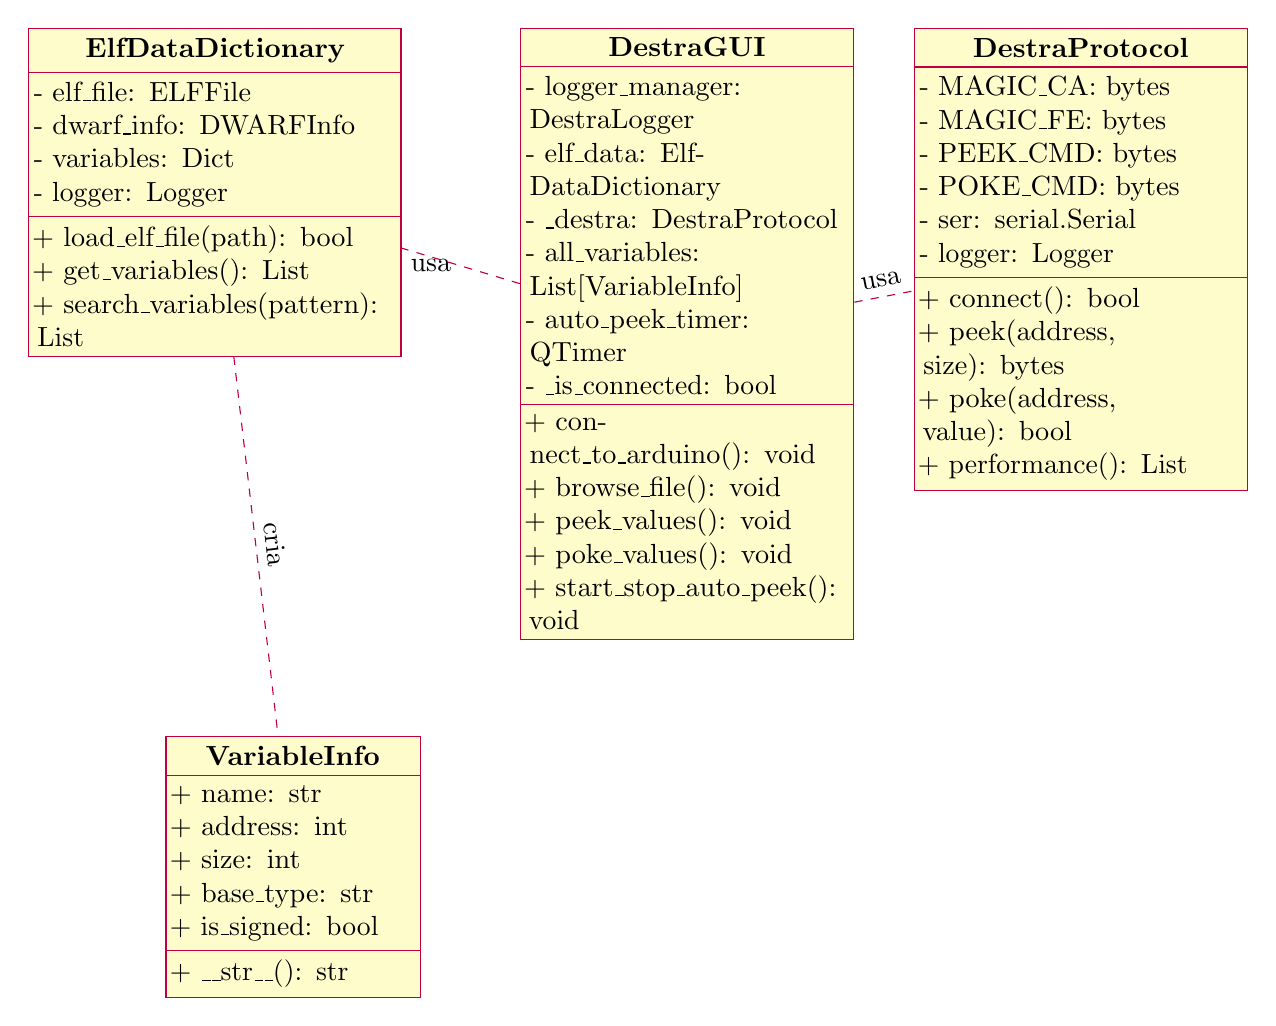
\begin{tikzpicture}[scale=1.0, transform shape]

% DestraGUI (Interface Principal)
\begin{class}[text width=4cm]{DestraGUI}{3,6}
\attribute{- logger\_manager: DestraLogger}
\attribute{- elf\_data: ElfDataDictionary}
\attribute{- \_destra: DestraProtocol}
\attribute{- all\_variables: List[VariableInfo]}
\attribute{- auto\_peek\_timer: QTimer}
\attribute{- \_is\_connected: bool}
\operation{+ connect\_to\_arduino(): void}
\operation{+ browse\_file(): void}
\operation{+ peek\_values(): void}
\operation{+ poke\_values(): void}
\operation{+ start\_stop\_auto\_peek(): void}
\end{class}

% DestraProtocol (Protocolo de Comunicação)
\begin{class}[text width=4cm]{DestraProtocol}{8,6}
\attribute{- MAGIC\_CA: bytes}
\attribute{- MAGIC\_FE: bytes}
\attribute{- PEEK\_CMD: bytes}
\attribute{- POKE\_CMD: bytes}
\attribute{- ser: serial.Serial}
\attribute{- logger: Logger}
\operation{+ connect(): bool}
\operation{+ peek(address, size): bytes}
\operation{+ poke(address, value): bool}
\operation{+ performance(): List}
\end{class}

% ElfDataDictionary (Análise de Arquivos ELF)
\begin{class}[text width=4.5cm]{ElfDataDictionary}{-3,6}
\attribute{- elf\_file: ELFFile}
\attribute{- dwarf\_info: DWARFInfo}
\attribute{- variables: Dict}
\attribute{- logger: Logger}
\operation{+ load\_elf\_file(path): bool}
\operation{+ get\_variables(): List}
\operation{+ search\_variables(pattern): List}
\end{class}

% VariableInfo (Informações de Variável)
\begin{class}[text width=3cm]{VariableInfo}{-2,-3}
\attribute{+ name: str}
\attribute{+ address: int}
\attribute{+ size: int}
\attribute{+ base\_type: str}
\attribute{+ is\_signed: bool}
\operation{+ \_\_str\_\_(): str}
\end{class}

% Relacionamentos
\draw[umlcd style dashed line] (DestraGUI) -- node[above, sloped, black]{usa} (DestraProtocol);
\draw[umlcd style dashed line] (DestraGUI) -- node[left, black]{usa} (ElfDataDictionary);
\draw[umlcd style dashed line] (ElfDataDictionary) -- node[above, sloped, black]{cria} (VariableInfo);

\end{tikzpicture}
\caption{Diagrama de Classes da Aplicação DESTRA UI}
\label{fig:diagrama_classes_destra}
\end{figure}

\section{Descrição das Classes}

\subsection{DestraGUI}
Classe principal da interface gráfica, herda de \texttt{QMainWindow}. Responsável por:
\begin{itemize}
    \item Gerenciar a interface do usuário com PySide6/Qt
    \item Coordenar as operações entre protocolo e análise ELF
    \item Implementar funcionalidades de auto-peek
    \item Gerenciar tabelas de variáveis disponíveis e selecionadas
\end{itemize}

\subsection{DestraProtocol}
Implementa o protocolo de comunicação serial com o Arduino:
\begin{itemize}
    \item Define comandos PEEK, POKE e PERFORMANCE
    \item Gerencia conexão serial e detecção automática de portas
    \item Processa respostas do protocolo com verificação de integridade
    \item Decodifica tipos de dados recebidos
\end{itemize}

\subsection{ElfDataDictionary}
Analisador de arquivos ELF com informações DWARF:
\begin{itemize}
    \item Extrai informações de variáveis (nome, endereço, tipo, tamanho)
    \item Processa estruturas, arrays e tipos básicos
    \item Fornece funcionalidades de busca e filtragem
    \item Gera estatísticas do arquivo analisado
\end{itemize}

\subsection{VariableInfo}
Estrutura de dados (dataclass) que armazena informações de uma variável:
\begin{itemize}
    \item Nome da variável
    \item Endereço de memória
    \item Tamanho em bytes
    \item Tipo base (uint8, uint16, uint32, etc.)
    \item Informações sobre sinalização e ponteiros
\end{itemize}

\subsection{DecodedTypes}
Classe utilitária para decodificação de tipos de dados:
\begin{itemize}
    \item Mapeia tipos de dados para formatos struct
    \item Fornece informações de tamanho por tipo
    \item Lista tipos suportados pelo sistema
\end{itemize}

\section{Padrões de Design Utilizados}

\subsection{Singleton}
A classe \texttt{DestraLogger} implementa o padrão Singleton para garantir uma instância única de configuração de logging em toda a aplicação.

\subsection{Model-View-Controller (MVC)}
A arquitetura segue parcialmente o padrão MVC:
\begin{itemize}
    \item \textbf{Model}: \texttt{ElfDataDictionary}, \texttt{VariableInfo}, \texttt{PerformanceData}
    \item \textbf{View}: \texttt{DestraGUI} e componentes Qt (QTableWidget, QComboBox, etc.)
    \item \textbf{Controller}: Métodos da \texttt{DestraGUI} que coordenam Model e View
\end{itemize}

\subsection{Data Transfer Object (DTO)}
As classes \texttt{VariableInfo} e \texttt{PerformanceData} funcionam como DTOs, transportando dados estruturados entre diferentes camadas da aplicação.

\subsection{Facade}
A classe \texttt{DestraProtocol} atua como uma facade, simplificando o acesso ao protocolo de comunicação serial complexo.

\end{document}
